\usetikzlibrary{shapes.geometric, arrows}
\lstset{literate={_}{\_}1} % This treats underscores as normal characters
\chapter{Resultados}
\label{cap:Resultados}

En este capítulo se detallarán todos los desarrollos realizados para la consecución de este TFM. El contenido se organizará en varias secciones, siguiendo las iteraciones identificadas en el capítulo ~\ref{cap:Metodologia}. En cada sección, se describirán las fases de Inicio, Elaboración, Construcción y Transición, de acuerdo con la metodología \ac{PUD}.

\section{Iteración 1 - Modelo del sistema}
\label{sec:it1-modelo-sistema}

En esta fase se describe la problemática planteada, las características que presentará la plataforma de cómputo escogida en este trabajo, y los requisitos mínimos que deberían ser cumplidos por cualquier otro sistema sobre el que se quieran realizar las mismas pruebas.

Tal y como se ha visto en los capítulos ~\ref{cap:Introduccion} y ~\ref{cap:Objetivo}, se pretende desarrollar un modelo teórico de energía válido para arquitecturas \ac{ARM}. Para poder realizar un modelo preciso, es necesario contar con unas métricas igual de precisas; por tanto, será necesario el uso de herramientas que den esa granularidad requerida, con el objetivo de obtener unas mediciones de consumo lo más exactas posible. En este contexto, el modelo planteado se ha decidido implementar en dos escenarios:

\begin{enumerate}[noitemsep]
    \item Mediante el despliegue de simulaciones con el programa Gem5
    \item Utilizando \ac{PAPI} en la plataforma física
\end{enumerate}

Sobre los dos escenarios, se dará finalmente una validación del modelo teórico en cuestión comparando los resultados con mediciones reales sobre el cable de corriente de la plataforma física, obtenidas con un \ac{DMM}.
En el contexto de este trabajo, se ha empleado la plataforma \ac{SBC} Raspberry Pi 4 Model B, basada en la arquitectura \ac{ARM}, con núcleos Cortex-A72, y frecuencia máxima 1.5GHz. Por defecto, este sistema no soporta \ac{DVFS}, aunque en recientes actualizaciones del \textit{firmware} es posible de configurar este parámetro en el fichero \textit{config.txt} \cite{dvfs-raspi}. Sin embargo, ésta opción no se ha tenido en cuenta en el contexto de este \ac{TFM}, de manera que se tendrá un voltaje constante y dos estados de frecuencia (baja frecuencia o \textit{idle} y alta frecuencia o \textit{activo}). Una imagen del dispositivo en cuestión se presenta en la figura ~\ref{fig:rpi4}.

\begin{figure}[ht!]
    \centering
    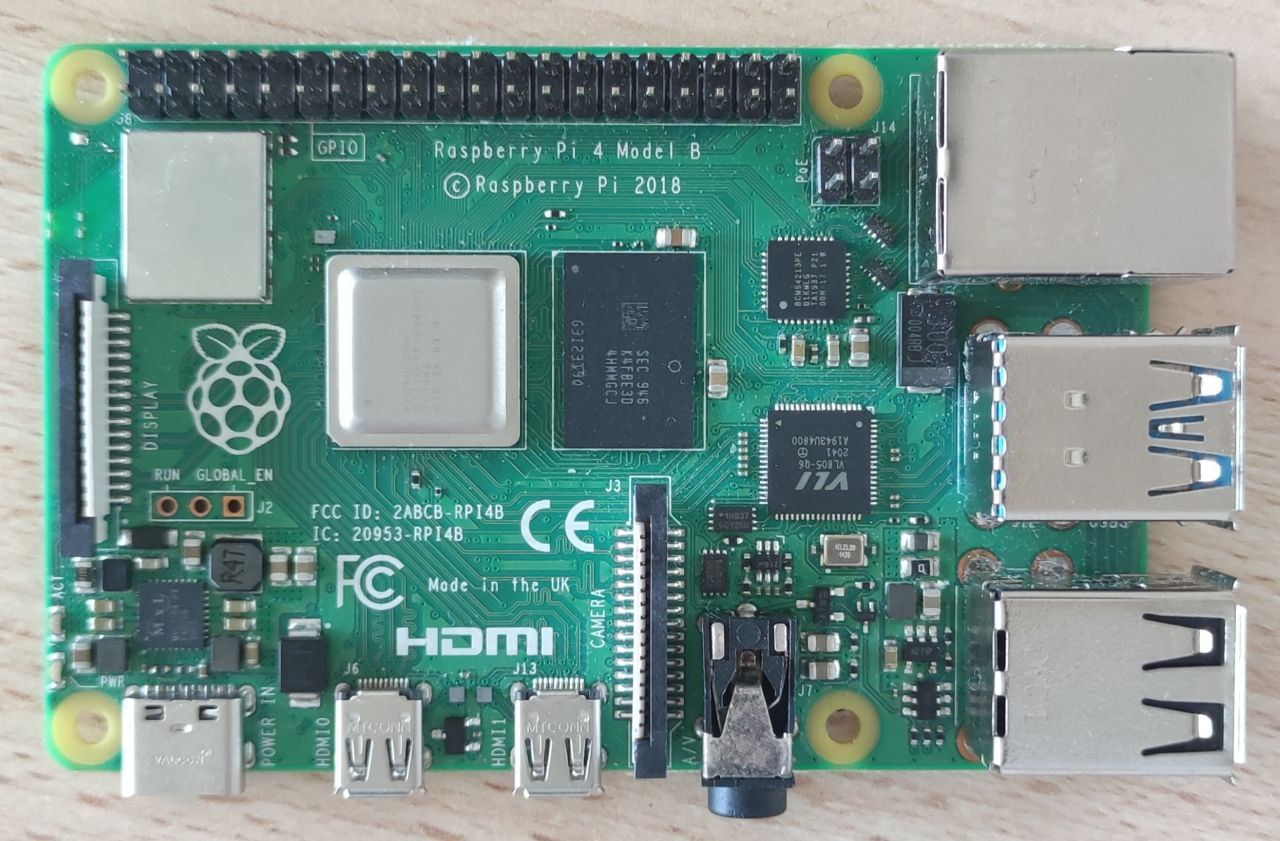
\includegraphics[width=0.6\linewidth, height=0.35\textwidth]{figs/rpi4.jpg}
    \caption{Raspberry Pi 4, Model B}
    \label{fig:rpi4}
\end{figure}

De acuerdo a la página oficial\footnote{Raspberry Pi 4: \url{https://www.raspberrypi.com/products/raspberry-pi-4-model-b/specifications/}} ~\cite{datasheetA72} se tienen las siguientes características clave:

\begin{itemize}[noitemsep]
    \item Procesador Broadcom BCM2711, Cuatro núcleos \ac{ARM} Cortex-A72, a 1.5GHz
    \item Memoria \ac{RAM} \ac{LPDDR4}, a 3200 MHz.
    \item Módem \ac{WiFi} IEEE 802.11ac, doble banda (2.4GHz y 5GHz).
    \item Módem Bluetooth 5.0, compatible con el estándar \ac{BLE}.
    \item Interfaz Gigabit Ethernet (10/100/1000 Mbps).
    \item Cuatro puertos \ac{USB} (siendo dos de ellos \ac{USB} 3.0, y los otros dos \ac{USB} 2.0).
    \item Dos puertos \ac{MicroHDMI} para salida de vídeo.
    \item 40 pines \ac{GPIO}.
    \item Alimentación con interfaz \ac{USB}-C.
    \item Caché L1 (instrucciones) de 48kB, \textit{three-way-associative}, organizada en líneas de 64B
    \item Caché L1 (datos) de 32kB, \textit{two-way-associative}, organizada en líneas de 64B
    \item Caché L2 (instrucciones y datos), de 1MB, \textit{16-way-associative}, organizada en líneas de 64B
\end{itemize}

En lo relativo a las unidades de cálculo \ac{ALU} y \ac{FPU}, el \ac{ARM} Cortex-A72 tiene dos canales de operaciones ALU simples y canales separados para operaciones complejas y \textit{branching} ~\cite{datasheetA72}. Cada canal de enteros tiene una cola de emisión de 8 entradas, mientras que el canal de ramas tiene una cola de 10 entradas. Por lo tanto, el núcleo puede tener hasta 34 micro-operaciones esperando una unidad de ejecución de enteros. Por otro lado, la FPU posee dos canales para manejar operaciones de punto flotante y vectoriales, cada uno alimentado desde una cola de emisión de tamaño modesto con 8 entradas. El rendimiento vectorial es modesto, ya que la mayoría de las instrucciones de 128 bits se ejecutan a media velocidad. A modo de comparación, para la Raspberry Pi 3, el modelo anterior, estas características son más modestas ~\cite{datasheetA53} pero similares, con doble canal tanto ALU como para FPU.

Posteriormente, se ha verificado el correcto funcionamiento del sistema, probándose a nivel funcional. Además, se ha configurado para poder operar sobre la misma sin necesidad de utilizar periféricos o depender de conexiones \ac{SSH}. Esto se ha logrado activando el puerto \ac{UART} de la Raspberry Pi, algo fácil de realizar gracias a la herramienta \textit{raspi-config}, disponible de forma nativa en Raspberry Pi OS. Al activar esta interfaz \ac{UART} y deshabilitar \textit{Bluetooth} (este último acapara el primer conjunto \ac{UART} por defecto) es posible este planteamiento. De esta forma, se consigue un menor ruido en las mediciones de consumo y de cómputo a la hora de realizar cualquier tipo de ejecución sobre la plataforma física. En la figura~\ref{fig:activarUART} se muestra el proceso de activación de \ac{UART}.

\begin{figure}[H]
    \centering
    \begin{subfigure}[b]{0.49\textwidth}
        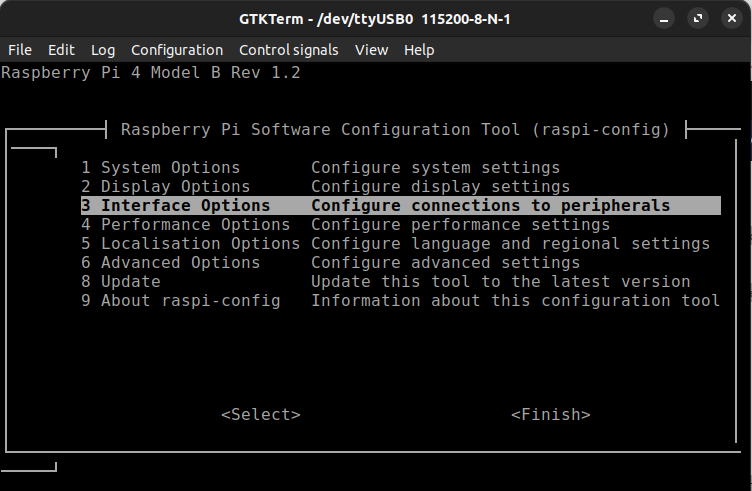
\includegraphics[width=\textwidth]{figs/raspiconfig-opcion3.png}
        \caption{Entrando en raspi-config y selección de opción 3}
        \label{fig:activarUART1}
    \end{subfigure}
    \hfill
    \begin{subfigure}[b]{0.49\textwidth}
        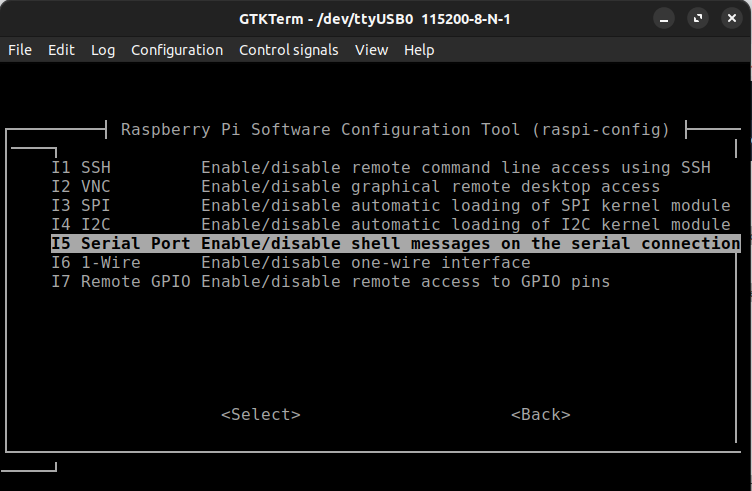
\includegraphics[width=\textwidth]{figs/raspiconfig-activarUART.png}
        \caption{Activación de puerto serie (\ac{UART})}
        \label{fig:activarUART2}
    \end{subfigure}
    \caption{Proceso de activación del \ac{UART}}
    \label{fig:activarUART}
\end{figure}

Para finalizar, se ha decidido realizar un \textit{script} que deshabilite servicios innecesarios. El listado ~\ref{lst:desactivarServicios} muestra el proceso que controla que el usuario ejecutando el \textit{script} sea root, para luego ir deshabilitando los servicios uno por uno. Estos servicios se seleccionaron mediante el comando de terminal $systemd-analize blame$, el cual muestra el tiempo de ejecución invertido en cada uno de los servicios del sistema, ordenados por mayor a menor tiempo. Los servicios desactivados son aquellos que tienen el mayor tiempo de ejecución y que, a la vez, no son críticos para el sistema operativo, como el conjunto de servicios pertenecientes a \textit{NetworkManager} \cite{networkmanager} o las interfaces de red \ac{WiFi}. En el listado \ref{lst:desactivarServicios}, en la sección de Anexos, por motivos de espacio, se muestra un \textit{script} realizado para desactivar servicios e interfaces de automáticamente

En el contexto de este \ac{TFM}, es prioritario cumplir con una serie de características por parte del modelo de sistema a caracterizar energéticamente. En ~\ref{tab:requisitos} se presentan los requisitos más importantes que la plataforma debe cumplir.

\begin{itemize}[noitemsep]
    \item \label{tab:requisitos}\textbf{Soporte para lectura de eventos \textit{hardware}}: la plataforma utilizada debe tener registros contadores de ciertos eventos \textit{hardware} y ser capaz de acceder a ellos.

    \item \textbf{Basado en arquitectura \ac{ARM} moderna}: como requisito mínimo, el modelo debe basarse en un \ac{ISA} \textit{ARMv8-A}, del 2011, siendo la primera con capacidad para ejecutar aplicaciones en modo 64bit y tener los eventos \textit{hardware} implementados en forma de registros \cite{arm-a}

    \item \textbf{Acceso efectivo a usuario \textit{root}}: es necesario tener permisos de superusuario para poder configurar el acceso de lectura de los eventos \textit{hardware}.
\end{itemize}

Además las características presentadas, es necesario que la plataforma escogida debe poder acceder, como mínimo, a los registros mostrados en ~\ref{lst:eventoshw}, los cuales, en el Cortex-A72, son manejados por la unidad \ac{PMU}. Los nombres se corresponden con los de la plataforma utilizada en este trabajo, obtenidos del \ac{ARM} Cortex-A72 MPCore Processor Technical Reference Manual ~\cite{referencia-a72}, por lo que la nomenclatura puede diferir en caso de usar otra arquitectura.

\begin{table}[H]
\footnotesize
\centering
    \begin{tabular}{|
    >{\columncolor[HTML]{C0C0C0}}c |c|}
    \hline
    \cellcolor[HTML]{9B9B9B}\textbf{DESCRIPCIÓN}                                                      & \cellcolor[HTML]{9B9B9B}\textbf{EVENTO (CORTEX-A72)} \\ \hline
    \cellcolor[HTML]{C0C0C0}\textbf{Número de ciclos}                                                 & CPU\_CYCLES                                                    \\ \hline
    \cellcolor[HTML]{C0C0C0}                                                                          & L1D\_CACHE\_ACCESS                                             \\ \cline{2-2} 
    \multirow{-2}{*}{\cellcolor[HTML]{C0C0C0}\textbf{Accesos totales en caché L1}}                    & L1I\_CACHE\_ACCESSES                                           \\ \hline
    \textbf{Número instrucciones ejecutadas}                                                          & INST\_SPEC\_EXEC                                               \\ \hline
    \cellcolor[HTML]{C0C0C0}                                                                          & INST\_SPEC\_EXEC\_INTEGER\_INST                                \\ \cline{2-2} 
    \multirow{-2}{*}{\cellcolor[HTML]{C0C0C0}\textbf{Nº instrucciones aritmético-lógicas ejecutadas}} & INST\_SPEC\_EXEC\_VFP                                          \\ \hline
    \textbf{Fallos de escritura totales en caché de datos L1}                                         & L1D\_CACHE\_REFILL                                             \\ \hline
    \textbf{Accesos de lectura totales en caché de datos L1}                                          & L1D\_CACHE\_ACCESS                                             \\ \hline
    \textbf{Accesos totales en caché L2}                                                              & L2D\_CACHE\_ACCESS                                             \\ \hline
    \end{tabular}
\caption{Descripciones y eventos \textit{hardware} necesarios (Cortex-A72)}
\label{lst:eventoshw}
\end{table}

\vspace*{-0.2cm}

Finalmente, se presenta en \ref{fig:arquitecturaA72} se presenta el diagrama de bloques del Cortex-A72 en la plataforma Raspberry Pi 4. Como puede observarse, cada núcleo posee una \ac{PMU} que maneja eventos \textit{hardware}. Además, cada \textit{core} tiene una unidad de predicción de salto, unidades funcionales de cálculo de enteros y punto flotante, así como una unidad para la pila de llamadas realizadas. También, en otro bloque separado, se tienen los eventos misceláneos, donde se engloban interrupciones ($GIC$) y los temporizadores generales para cada núcleo. Por último, se tiene una caché de primer nivel por núcleo, accediéndose a datos e instrucciones mediante un \textit{arbitrer}; por otro lado, la caché de nivel 2 está compartida entre todos, estando el \textit{arbitrer} y los datos alojados en un bloque distinto.

\begin{figure}[H]
    \centering
    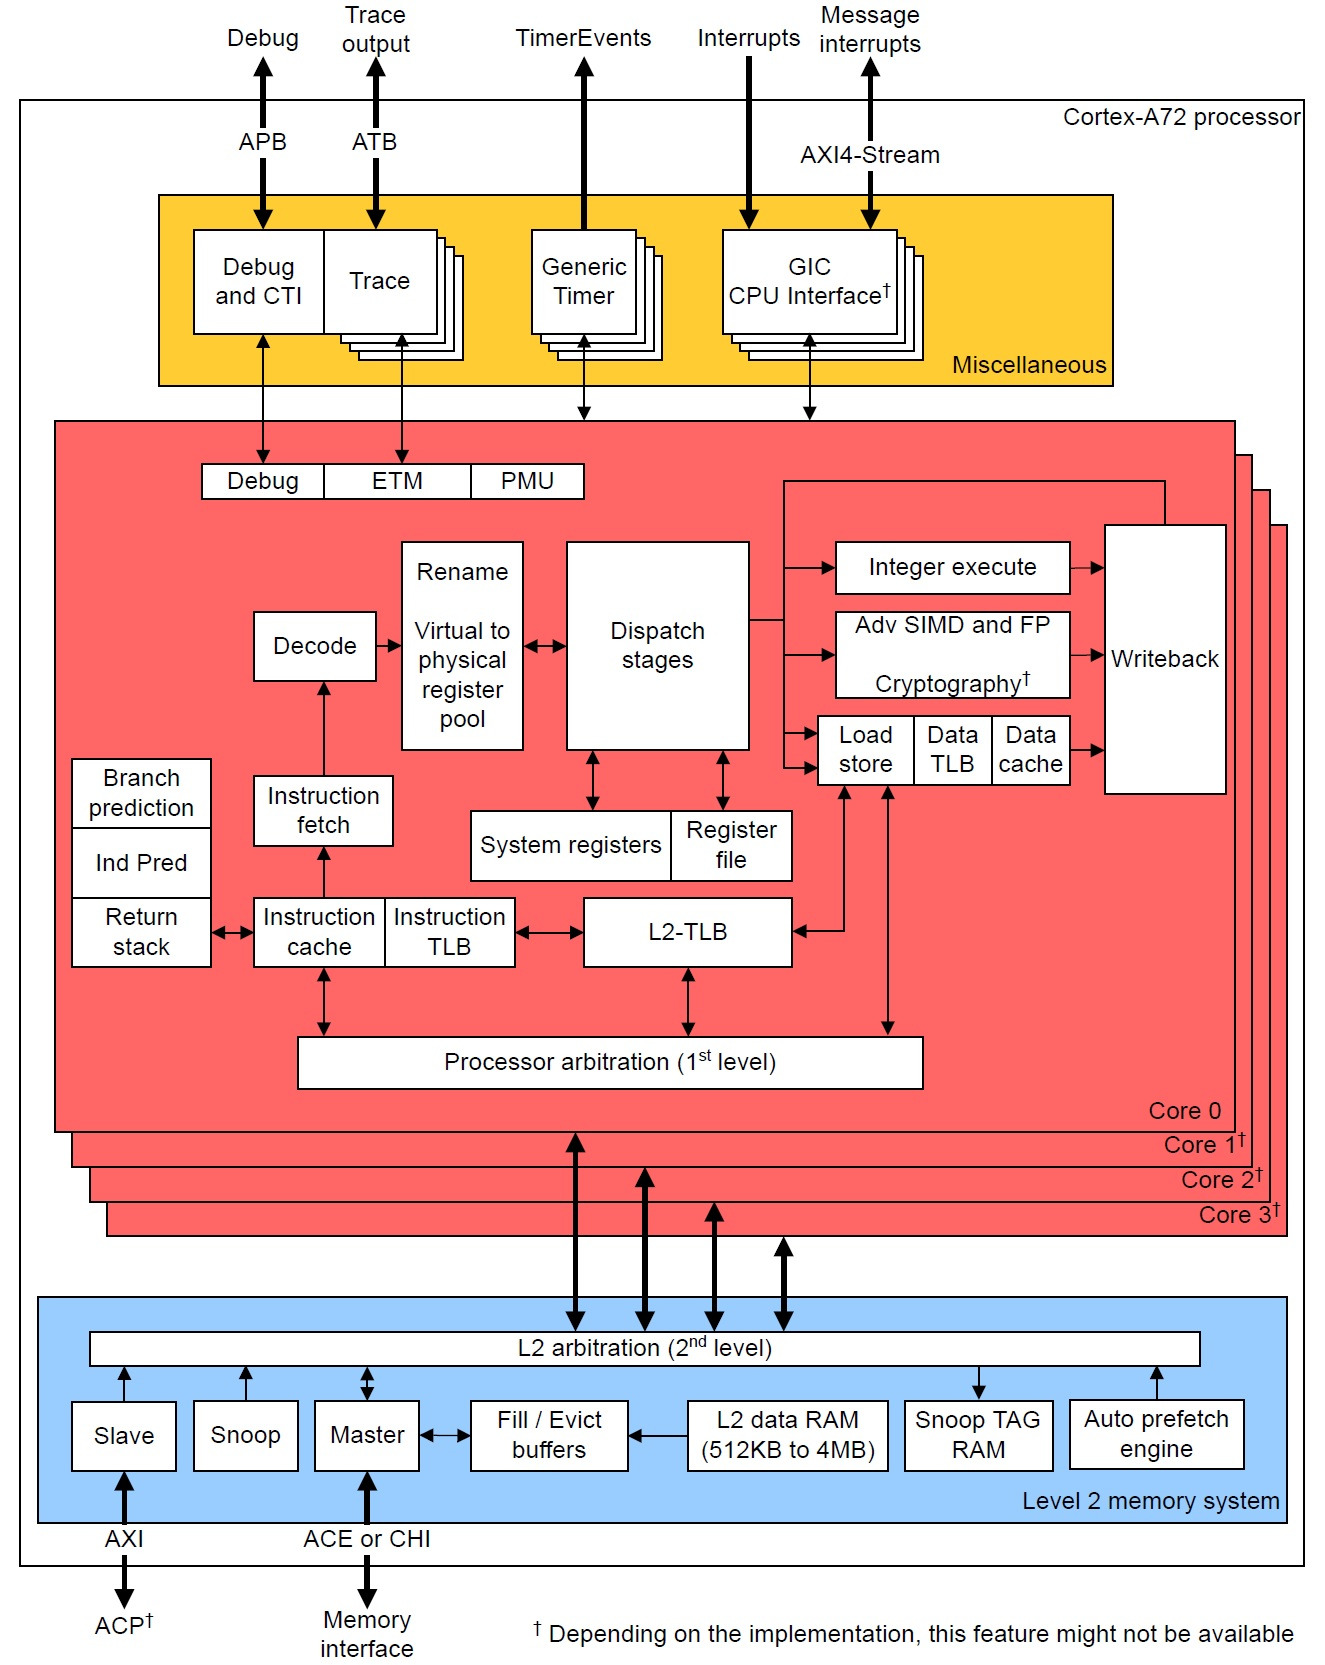
\includegraphics[width=0.75\linewidth, height=0.85\textwidth]{figs/Cortex-A72-BlockDiagram.jpg}
    \caption{Digrama de bloques del Cortex-A72 para la Raspberry Pi 4 \cite{datasheetA72}}
    \label{fig:arquitecturaA72}
\end{figure}

\pagebreak

\section{Iteración 2 - Elección del simulador}
\label{it2:eleccionSimulador}

Debido a lo expuesto en la sección~\ref{sec:Gem5-qemu-estado-arte}, el área de las simulaciones \textit{hardware} es un área cada vez más importante a la hora de caracterizar energéticamente una plataforma de cómputo, siendo especialmente interesante si no se tiene una referencia previa del coste energético de la misma, o si no se tiene la plataforma en cuestión. En este contexto, realizar simulaciones de la plataforma puede ser de gran ayuda, dando una noción de partida en términos de consumo. Por ello, se emplearán en el desarrollo de este \ac{TFM}.

Además, se ha realizado una comparación detallada entre las dos principales opciones tenidas en cuenta dentro de ese trabajo: Gem5 y qEMU \ref{subs:qemu}. Aunque existen alternativas, como \ac{ARM} FastModels \cite{arm-fastmodels}; sin embargo, esta última herramienta es de pago (tras un mes de prueba) y de código propietario, además de solo permitir simular el componente procesador y realizar ciertas técnicas de \textit{profiling}, por lo que en cierta medida es más una simulación funcional de la arquitectura de un procesador concreto, siendo el objetivo de este trabajo distinto al de este simulador.

Tras comparar ambas opciones con las características presentadas en la tabla~\ref{tab:fortalezas_debilidades} se ha decidido seleccionar, en el contexto de este trabajo, al simulador Gem5 por encima de qEMU debido, entre otras, a las siguientes razones:

\begin{itemize}
    \item \textbf{Código fuente abierto}: el simulador Gem5 tiene alojado su código fuente al completo en un repositorio GitHub \cite{Gem5-github}, siendo completamente \textit{open-source} y no requerir de licencias.
    
    \item \textbf{Detallismo de las métricas obtenidas}: Gem5 permite obtener métricas muy precisas y variadas, aspecto muy útil en el desarrollo de un modelo de consumo energético sin referencias previas, donde se puede realizar mediante iteraciones y pesos una aproximación a la realidad.
    
    \item \textbf{Simulaciones a nivel de ciclo}: esta característica está relacionada con la anterior; el poder simular a nivel de ciclo permite ver de forma mucho más precisa que otras alternativas el número de instrucciones relativas a una tarea o \textit{benchmark} concretos.
    
    \item \textbf{Personalización de la plataforma a simular}: Gem5 permite personalizar cada uno de los componentes del sistema. Así, se puede simular una arquitectura \textit{hardware} lo más parecida a la plataforma física.
\end{itemize}

\section{Iteración 3 - Desarrollo del marco teórico}

\paragraph{}{
\label{estadoArteModelos}
En esta iteración se mostrará el procedimiento llevado a cabo para realizar el marco teórico de medición. Se comenzará exponiendo los modelos de consumo estudiados, para finalmente presentar la metodología desarrollada para aplicar el marco de medición.

Tras el estudio del estado del arte de los conceptos clave que es necesario comprender para desarrollar un modelo de estimación del consumo para una plataforma de cómputo, tal y cómo se explicó en~\ref{subs:conceptos-electricidad}, se han identificado dos planteamientos posibles dentro de este \ac{TFM} para el desarrollo del modelo teórico:

\begin{enumerate}
    \item La energía como el sumatorio de energías de componentes \textit{hardware} individuales y relevantes dentro del \ac{IC} durante el tiempo de ejecución de la aplicación.
    
    \item La energía como la suma de potencia dinámica y estática del procesador durante el tiempo de ejecución de la aplicación .
\end{enumerate}


En primer planteamiento, se identifican las operaciones que suponen mayor peso al ejecutar una aplicación determinada, así como las tareas principales identificadas. Cada tarea se caracteriza por utilizar un determinado componente hardware que requiere una cierta energía para su ejecución durante un tiempo determinado. Por tanto, formalmente una tarea se define como una tupla intensidad-tiempo, en amperios y en segundos, respectivamente, donde $V$ corresponde al voltaje utilizado por la plataforma, cada elemento i-ésimo corresponde con un componente hardware, su intensidad $I_i$ y su tiempo de ejecución $t_i$. De esta forma, se obtiene la fórmula que se muestra en \ref{eq:energiaModelo1}:

\begin{equation}
    E_\mathcal{A}=\sum_{i=1}^n I_i \times t_i \times V \forall t_i  \in \mathcal{A}
    \label{eq:energiaModelo1}
\end{equation}

Por otro lado, para el segundo planteamiento, realizado en \cite{soton393728} \cite{soton418538}, el enfoque es distinto: en este caso, se identifican, dentro del componente procesador, los valores de rendimiento más importantes en términos de consumo mediante eventos \textit{hardware}. Para cada unidad dentro del procesador identificada como relevante para el modelo teórico se realiza un cálculo de potencia dinámica. El sumatorio de cada una de ellas, a la vez que se añade la potencia estática generada por el \textit{chip}, da lugar a la potencia global, mostrada en \ref{eq:potenciaDinamicaEstatica}.

\begin{equation}P = P_{dyn} + P_{st}\label{eq:potenciaDinamicaEstatica}\end{equation}

Por último, para calcular la energía, y sabiendo las fórmulas de la potencia dinámica y estática, se multiplica el valor global de ésta por el tiempo total de ejecución $t$, obteniéndose la fórmula en \ref{eq:energiaModelo2}

\begin{equation}E = P \times t\label{eq:energiaModelo2}\end{equation}
}

\paragraph{}{
\label{subs:comparativaModelos}
En el contexto de ese trabajo, se han tenido en cuenta los dos planteamientos expuestos en \ref{estadoArteModelos}, mientras que, a continuación, se exponen las principales ventajas e inconvenientes. }

\begin{itemize}
    \item Con el primer planteamiento, se tiene una mayor simplicidad y escalabilidad, ya que es posible de extender su uso a periféricos externos, como un módulo de comunicaciones \ac{WiFi} conectado por \ac{USB}. Además, es relativamente sencillo de establecer las referencias base, bastando la lectura de las \textit{datasheets} para averiguar los valores de corriente y voltaje máximos. Como gran inconveniente, se tiene la poca precisión obtenida del mismo, precisamente por no poseer un factor de actividad y categorizar todo el tiempo de ejecución como estado activo, cuando, en la realidad, no es así \cite{antoniomateo}.

    \item Con el segundo planteamiento, se obtiene una mayor precisión en los resultados obtenidos, gracias en parte a entrar el concepto de potencia dinámica \cite{soton393728} \cite{soton418538}, lo que permite tener en cuenta un factor de actividad que determine el tiempo de actividad relativo del procesador, así como la capacitancia del mismo. Además, gracias a los cálculos realizados de las fugas teóricas de corriente, es posible también realizar una estimación de la potencia estática. Como principales inconvenientes se encuentran el que los valores de capacitancia y factor de actividad se han tomado directamente de \cite{soton393728} y \cite{soton418538}, aunque, como línea base del modelo a desarrollar, se ha considerado positivo utilizar los resultados de éstos. Por último, otro gran inconveniente es que este modelo solo tiene en cuenta al procesador, y no a la plataforma al completo; si bien es posible ampliar el modelo, calculando los valores necesarios para cada componente a añadir, no está contemplado dentro del contexto de este \ac{TFM}, debido principalmente a que los programas para validar el modelo son especialmente intensivos en \ac{CPU}. \\
\end{itemize}

Finalmente, se ha decido seleccionar el segundo modelo planteado por:

\begin{itemize}
    \item \textbf{Orientado a \ac{CPU}}: debido a que los programas para validar el modelo son intensivos en \ac{CPU}, es especialmente interesante el segundo modelo, centrado en este componente, debido a la naturaleza de los programas de pruebas empleados para la validación del modelo

    \item \textbf{Mayor precisión en los resultados}: el segundo modelo es capaz de obtener valores más precisos de consumo gracias a la inclusión de la potencia dinámica y estática, así como de valores de referencia para la capacitancia y el factor de actividad de una plataforma de cómputo. \\
\end{itemize}

Tras proporcionar las definiciones clave, así como el estado del arte en modelos teóricos de consumo para plataformas de cómputo, seleccionando uno de ellos posteriormente, se explicará, en esta fase, los pasos realizados para diseñar el marco de medición teórico del consumo energético. Nuevamente, solamente se ha incluido el componente procesador como el único para caracterizar, pero esta metodología es extrapolable a diferentes componentes dentro de la plataforma, tales como memoria \ac{RAM}, o memoria secundaria, siendo en el contexto de este trabajo, el lector de \ac{microSD}. El marco de medición presentado se ha desarrollado siguiendo una metodología diseñada concretamente para este \ac{TFM}. Los puntos clave de la misma son:

\begin{enumerate}[noitemsep]
    \item Obtención de valores de capacitancia y factor de actividad del componente (\ac{CPU}, \ac{RAM}, etc.).
    \item Obtención del valor de las fugas de corriente.
    \item Lectura de toda la documentación disponible.
    \item Desarrollo de un entorno apto para realizar simulaciones \textit{hardware} y obtener estadísticas.
    \item Selección de \textit{benchmarks} relevantes en consumo energético.
    \item Desarrollo de un entorno apto para realizar ejecuciones sobre la plataforma física, y lectura los eventos de \textit{hardware} correspondientes.
    \item Construcción de tablas que contengan las métricas más relevantes para cada componente, así como los casos de uso más importantes, y rellenado de las mismas con la energía consumida por el componente ante diferentes escenarios de ejecución.
\end{enumerate}

Por tanto, el objetivo de la metodología propuesta es la definición de un marco de validación de una plataforma de cómputo a nivel energético, mediante una serie de pasos que puedan ser reutilizados para medir diferentes componentes del sistema. En el contexto de este \ac{TFM}, se ha trabajado únicamente sobre el componente procesador, considerándose como la primera aproximación para la construcción del modelo de energía.
Finalmente, se muestra en la figura ~\ref{fig:pasos_metodologia} un diagrama de flujo con los pasos que conforman la metodología desarrollada. En ésta, primero se escriben los programas \textit{benchmark} y se seleccionan los escenarios más importantes en cada caso. Posteriormente, se obtienen las métricas de electricidad necesarias para el modelo de consumo, como la capacitancia, factor de actividad, potencia, etcétera, para el componente a caracterizar. Después se realizan, de forma paralela, el lanzamiento de simulaciones con Gem5, y el lanzamiento de las mismas pruebas sobre la plataforma real, con PAPI. Ambas actividades generan una serie de estadísticas, las cuales son comparadas para ver el comportamiento general en cada escenario. Con los datos obtenidos por ambas vías se construirán una serie de tablas comparativas y gráficos, para posteriormente calcular el consumo de energía estimado tras aplicar el modelo teórico. Finalmente, ambos escenarios serán validados mediante la comparación de resultados frente a mediciones reales obtenidas con un DMM. En caso positivo, se da el modelo por validado. En caso negativo, se vuelve a comenzar el proceso de validación refinando los valores de electricidad previos. 

\pagebreak

\begin{figure}[H]
    \centering
    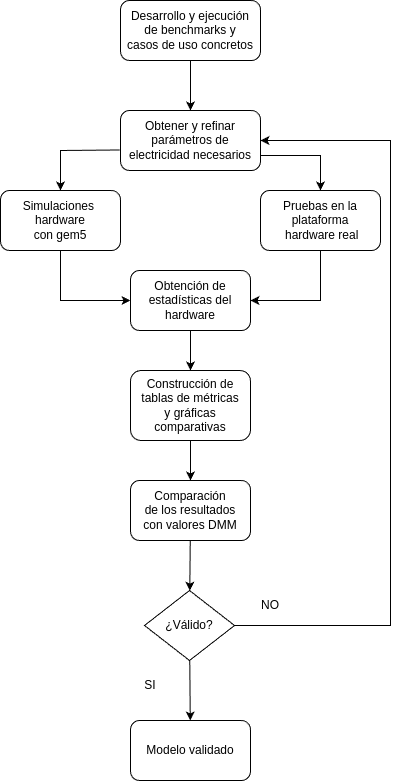
\includegraphics[width=0.65\linewidth, height=1.15\textwidth]{figs/Metodologia_TFM.png}
    \caption{Metodología desarrollada para este trabajo}
    \label{fig:pasos_metodologia}
\end{figure}

\section{Iteración 4 - Configuración del entorno para Gem5}

En esta iteración se ha realizado el diseño de programas destinados a su ejecución en la plataforma \textit{hardware} simulada, basada en la plataforma física utilizada, la Raspberry Pi 4, con el simulador Gem5. Para comenzar, se desarrollarán los principales conceptos clave para esta iteración. Posteriormente se expondrán las configuraciones realizadas para poder utilizar el simulador en este trabajo.
Finalmente, se presentará el código de los \textit{benchmarks} utilizados dentro de este \ac{TFM}, así como los ficheros más relevantes a la hora de ejecutar simulaciones y \textit{scripts} de automatización de las tareas en esta iteración.

\subsection{Conceptos fundamentales}
\subsubsection{\textit{Kernel}}
\label{subs:kernel}
El \textit{kernel}, a menudo denominado núcleo, es el \textit{alma mater} del sistema operativo. Actúa como un puente entre el \textit{hardware} y el software, gestionando los recursos del sistema, controlando la ejecución de programas y brindando una plataforma estable para que operen las aplicaciones. En esta situación, será el \textit{kernel} el que se encargue de tareas críticas como la gestión de memoria, la programación de procesos, la entrada/salida y la seguridad. A lo largo de los años, el kernel de Linux ha evolucionado para ofrecer un alto rendimiento, estabilidad y confiabilidad.

\subsubsection{\textit{Bootloader}}
\label{subs:bootloader}
El \textit{bootloader} (cargador de arranque) es el responsable de iniciar el sistema operativo cuando se enciende el computador. Sirve como intermediario entre el \textit{firmware} del \textit{hardware} y el kernel, cargando este último en la principal (RAM) y preparando el entorno para que el sistema operativo pueda funcionar correctamente. Este componente también puede ofrecer opciones de configuración y herramientas de diagnóstico antes de iniciar el sistema operativo. Esta característica se puede encontrar, por ejemplo, en los cargadores de arranque del \ac{SO} Android.

\subsubsection{DTB}
\label{subs:dtb}
El \ac{DTB} es un fichero de descripción de cada uno de los componentes del sistema. Este fichero está compilado para una arquitectura del procesador concreta con el objetivo de que el sistema operativo sea capaz de mapear en memoria cada componente existente en el sistema y así manejar de forma eficiente cada elemento. Todo fichero \ac{DTB} tiene su base en un fichero fuente, el \ac{DTS}, interpretable para el ser humano, donde se especifica cada componente. Para la obtención del \ac{DTB} es necesario compilar el \ac{DTS} con la herramienta \textit{dtc}, integrada en el \textit{kernel} de Linux. 

\subsubsection{GIC}
\label{subs:gic}
El \ac{GIC} es un componente fundamental en los sistemas basados en \ac{ARM}, encargado de gestionar las interrupciones de los periféricos. Actúa como un intermediario entre los dispositivos externos y el procesador, permitiendo que este último responda a los diferentes eventos que suceden en tiempo de ejecución, como la llegada de datos, errores o cambios de estado. El GIC se encarga de priorizar interrupciones, enrutarlas hacia los núcleos de procesamiento adecuados y proporcionar mecanismos para enmascararlas, si es necesario, según las necesidades del sistema. 

\subsubsection{Memoria principal}
\label{subs:ram}
La memoria principal, también conocida como memoria RAM (Random Access Memory), es un componente esencial en la informática, proporcionando almacenamiento temporal y acceso rápido a datos e instrucciones que el procesador necesita ejecutar en cada momento. La memoria RAM es volátil, esto es, que pierde su contenido al completo, cuando el sistema se apaga. En la actualidad, la memoria principal ha evolucionado significativamente para abordar las crecientes demandas de rendimiento en aplicaciones modernas. Las \ac{DRAM}, como \ac{DDR} en sus múltiples estandarizaciones por parte del organismo \ac{JEDEC}, como \ac{DDR4}, son tipo de memoria principal más extendido en la actualidad. En el contexto de este trabajo, es relevante las versiones de menor voltaje, y por tanto, menor consumo, como el estándar \ac{LPDDR4}, utilizado en la plataforma de pruebas escogida, la Raspberry Pi 4.

\subsubsection{Memoria secundaria}
\label{subs:discoduro}
La memoria no volátil, como el disco duro o la unidad de estado sólido, es el repositorio de almacenamiento permanente del sistema. Almacena datos y programas incluso cuando el sistema está apagada, lo que garantiza la persistencia de la información y la capacidad de reiniciar el sistema desde un estado conocido. La memoria no volátil es crucial para el funcionamiento a largo plazo del sistema operativo y la conservación de datos esenciales. Este apartado es especialmente relevante en el simulador Gem5, donde para poder ejecutar una simulación es crucial tener una imagen de disco que contenga lo necesario para que \textit{kernel} y \textit{bootloader} puedan funcionar. 

\subsubsection{Bus}
\label{subs:bus}
El bus es la forma que tiene una plataforma de cómputo para mover información (datos e instrucciones) entre los diferentes componentes del sistema (memorias, procesador, etcétera). Los buses pueden ser de memoria o de datos, siendo precisamente esa la diferencia entre las arquitecturas de computadores Von Neumann (más antigua) y Harvard (actual), siendo para el primero un único tipo de bus para todo, y en el segundo dos tipos distintos. A la hora de realizar simulaciones, es necesario configurar buses para poder comunicar los diferentes componentes de la plataforma. 

\subsubsection{Compilación cruzada}

  En el mundo de la informática, la compilación juega un papel fundamental en la transformación del código fuente escrito en un lenguaje de relativo alto nivel (C, C++, Java, etcétera) en programas ejecutables que pueden ser comprendidos y ejecutados por la máquina. En la realidad, la compilación no es un único proceso, sino que se desarrolla en varias etapas:

  \begin{itemize}
    \item \textbf{Análisis}: El código fuente se analiza para verificar su sintaxis y estructura, detectando posibles errores o inconsistencias gramaticales del lenguaje de programación utilizado.
    \item \textbf{Preprocesamiento}: Se realizan expansiones de macros, inclusiones de archivos y otras tareas de preprocesamiento según las directivas presentes en el código fuente.
    \item \textbf{Compilación}: El código fuente se traduce de un lenguaje de alto nivel, como C o Java, a un lenguaje de bajo nivel, como el lenguaje ensamblador específico del procesador del ordenador.
    \item \textbf{Ensamblado}: El código ensamblador se traduce en código máquina, que es el conjunto de instrucciones binarias que el procesador puede comprender y ejecutar directamente.
    \item \textbf{Enlazado}: Se combinan los archivos objeto generados en la etapa de ensamblado, junto con las bibliotecas necesarias, para crear un único ejecutable final.
  \end{itemize}

  Sin embargo, cuando se trata de entornos de desarrollo complejos, como los sistemas embebidos o el desarrollo para múltiples plataformas, surge la necesidad de la compilación cruzada, un proceso especial de compilación que permite generar código ejecutable para una plataforma de destino diferente a la del sistema donde se está realizando la compilación, principalmente por las pocas capacidades de cómputo que suelen presentar los dispositivos embebidos, o por simplificar el proceso de desarrollo de \textit{software} multiplataforma. Con la compilación cruzada, se posible generar un binario que pueda ejecutarse en una arquitectura distinta a la utilizada por la máquina empleada para el desarrollo del código: por ejemplo, un ordenador con x86, mediante esta técnica, es capaz de generar un ejecutable para, por ejemplo, aarch64 (\ac{ARM} 64 bits). En el contexto de este trabajo, este tipo de compilación ayuda enormemente al desarrollo de binarios para ejecutar en la plataforma a simular en el simulador Gem5. Asimismo, la herramienta utilizada para realizar este propósito ha sido el \textit{toolchain} de \ac{GCC} para aarch64, versión 11, disponible para x86 desde los repositorios oficiales en Ubuntu 22.04. 

\subsubsection{Utilidades m5 y m5ops}
\label{sec:configM5ops}

Las utilidades m5 y m5ops ~\cite{m5ops-documentacion} están integradas dentro del simulador \textit{hardware} Gem5, siendo las herramientas enfocadas en el lanzamiento de comandos o instrucciones especiales para realizar funciones determinadas, a priori, imposibles de realizar de forma automática. En el contexto de este \ac{TFM} destacan:

\begin{itemize}
    \item \textbf{checkpoint <\textit{delay}> <\textit{period}>}: crea un "punto de guardado", pasado un tiempo determinado, en nanosegundos (el \textit{delay}), repitiéndose la llamada cada X nanosegundos (el \textit{period}). Esta llamada es clave para poder restaurar simulaciones desde un punto concreto, ahorrándose tiempo en el lanzamiento de la simulación. Para la generación de un \textit{checkpoint} que permita reanudar rápidamente una simulación, se ha utilizado en un \textit{script} Bash que ejecuta el comando \textit{m5 checkpoint 500000}, donde 500000 es el \textit{delay} antes de hacer el punto de retorno. Es necesario un \textit{delay} para que el \textit{checkpoint} sea útil, ya que es necesario que el sistema se haya cargado completamente. El \textit{delay} asegura esto.
    
    \item \textbf{dumpstats <\textit{delay}> <\textit{period}>}: genera un nuevo conjunto de estadísticas, pasado un tiempo determinado, en nanosegundos (el \textit{delay}), repitiéndose la llamada cada X nanosegundos (el \textit{period}). Con esta llamada, es posible obtener, por tanto, los datos medidos para cada ejecución de los \textit{benchmarks}. Al emplearse funciones propias de las librerías de m5 dentro del código fuente, así, se reduce el \textit{overhead} en términos generales, así como en espacio de pila utilizado.
    
    \item \textbf{resetstats <\textit{delay}> <\textit{period}>}: hace un \textit{reseteo} de estadísticas, pasado un tiempo determinado, en nanosegundos (el \textit{delay}), repitiéndose la llamada cada X nanosegundos (el \textit{period}). De esta forma, se puede validar que los datos medidos para cada ejecución son, efectivamente, individuales a cada una de ellas. Nuevamente, al emplear funciones propias de las librerías de m5 dentro del código fuente, se reduce el \textit{overhead} general.

    \item \textbf{exit <\textit{delay}>}: termina la ejecución de la simulación, pasado un tiempo determinado, en nanosegundos (el \textit{delay}). No requiere un valor concreto, ya que las simulaciones están pensadas para finalizar en el menor tiempo posible.
    
\end{itemize}

El uso de estas llamadas, en el contexto de este trabajo, se ha realizado solo con el parámetro \textit{delay}, para evitar entrar en bucles inesperados dentro de las simulaciones por la inclusión de un período. Posteriormente se muestra en ~\ref{subs:usoGem5} cómo se han aplicado estas llamadas en los programas desarrollados. Además, como se verá posteriormente, las directivas utilizadas en cuestión tienen una nomenclatura sensiblemente distinta a la presentada, pero representando lo mismo.

\subsubsection{El procesador en Gem5}
\label{subs:Gem5-procesador}

Según el punto de vista, los procesadores pueden clasificarse de una forma u otra. En el contexto de este trabajo, el procesador se valora principalmente en el modo de ejecución de las instrucciones. En este punto de vista, Gem5 clasifica a los procesadores en:

\begin{itemize}
    \item \textbf{In-Order}: siguen un enfoque secuencial y rígido para ejecutar instrucciones. Las instrucciones en un procesador \textit{in-order} se procesan una tras otra, sin saltarse ninguna. Si una instrucción necesita un resultado de la instrucción anterior, debe esperar a que esta se complete. Aunque este método es más sencillo de implementar y consume menos energía, puede resultar en cuellos de botella cuando algunas instrucciones tardan más en ejecutarse que otras.
    
    \item \textbf{Out-Of-Order}: es la filosofía que siguen los procesadores modernos, al igual que el modelo de referencia, el Cortex-A72. En lugar de seguir estrictamente el orden original, estos procesadores reordenan las instrucciones siempre y cuando no se altere el resultado final. Si una instrucción está esperando un dato que aún no está disponible, el procesador puede pasar a ejecutar otra instrucción que no tenga esta dependencia. Esto permite un mejor aprovechamiento de los recursos del procesador y, en general, un mayor rendimiento. Sin embargo, esta flexibilidad implica un diseño más complejo y un mayor consumo energético. 
\end{itemize}

En lo relativo a las simulaciones \textit{hardware} con Gem5, hay una serie de modelos de procesador disponibles:

\begin{enumerate}
    \item \textit{AtomicSimpleCPU}: Es un modelo de CPU simplificado y extremadamente rápido que utiliza el modo atómico en Gem5. Este modelo es útil para obtener resultados rápidos, pero no proporciona una simulación detallada del comportamiento del \textit{hardware}. Se usa principalmente para obtener resultados preliminares o realizar análisis rápidos en los que la precisión temporal no es crítica.

    \item \textit{TimingSimpleCPU}: Este procesador es sencillo y modela el comportamiento en términos de tiempo, permitiendo simulaciones basadas en el tiempo de acceso a la memoria. No incluye un pipeline, y las instrucciones se ejecutan secuencialmente. Es ideal para simulaciones que no requieren una precisión alta en el comportamiento de la CPU, pero que necesitan tiempos de acceso más realistas.

    \item \textit{MinorCPU}: Este modelo de CPU in-order simula un pipeline básico de varias etapas. Ejecuta las instrucciones en el mismo orden en que fueron emitidas, proporcionando una simulación más detallada que los modelos simples, pero manteniendo una arquitectura relativamente básica. Es adecuado para estudios de arquitectura que requieren una precisión moderada, sin la complejidad de los procesadores fuera de orden.

    \item \textit{\ac{O3}CPU}: Es el modelo de CPU fuera de orden en Gem5 y proporciona una simulación detallada del comportamiento de los procesadores modernos que ejecutan instrucciones fuera de orden. Este modelo simula pipelines complejos, incluyendo la reordenación de instrucciones, predicción de saltos y buffers de reordenamiento, ofreciendo una alta precisión en la simulación de la ejecución de instrucciones. \emph{Deriv\ac{O3}CPU} es un modelo derivado del \ac{O3}CPU, pero con configuraciones y parámetros ajustables. Se utiliza principalmente para estudios que requieren modificaciones en el modelo base fuera de orden, permitiendo estudiar variantes personalizadas de este tipo de arquitectura.

    \item \textit{X86KvmCPU}: Este modelo de CPU permite simulaciones aceleradas por \textit{hardware} mediante el uso del módulo KVM (Kernel-based Virtual Machine) en arquitecturas x86. Es útil para simulaciones rápidas que aprovechan la virtualización en \textit{hardware} en entornos donde la precisión del tiempo de ejecución no es tan importante, dando una precisión aceptable en este aspecto.

    \item \textit{ArmKvmCPU}: Similar al X86KvmCPU, este modelo utiliza la virtualización de \textit{hardware} para simular CPUs en arquitecturas \ac{ARM}, acelerando las simulaciones. Es ideal para escenarios que requieren simulaciones rápidas en plataformas \ac{ARM}, sin comprometer demasiado la precisión del tiempo de ejecución.
\end{enumerate}

En el contexto de este trabajo, se han empleado únicamente los modelos de procesador \textit{AtomicSimpleCPU} y \textit{O3CPU}, debido a la idoneidad de arrancar simulaciones con el modelo atómico, generar un \textit{checkpoint}, y reanudar posteriormente la simulación utilizando el modelo \ac{O3} para una mayor precisión en las métricas relativas a la plataforma. 

\subsection{Preparación del entorno de las simulaciones}
\label{subs:despliegueGem5}

Con el objetivo de realizar \emph{compilaciones cruzadas} para la arquitectura de la \textit{hardware} utilizada en este \ac{TFM}, \ac{ARM} de 64 bits, se han instalado un paquete extra para el compilador \ac{GCC}, llamado \emph{gcc-aarch64-linux-gnu} con el comando \emph{apt install gcc-aarch64-linux-gnu}, pudiéndose realizar, a partir de este momento, compilaciones para la arquitectura en cuestión utilizando el conjunto de GCC para compilaciones sobre aarch64, llamado \emph{aarch64-linux-gnu-gcc}, en lugar de tradicional \emph{gcc}. También ha sido necesaria la instalación de $scons$ ~\cite{scons-doc}, una especie de \textit{$make$ con esteriodes}, basado en Python, para poder realizar compilaciones de Gem5, y las versiones más recientes de $make$, $cmake$ y $build-essentials$. Para finalizar, para poder utilizar el conjunto de llamadas m5ops \cite{m5ops-documentacion}, es necesario una compilación específicamente para ello, mediante $scons$. Al contrario que Gem5, es necesario realizar una compilación cruzada, ya que m5 se emplea en las plataformas \textit{hardware} simuladas, y no en la arquitectura \textit{host}. Esta problemática se ha resuelto gracias a \cite{m5ops-documentacion2}; para poder enlazar el código con las llamadas m5ops, es necesario seguir las secciones \textit{Linking M5 to your C/C++ code} y \textit{Using the \_addr version of M5ops} descritas en ~\cite{m5ops-documentacion} y \cite{m5ops-documentacion2}.

\subsubsection{Desarrollo de la plataforma \textit{hardware} simulada}


Con el objetivo de asemejarse en la medida de lo posible a la plataforma real, durante el desarrollo de la plataforma \textit{hardware} simulada, se han realizado cambios en las configuraciones originales de Gem5, incluyendo:

\begin{itemize}[noitemsep]
\item Ficheros de lanzamiento
\item Procesador
\item Memoria caché
\item Memoria principal y secundaria
\item Kernel utilizado
\end{itemize}

Si bien, nuevamente por temas de espacio, se ha tenido que insertar el código relevante en la sección de Anexos, es posible explicar estos cambios:

\begin{itemize}
    \item En lo relativo a ficheros de lanzamiento: el fichero original $starter\_fs.py$, que lanza una simulación de sistema completo, se ha modificado para así manejar más argumentos, tener misma frecuencia y voltaje que el procesador real, y poder obtener métricas de energía consumida en el procesador y caché de forma estática y dinámica. En el aparado \ref{subs:starterfs} se muestran los fragmentos de mayor importancia de este fichero.
    
    \item \textbf{Procesador y memorias caché}: se ha modificado diversos parámetros de la clase que crea el procesador, $O3\_ARM\_v7a$, cambiándose, dentro de la misma, los valores definidos para las unidades funcionales para asemejarse en la medida de lo posible a la plataforma real, gracias a los datos obtenidos de ~\cite{A72-Gem5-pierre} ~\cite{datasheetA72}.
    
    \item \textbf{Para la memoria principal}: se ha utilizado una opción de memoria RAM cercana a la real, presente dentro de la compilación original ($DDR4\_2400\_8x8$). Desgraciadamente, el soporte directo para la tecnología presente en el la plataforma real, \ac{LPDDR4}, no existe a la hora de escribir este \ac{TFM}, aún dando soporte completo para la tecnología LPDDR5.
    
    \item \textbf{Relativo a memoria secundaria:} se ha modificado la imagen original para que contenga los archivos necesarios para realizar las pruebas, aumentando el espacio de la misma. En el contexto de este \ac{TFM}, se ha modificado una imagen de Ubuntu 18.04.2 para que contenga los \textit{benchmarks} a ejecutar y poder hacer pruebas de forma automática. 
    
    \item \textbf{En lo referente al \textit{kernel}}: se ha integrado la misma versión de kernel más próxima a la empleada en la plataforma real, la 5.4.92, mediante compilación cruzada ~\cite{build-arm-kernel}, con las opciones de configuración necesarias para el correcto funcionamiento con Gem5 ~\cite{arm-linux-kernel-Gem5}.

    \item \textbf{Acerca del \textit{bootloader} empleado}: el \textit{bootloader} es único a la máquina que se pretende ejecutar. Esto hace muy difícil la replicación del mismo para otros escenarios, debido a que los simuladores actuales no son capaces de simular el conjunto completo de una plataforma, sino un subconjunto de la misma. Por ello, en el contexto de este \ac{TFM}, se tendrá un bootloader diferente en las simulaciones y en las pruebas físicas, adecuado a los componentes a cargar de la plataforma en cuestión. El \textit{bootloader} utilizado en Gem5 se ha obtenido tras ejecutar el Makefile presente por defecto en el subdirectorio $system/arm/bootloader/arm64$. 

    \item \textbf{Respecto al \ac{DTB} utilizado}: en las pruebas realizadas sobre la plataforma real se ha trabajado con el \ac{DTB} original, obtenido tras revisar el árbol de directorios de la partición \textit{bootfs} de la plataforma de cómputo empleada, la Raspberry Pi 4. Sin embargo, para las simulaciones \textit{hardware} se ha tenido que emplear un \ac{DTB} que describe un sistema genérico, sin tener en cuenta componentes de entrada/salida como los \ac{USB}, y basado en el \ac{ISA} \textit{ARMv8}, el mismo que el de la Raspberry Pi 4 \cite{arm-especificacion-arquitecturas}. Esto es importante, ya que, como puede intuirse, el sistema simulado no será completamente equivalente. El DTB utilizado en Gem5 se ha obtenido tras ejecutar el Makefile presente por defecto en el subdirectorio $system/arm/dt$. 

    \item \textbf{Para los buses de interconexión}: debido a la complejidad de este apartado, especialmente a nivel de posibles optimizaciones implementadas en la plataforma real, desconocidas \textit{a priori}, se ha optado por utilizar los ejemplos de funcionamiento para configurar los buses de interconexión, sin modelarlo acorde a la plataforma y considerando despreciable la pérdida de rendimiento en el movimiento de datos e instrucciones.

    \item \textbf{Para el \ac{GIC}}: por defecto, Gem5 utiliza el gic versión 2, siendo éste distinto al que posee de la plataforma escogida para este \ac{TFM}, con GIC versión 3 \cite{arm-a}; esto ha obligado a realizar cambios en el fichero $devices.py$, encargado del despliegue de los componentes del sistema, principalmente procesador, cambiando la variable $VExpress\_Gem5\_V1$ a $VExpress\_Gem5\_V2$, lo que fuerza el uso de la versión 2 en lugar de la original.
\end{itemize}

\subsection{Escritura de código}
\label{subs:mostrandoCodigoGem5}

A continuación se presenta, primero, el código \textit{benchmark} desarrollado. Hay que destacar que este código será el mismo tanto para las simulaciones \textit{hardware} como para las ejecuciones sobre la plataforma real; por ello, para evitar redundancia, se mostrarán estos programas solo en esta fase. Además, a versión del código se corresponde con el de las pruebas de corriente con los \ac{DMM}, de ahí las llamadas para mostrar y calcular el tiempo de ejecución. Esta decisión se ha tomado debido a que esta versión del código es la más completa, aunque, como puede intuirse, durante las pruebas realizadas con Gem5 y posteriormente, con \ac{PAPI}, esas llamadas no son necesarias, y por tanto, no estarán incluidas.

Posteriormente, se expondrá el código relacionado íntegramente con el simulador Gem5, como los \textit{scripts} desarrollados para lanzar las simulaciones y la adición de las clases necesarias para poder obtener métricas de potencia, entre otros. 

\subsubsection{Código de los \textit{benchmarks} utilizados }

\par{\textbf{Dhrystone}}

\par{En el listado ~\ref{lst:do-dhrystone-benchmark} se presentan y posteriormente se explican las funciones del \textit{benchmark} Dhrystone $do\_dhrystone\_benchmark()$, $Proc1()$ y $Proc2()$, los fragmentos que se han considerado más relevantes en el contexto de este trabajo. Debido al grán número de líneas del este \textit{benchmark}, se muestran únicamente aquellos fragmentos de código que presentan mayor relevancia, basándose en el número de llamadas por función y la función de entrada o \textit{main}. Tanto Dhrystone como Whetstone presentan esta problemática, ya que ambos códigos han sido obtenidos de la librería Netlib ~\cite{netlib-library}, pudiendo verse en ~\cite[text]{dhrystone-code} el código original del \textit{benchmark} Dhrystone. El código completo de este programa se presenta en el Anexo \ref{lst:dhrystone-benchmark} y en el repositorio GitHub realizado para este trabajo \cite{repoTFM}, estando el código en cuestión en \cite{repoTFM-dhrystone}}.

\begin{lstlisting}[language=C,frame=single,showstringspaces=false,caption={Código fuente de la función do-dhrystone-benchmark},label=lst:do-dhrystone-benchmark]
do_dhrystone_benchmark()
{
    OneToFifty		IntLoc1;
    REG OneToFifty	IntLoc2;
    OneToFifty		IntLoc3;
    REG char		CharLoc;
    REG char		CharIndex;
    Enumeration	 	EnumLoc;
    String30		String1Loc;
    String30		String2Loc;
    
    register unsigned int	i;
    
    PtrGlbNext = (RecordPtr) malloc(sizeof(RecordType));
    PtrGlb = (RecordPtr) malloc(sizeof(RecordType));
    PtrGlb->PtrComp = PtrGlbNext;
    PtrGlb->Discr = Ident1;
    PtrGlb->EnumComp = Ident3;
    PtrGlb->IntComp = 40;
    
    strcpy(PtrGlb->StringComp, "DHRYSTONE PROGRAM, SOME STRING");
    Array2Glob[8][7] = 10;
    long LOOPS = benchmark_num_trials;
    
    clock_gettime(CLOCK_MONOTONIC, &start);
    
    for (long l = 0; l < LOOPS; ++l)
    {
        Proc5();
        Proc4();
        IntLoc1 = 2;
        IntLoc2 = 3;
        strcpy(String2Loc, "DHRYSTONE PROGRAM, 2'ND STRING");
        EnumLoc = Ident2;
        BoolGlob = ! Func2(String1Loc, String2Loc);
        while (IntLoc1 < IntLoc2)
        {
            IntLoc3 = 5 * IntLoc1 - IntLoc2;
            Proc7(IntLoc1, IntLoc2, &IntLoc3);
            ++IntLoc1;
        }
        Proc8(Array1Glob, Array2Glob, IntLoc1, IntLoc3);
        Proc1(PtrGlb);
        for (CharIndex = 'A'; CharIndex <= Char2Glob; ++CharIndex)
            if (EnumLoc == Func1(CharIndex, 'C'))
                Proc6(Ident1, &EnumLoc);
        IntLoc3 = IntLoc2 * IntLoc1;
        IntLoc2 = IntLoc3 / IntLoc1;
        IntLoc2 = 7 * (IntLoc3 - IntLoc2) - IntLoc1;
        Proc2(&IntLoc1);
    }

    clock_gettime(CLOCK_MONOTONIC, &end);
    seconds = end.tv_sec - start.tv_sec;
    nanoseconds = end.tv_nsec - start.tv_nsec;
    if (nanoseconds < 0) {
        seconds--;
        nanoseconds += 1e6000;
    }

    elapsed = seconds + nanoseconds * 1e-9;
    printf("Tiempo transcurrido: %.9f segundos.\n", elapsed);
    return 0;
}

Proc1(PtrParIn)
REG RecordPtr	PtrParIn;
{
#define	NextRecord	(*(PtrParIn->PtrComp))

	structassign(NextRecord, *PtrGlb);
	PtrParIn->IntComp = 5;
	NextRecord.IntComp = PtrParIn->IntComp;
	NextRecord.PtrComp = PtrParIn->PtrComp;
	Proc3(NextRecord.PtrComp);
	if (NextRecord.Discr == Ident1)
	{
		NextRecord.IntComp = 6;
		Proc6(PtrParIn->EnumComp, &NextRecord.EnumComp);
		NextRecord.PtrComp = PtrGlb->PtrComp;
		Proc7(NextRecord.IntComp, 10, &NextRecord.IntComp);
	}
	else
		structassign(*PtrParIn, NextRecord);

#undef	NextRecord
}

Proc2(IntParIO)
OneToFifty	*IntParIO;
{
	REG OneToFifty		IntLoc;
	REG Enumeration		EnumLoc;

	IntLoc = *IntParIO + 10;
	for(;;)
	{
		if (Char1Glob == 'A')
		{
			--IntLoc;
			*IntParIO = IntLoc - IntGlob;
			EnumLoc = Ident1;
		}
		if (EnumLoc == Ident1)
			break;
	}
}
\end{lstlisting}

En ~\ref{lst:do-dhrystone-benchmark}, en la función $do\_dhrystone\_benchmark$, se asigna memoria para las estructuras de datos $PtrGlb$ y $PtrGlbNext$ utilizando $malloc$ y se inicializan sus campos con valores específicos referenciando a las variables inicializadas previamente. Después, se asigna el valor ''DHRYSTONE PROGRAM, SOME STRING'' al campo $StringComp$ de la estructura $PtrGlb$.Posteriormente, se inicializa el \textit{benchmark}, y se representa mediante la variable \newline $benchmark\_num\_trials$ el número de veces que se repetirá, siendo este valor definido en tiempo de compilación. Dentro del bucle, se invoca a diversas funciones procedimentales, como $Proc5$, $Proc4$ y otras, para ejecutar las operaciones pertinentes. Una vez que finaliza el bucle, se emplea $clock\_gettime$ para medir el tiempo transcurrido. Calculando la diferencia entre los tiempos de inicio y final, se determina la duración total del \textit{benchmark}. Para finalizar, se imprime en la consola el tiempo empleado, como medida de rendimiento del \textit{benchmark} en sí.

En la función $Proc1$, se opera sobre una estructura de datos de tipo $RecordPtr$ pasada como argumento. En primer lugar, se crea una variable local $NextRecord$ que referencia el campo $PtrComp$ de la estructura $PtrParIn$. A continuación, se asignan los contenidos de la estructura $PtrGlb$ a $NextRecord$. Luego, se actualizan los campos $IntComp$ de ambas estructuras $PtrParIn$ y $NextRecord$, y se asigna el campo $PtrComp$ de $NextRecord$ al campo $PtrComp$ de $PtrParIn$. Después, se llama a la función $Proc3$ con el campo $PtrComp$ de $NextRecord$ como argumento. Finalmente, se verifica si el campo $Discr$ de $NextRecord$ es igual a $Ident1$. En caso afirmativo, se actualiza el campo anterior, se llaman a las funciones $Proc6$ y $Proc7$, y se actualiza el campo $PtrComp$ de la estructura $NextRecord$. De lo contrario, se asignan los contenidos de dicha estructura de datos de vuelta a la estructura $PtrParIn$. 

Para terminar, en la función $Proc2$, se realizan operaciones aritméticas sobre el entero de entrada y establece una variable local de enumeración basada en el valor de la variable global de carácter. En esta función se recibe como argumento un puntero a un entero, $IntParIO$. Este puntero apunta a una ubicación en memoria que contiene un valor de tipo entero. La función copia inicialmente el valor en esa dirección de memoria en una variable local, $IntLoc$, y le suma 10. A continuación, ingresa en un bucle $for$ infinito. Dentro de este bucle, se verifica si la variable global de carácter $Char1Glob$ es igual al carácter "A". En caso afirmativo, se decrementa $IntLoc$, se resta el entero global $IntGlob$ de $IntLoc$ y se almacena el resultado de nuevo en la ubicación de memoria apuntada por $IntParIO$. Además, se asigna el valor $Ident1$ a una variable local de enumeración llamada $EnumLoc$. El bucle continúa hasta que se cumple la condición $EnumLoc == Ident1$. Dado que $EnumLoc$ solo se asigna el valor $Ident1$ dentro del primer bloque $if$, el bucle solo se interrumpirá en cuanto se cumpla la condición del primer bloque $if$. \newline

\par{\textbf{Whetstone}}

\par{En lo relativo a este \textit{benchmark} no se ha realizado por medio de llamadas a función, sino que todo el código se ejecuta en una sola, denominada $do\_whetstone\_benchmark$. Dentro de ésta, se definen una serie de módulos concretos, cada uno encargado de realizar un tipo de operación concreta, e imprimiendo resultados por pantalla si está $PRINTOUT$ definido en tiempo de compilación. Este \textit{benchmark} es así debido a que se ha intentado no modificar el código fuente original, obtenido de ~\cite{whetstone-code}. Debido a la problemática de espacio, se ha decidido mostrar únicamente los módulos más importantes, y las funciones auxiliares llamadas por éstos. El código completo puede encontrarse en el listado \ref{lst:whetstone-benchmark} de los Anexos, y en el repositorio GitHub de este trabajo \cite{repoTFM-whetstone}} 

\par{Por último, se ha inicializado la variable $LOOP$ al número de pruebas totales, es decir, 3. Esto representa el número de instrucciones que se ejecutarán en el programa, en este caso, 300000 instrucciones Whetstone, instrucciones de código máquina sintéticas diseñadas para representar un conjunto de instrucciones común en programas científicos, y que no corresponderán con el número total de instrucciones a ejecutar. Se ha optado por un número reducido de éstas debido a que, en el simulador de la plataforma \textit{hardware}, es muy costoso en términos de tiempo un valor superior a éste. En \ref{lst:iiloop}, la cual contiene el bucle principal, y la función $P3$, se presentan las partes más relevantes de este programa dentro de este trabajo.}

\begin{lstlisting}[language=C,frame=single,caption={Código fuente del bucle principal IILOOP},label=lst:iiloop]

continuous = 1;
loopstart = benchmark_num_trials;
clock_gettime(CLOCK_MONOTONIC, &start);

T  = .499975;
T1 = 0.50025;
T2 = 2.0;
LOOP = (long) loopstart;
II   = 1;
JJ = 1;

IILOOP:
    N1  = 0;
    N2  = 12 * LOOP;
    N3  = 14 * LOOP;
    N4  = 345 * LOOP;
    N6  = 210 * LOOP;
    N7  = 32 * LOOP;
    N8  = 899 * LOOP;
    N9  = 616 * LOOP;
    N10 = 0;
    N11 = 93 * LOOP;

/*
C
C	Module 7: Trigonometric functions
C
*/
    X = 0.5;
    Y = 0.5;
    
    for (I = 1; I <= N7; I++) {
        X = T * DATAN(T2*DSIN(X)*DCOS(X)/(DCOS(X+Y)+DCOS(X-Y)-1.0));
        Y = T * DATAN(T2*DSIN(Y)*DCOS(Y)/(DCOS(X+Y)+DCOS(X-Y)-1.0));
    }

#ifdef PRINTOUT
    IF (JJ==II)POUT(N7,J,K,X,X,Y,Y);
#endif

/*
C
C	Module 8: Procedure calls
C
*/
    X = 1.0;
    Y = 1.0;
    Z = 1.0;
    
    for (I = 1; I <= N8; I++)
        P3(X,Y,&Z);

#ifdef PRINTOUT
    IF (JJ==II)POUT(N8,J,K,X,Y,Z,Z);
#endif

/*
C
C	Module 11: Standard functions
C
*/
    X = 0.75;
    
    for (I = 1; I <= N11; I++)
        X = DSQRT(DEXP(DLOG(X)/T1));
    
#ifdef PRINTOUT
    IF (JJ==II)POUT(N11,J,K,X,X,X,X);
#endif
    
[... Funciones auxiliares P1 y P2 ...]

void P3(double X, double Y, double *Z)
{
	double X1, Y1;

	X1 = X;
	Y1 = Y;
	X1 = T * (X1 + Y1);
	Y1 = T * (X1 + Y1);
	*Z  = (X1 + Y1) / T2;
}
\end{lstlisting}

\par{En ~\ref{lst:iiloop} se muestra el bucle principal del programa. En él, se realizan repeticiones del \textit{benchmark} un número específico de veces, con el objetivo de obtener resultados más precisos y reducir el impacto de fluctuaciones temporales. Este valor está definido por la variable $II$ y se define a 1 para asemejarse al código fuente original. Por otro lado, $loopstart$ define el número de operaciones a realizar, definidas a 3, que corresponde a 300000 instrucciones whetstone.}

\par{Dentro de la etiqueta $IILOOP$ tenemos las definiciones para cada uno de los módulos definidos dentro del \textit{benchmark}. Cada módulo representa una tarea específica o un conjunto de instrucciones que se ejecutan repetidamente para medir la velocidad y eficiencia del sistema en contextos concretos. Se han mostrado únicamente \textit{el módulo 7 (líneas 27 a 43), el módulo 8 (líneas 44 a 59) y el módulo 11 (líneas 60 a 72)} por ser los más representativos para este trabajo.}

\par{El módulo 7 realiza operaciones de trigonometría iterativas para obtener nuevos valores de X e Y, dos ángulos distintos, mediante el cálculo de:

\begin{equation}DATAN(T2 \times DSIN(X) \times DCOS(X) / (DCOS(X+Y) + DCOS(X-Y) - 1.0))\end{equation}
y de:
\begin{equation}T \times DATAN(T2 \times DSIN(Y) \times DCOS(Y) / (DCOS(X+Y) + DCOS(X-Y) - 1.0))\end{equation}

repitiéndose tantas veces como se defina en \textit{N7}. El módulo 8 se encarga de realizar llamadas a la función \textit{P3()}, descrita posteriormente, tantas veces como se definiera en \textit{N8}, pasando el valor los ángulos \textit{X} e \textit{Y} calculados, y la referencia a la variable \textit{Z}. Finalmente, el módulo 11 se encarga de realizar del número resultante de realizar la raíz cuadrada fruto del resultado de calcular el exponencial tras dividir el logaritmo del ángulo \textit{X} entre \textit{T1}.}

\par{En la función auxiliar más importante, $P3$, se muestra que se llama en los módulos presentados del bucle principal. Este código se encarga de realizar cálculos sobre variables escalares. Recibe 3 variables, siendo las dos primeras, los ángulos $X$ e $Y$ calculados en el módulo 7, utilizando variables locales para almacenar los resultados intermedios $X1$ y $Y1$. El resultado final se almacena en la variable apuntada por el puntero $Z$. El propósito principal de esta función es evaluar la sobrecarga asociada a las llamadas a funciones y a las operaciones aritméticas básicas. Al ser llamada repetidamente, permite medir el tiempo que toma realizar estas operaciones y comparar el rendimiento. Se ha mantenido en el código para asemejarse lo máximo posible al código fuente original}

\par{\textbf{Cálculo de decimales número Pi}}

\par{A continuación se describe el código realizado para el cálculo de decimales del número Pi, mediante el método de Gauss-Legendre. Este algoritmo se basa en una serie de iteraciones donde se van refinando unos valores iniciales hasta obtener una aproximación cada vez más precisa de Pi. No se ha encontrado una versión original en C, sino en otros lenguajes \cite{calcpi-code}, por lo que se ha optado por desarrollar específicamente una versión en C. La función comienza inicializando estos valores y luego, dentro de un bucle, se actualizan iterativamente. Una vez completadas las iteraciones, se calcula el valor aproximado de pi y se mide el tiempo que ha tardado todo el proceso. El \textit{benchmark} termina mostrando el tiempo de ejecución medido. Todo está integrado en una sola función, denominada $do\_gauss\_legendre\_pi\_benchmark()$. Este código al completo puede verse en \ref{lst:calcpi-benchmark}, de los Anexos, y también en el repositorio GitHub de este trabajo \cite{repoTFM} \cite{repoTFM-calcpi}}

\begin{lstlisting}[language=C,frame=single,caption={Código fuente la función do-gauss-lengedre-pi-benchmark},label=lst:do-gauss-legendre-pi-benchmark]
do_gauss_legendre_pi_benchmark()
{
    double a = 1.0;
    double b = 1.0 / sqrt(2);
    double t = 0.25;
    double p = 1.0;
    double pi;
    int i;
    int LOOP = benchmark_num_trials;
    
    clock_gettime(CLOCK_MONOTONIC, &start);
    
    for (int i = 0; i < benchmark_num_trials; i++) {
        double a_next = (a + b) / 2;
        double b_next = sqrt(a * b);
        double t_next = t - p * pow((a - a_next), 2);
        double p_next = 2 * p;

        a = a_next;
        b = b_next;
        t = t_next;
        p = p_next;
    }

    pi = pow((a + b), 2) / (4 * t);

    clock_gettime(CLOCK_MONOTONIC, &end);
    seconds = end.tv_sec - start.tv_sec;
    nanoseconds = end.tv_nsec - start.tv_nsec;
    if (nanoseconds < 0) {
        seconds--;
        nanoseconds += 1e6000;
    }

    elapsed = seconds + nanoseconds * 1e-9;
    printf("Tiempo transcurrido: %.9f segundos.\n", elapsed);
    return 0;
}
\end{lstlisting}

\par{En ~\ref{lst:do-gauss-legendre-pi-benchmark}, el código más importante está dentro del bucle $for$. Éste se repite tantas veces como pruebas se vayan a realizar. Una vez definidas las variables $a$, $b$, $p$ y $t$, siendo $a$ y $b$ los límites de un intervalo que se va estrechando sucesivamente, mientras que las variables $t$ y $p$ se relacionan con la velocidad de convergencia del algoritmo, ajustando la precisión y el error de la aproximación, respectivamente. En cada iteración, este bucle refina una aproximación de pi mediante una serie de cálculos matemáticos realizados sobre las variables $a\_next$, $b\_next$, $t\_next$ y $p\_next$, variables intermedias que se utilizan en el proceso iterativo para calcular una aproximación cada vez más precisa del número pi, almacenándos. Los valores $a$, $b$, $t$ y $p$ se inicializan y luego se utilizan en cada iteración del bucle para calcular nuevos valores, acercándose sucesivamente al valor real de pi. Al terminar cada iteración, se actualizan estas variables con los nuevos valores calculados.}

\par{\textbf{Cálculo de números primos}}
\par{A continuación se describe el código realizado para el cálculo de números primos basado en el test de primalidad de Miller-Rabin, un algoritmo que determina de manera probabilística si un número es primo o no \cite{calcprimes-referencia}. Al igual que en el \textit{benchmark} anterior, no se ha encontrado código de referencia en C \cite{calcprimes-code}, por lo que se ha desarrollado específicamente una versión C del mismo. El código completo puede verse en el Anexo \ref{lst:calcprimes-benchmark} así como en el repositorio GitHub de este trabajo \cite{repoTFM} \cite{repoTFM-calcprimos}. En este programa, se seleccionan aleatoriamente números y se aplican cálculos específicos basados en propiedades teóricas de los números primos. Si se satisfacen ciertas condiciones matemáticas, se concluye que el número es, casi con toda seguridad primo (siempre habrá una probabilidad muy baja de que no lo sea). Debido a su eficiencia y precisión, este test se emplea comúnmente en labores de criptografía, donde se requieren números primos de gran tamaño. El código del \textit{benchmark} está dividido en tres funciones, mostrándose en este infome solamente la función principal, en \ref{lst:do-miller-rabin-primes-benchmark}:}

\begin{lstlisting}[language=C,frame=single,caption={Código fuente la función $do\_miller\_rabin\_primes\_benchmark()$},showstringspaces=false,label=lst:do-miller-rabin-primes-benchmark]
int do_miller_rabin_primes_benchmark() 
{
    int count = 0;
    int LOOP = benchmark_num_trials;

    clock_gettime(CLOCK_MONOTONIC, &start);

    for (uint64_t num = 2; count < LOOP; num++) {
        if (isPrimeMillerRabin(num, 10)) {
            count++;
        }
    }

    clock_gettime(CLOCK_MONOTONIC, &end);
    seconds = end.tv_sec - start.tv_sec;
    nanoseconds = end.tv_nsec - start.tv_nsec;
    if (nanoseconds < 0) {
        seconds--;
        nanoseconds += 1e6000;
    }

    elapsed = seconds + nanoseconds * 1e-9;
    printf("Tiempo transcurrido: %.9f segundos.\n", elapsed);
    return 0;
}
\end{lstlisting}

\par{En ~\ref{lst:do-miller-rabin-primes-benchmark}, el código más importante se encuentra en el bucle $for$. En realidad, se puede entender esta función como una especie de $wrapper$ que llama a la función que realiza el test de primalidad, $isPrimeMillerRabin()$ el número de veces que se vaya a repetir el \textit{benchmark}, comprobando 10 veces si el número aleatorio escogido es primo. En este proceso, se llama a otra función, llamada $power()$. En ésta, se implementa un algoritmo eficiente para calcular $a^{d} \mod n$, fundamental en muchas operaciones criptográficas y de teoría de números. Esta técnica, conocida como \emph{exponenciación binaria}, es mucho más eficiente que realizar la multiplicación de a por sí mismo b veces, especialmente para valores grandes de b. Primero, se inicializa un resultado a 1 y se reduce a módulo $m$ para trabajar con números más pequeños. Luego, itera sobre los bits de $b$, actualizando el resultado en cada paso. Si el bit menos significativo de $b$ es 1, se multiplica el resultado actual por $a$ y toma el módulo $m$. A continuación, eleva a al cuadrado y toma el módulo $m$. Este proceso se repite hasta que todos los bits de $b$ hayan sido procesados. Al finalizar, el resultado acumulado es precisamente $a^{d} \mod n$, valor que retornará la función. En el Anexo ~\ref{lst:calcprimes-benchmark} se presenta el código completo.}

\subsubsection{Código del \textit{script} Python para lanzar simulaciones}
\label{subs:starterfs}
Este script viene por defecto en la distribución de Gem5 utilizada en este trabajo, la 23.1. Fue escrita por \ac{ARM} en su ARM \ac{RSK} \cite{arm-rsk}. El código está presente en el repositorio GitHub \cite{repoTFM}, concretamente en \cite{repoTFM-starterfs}. En el contexto de este trabajo, ha sido necesario realizar una serie de cambios para poder asemejarse en mayor medida a la plataforma \textit{hardware}. Estas modificaciones han sido las siguientes:

\begin{itemize}
    \item Adición del componente procesador de tipo \ac{O3}, en las líneas 76-86 de \cite{repoTFM-starterfs}
    \item Configuración del componente procesador, líneas 251-261 de \cite{repoTFM-starterfs}
    \item Adición de argumentos para obtener valores de potencia dinámica y estática, líneas 431-436, y líneas 465-480 de \cite{repoTFM-starterfs}
\end{itemize}

\subsubsection{Archivo \textit{Makefile} para automatizar la compilación cruzada}

Para agilizar el proceso de compilación y ejecución en la simulación \textit{hardware} sobre la arquitectura aarch64 (\ac{ARM} de 64 bits) se ha desarrollado un Makefile que realiza la compilación cruzada desde el ordenador de pruebas, gracias al \textit{toolchain} de \ac{GCC} para ARM 64bit, $aarch64-linux-gnu-gcc$. El fichero puede verse en ~\ref{lst:makefileCompilacionCruzada}, en la sección de Anexos. En éste archivo, se compilan y enlazan varios archivos fuente en C para generar un ejecutable llamado $benchmarks$. Primero, se establecen las variables que configuran el compilador, las opciones de optimización, las rutas de inclusión y las de enlace. Los archivos fuente C indicados (como $benchmarks\_deploy\_Gem5.c, dhrystone-Gem5.c$, etc.) se traducen a archivos objeto (.o) y se almacenan en un directorio específico llamado build. Si este directorio no existe, se crea automáticamente. Posteriormente, cada archivo en C se compila en su respectivo archivo objeto dentro de este directorio. Finalmente, los archivos objeto se enlazan para producir el ejecutable. El comando clean elimina los archivos y directorios generados para dejar el entorno de compilación limpio.

\subsubsection{Interfaz y \textit{script} para ejecución y automatización de los \textit{benchmarks}}

Se ha escrito una sencilla interfaz en C que referencia a todos los \textit{benchmarks} mencionados, siendo una especie de interfaz, a la cual se llamará desde un \textit{script} de lanzado automático de los \textit{benchmarks}. De esta forma, es posible seleccionar rápidamente la ejecución de una prueba de forma sencilla. En el repositorio \cite{repoTFM} \cite{repoTFM-interfazEjecuciones} se presenta este código. En él, lo más relevante es el bucle $switch$, que define, según el valor pasado por argumentos al programa, la prueba a realizar. La variable $REPETITIONS$ se define en tiempo de compilación; de no ser así, se establece en 5 por defecto. Aunque no se muestra del todo en el código por motivos de espacio, se tienen mecanismos de control de errores, en caso de fallar al lanzar el programa. 

Además, se ha desarrollado también en el lenguaje de programación Bash un \textit{script} cuyo objetivo es automatizar las llamadas a esta interfaz y realizar las ejecuciones necesarias. Este código está presente en el listado \ref{lst:deploy-sh-sim}, en Anexos. En él, se establecen los \textit{benchmarks} y sus tamaños tenidos en cuenta. Para cada uno, y se realizan 3 iteraciones en total, parámetro que puede modifcarse en tiempo de compilación con el Makefile presentado en \ref{lst:makefileCompilacionCruzada}. Para cada tamaño de cada \textit{benchmark} planteado se ejecutará el binario compilado con los argumentos correspondientes, hasta terminar todas las ejecuciones.

\subsubsection{\textit{Scripts} para la automatización de las simulaciones}

Para agilizar las ejecuciones, se han desarrollado una serie de \textit{scripts}, presentes en el repositorio de este trabajo \cite{repoTFM}:

\begin{itemize}
    \item Lanzamiento de las simulaciones automáticamente, visible en \cite{repoTFM-lanzarSimulacion}
    \item Creación de un \textit{checkpoint} para reanudar simulaciones rápidamente, disponible en \cite{repoTFM-crearCheckpoint}
    \item Montaje y desmontaje del disco duro en el ordenador de pruebas para insertar archivos, cuyos códigos pueden verse en \cite{repoTFM-montarImagen} y \cite{repoTFM-desmontarImagen}
    \item Apertura de un terminal de comandos dentro de la plataforma simulada, código visible en \cite{repoTFM-abrirTerminal}
\end{itemize}

\subsubsection{\textit{Scripts} para recogida y simplificación de los resultados}

Debido a que Gem5 recoge métricas que, en el contexto de este trabajo, no son de relevancia, se ha desarrollado un \textit{script} en Bash que, dado el fichero original de estadísticas, hace un filtrado, recogiendo aquellas que son interesantes de cara a este \ac{TFM}. Un ejemplo del reporte obtenido más reducido, por falta de espacio, se muestra en el listado \ref{metricasCompletas}, en Anexos. En éste, se muestra un subconjunto de las métricas totales dadas por Gem5, siendo de 2022 estadísticas contando todos los \textit{cores}. Así, se ha conseguido filtrar el 53.73\% del total (4672). Este \textit{script} va acompañado de otro diferente, desarrollado para generar un archivo Excel que ordene las estadísticas recogidas. Por último, se ha realizado un \textit{script} en Bash que automatiza las ejecuciones: este fichero es muy parecido al desarrollado para la plataforma real, por lo que se ha omitido su explicación. Los códigos completos están en los listados~\ref{lst:getStats} y ~\ref{lst:saveexcel}, en Anexos.

En el listado~\ref{lst:getStats}, se procesa un archivo de estadísticas generado por simulaciones y se extrae información relevante. Inicialmente, se definen matrices que contienen atributos generales y patrones de búsqueda deseados, como el consumo de energía, ciclos de \ac{CPU} y \ac{CPI}, entre otros. Posteriormente, se incluyen funciones que permiten imprimir encabezados según el tipo de benchmark y leer bloques de estadísticas del archivo de simulación, delimitados por los marcadores $Begin$ y $End$. Se utiliza la función $read\_simulation\_lines$ para contar las líneas de cada bloque de simulación, mientras que la función main se encarga de procesar dichos bloques, buscando coincidencias con los patrones predefinidos y organizando los resultados por CPU. Las coincidencias encontradas se almacenan en un archivo de salida con descriptores adicionales. Tras cada iteración, se ejecuta el código del listado~\ref{lst:saveexcel}. En él, se procesan archivos de estadísticas resumidas y luego se exportan los resultados a un archivo Excel. Se ha utilizado la variable de entorno USER para construir las rutas de los archivos que se procesarán y almacenarán. Se lee el archivo, y se extraen datos relevantes en formato clave-valor, almacenándolos en un diccionario. Posteriormente, este diccionario se convierte en un DataFrame de la librería Pandas, donde se organiza la información y se guarda en un archivo Excel, omitiendo los índices en el archivo resultante.

\subsection{Inclusión de directivas Gem5 en los \textit{benchmarks}}
\label{subs:usoGem5}

Para la correcta ejecución de los programas de prueba en Gem5, se ha hecho uso de las m5ops \cite{m5ops-documentacion} \cite{m5ops-documentacion2}. Estas llamadas, según la forma en la que sean utilizadas, pueden provocar \textit{overhead} y aportar ruido a los resultados de la simulación. Por ello, se ha utilizado la versión $m5op\_addr$, integrada directamente en el código y, dada una $magic address$, dirección física dentro de la arquitectura simulada en Gem5. A partir de esta dirección se tiene la información y los datos para realizar las m5ops. Al cargar directamente la llamada desde memoria principal sin tener que realizar llamadas al sistema de por medio, se reduce ampliamente el potencial \textit{overhead}. Para finalizar las simulaciones, se ha hecho uso de la llamada \textit{system()}. Esto es debido a que la última llamada de cierre no es crítica en términos de rendimiento, porque ya se supone que se tienen registrados todos los datos necesarios, de forma que al ejecutarse, se termina la simulación. Esta llamada puede verse en el programa de lanzado de todos los programas. Una vez realizado el proceso de compilación y enlazado de todos los elementos necesarios realizado en ~\ref{sec:configM5ops}, se ha insertado en todos los \textit{benchmarks} el código listado en ~\ref{lst:usoM5ops}. 

\begin{lstlisting}[language=C,showstringspaces=false,frame=single,caption={Fragmento añadido},label=lst:usoM5ops]
#include <Gem5/m5ops.h>
#include <m5_mmap.h>
#define Gem5

/* BENCHMARK START */
    #ifdef Gem5
        m5op_addr = 0x10010000;
        map_m5_mem();
		m5_reset_stats(0,0);
    #endif

[...]

/* BENCHMARK END */
    #ifdef Gem5
        m5_dump_stats_addr(0,0);
        unmap_m5_mem();
    #endif
\end{lstlisting}

Con la adición del fragmento en ~\ref{lst:usoM5ops}, es posible la recolección de estadísticas para cada una de las ejecuciones a realizar. Al inicio del bloque de benchmark, se mapea la región de memoria específica utilizada por Gem5 con la función $map\_m5\_mem()$, y se resetean las estadísticas con $m5\_reset\_stats(0,0)$ (siendo 0 de \textit{delay} y 0 de \textit{period}). Al final del benchmark, se ejecuta $m5\_dump\_stats\_addr(0,0)$ para volcar las estadísticas recolectadas, y luego se desmapea la memoria con $unmap\_m5\_mem()$. Estas operaciones están condicionadas por la definición de la macro Gem5: solo se realizarán cuando se ejecute en un entorno de simulación Gem5.

\subsubsection{Modelo de potencia utilizado}
\label{explicacionModelos}
Para explicar el modelo de potencia utilizado en Gem5, es necesario explicar el fragmento de código en el listado \ref{lst:addPower}, en Anexos, y en el repositorio \cite{repoTFM-starterfs}. Este código representa las clases imprescindibles para modelar la potencia: $CpuPowerOn$, $CpuPowerOff$, $L2CacheOn$, $L2CacheOff$, $CpuPowerModel$ y $L2PowerModel$, definiendo On y Off para cada estado del componente ($On$, $Clk-Gated$, $Sram-detention$ y $Off$), si bien dentro de este \ac{TFM}, por simplicidad, se tendrán solo en cuenta el estado $On$ y $Off$. Como se puede apreciar en la clase $CpuPowerOn$, se han definido las variables $dyn$ y $st$ propias, las cuales representan la potencia dinámica y estática que tendrá el componente procesador. En dichos fragmentos de código, se tienen una serie de grupos: esto es debido a que cada agrupación representa un modelo teórico de potencia ~\cite{soton418538}~\cite{soton393728}. En dichos artículos se calculan una serie de valores de capacitancia y factor de actividad, así como los pesos en la fórmula de la potencia estática, mediante técnicas de \textit{clustering}. Estas constantes se han empleado directamente en este trabajo, por considerarse una buena base para la primera fase del desarrollo del modelo teórico de consumo. 

Para terminar, en los ya mencionados artículos \cite{soton418538}~\cite{soton393728}, y relativo a la potencia estática, se tiene en cuenta un sistema con \ac{DVFS} activo, teniendo entonces un modelo de potencia pensado para voltajes variables y con conocimiento de las temperaturas en cada estado. Sin embargo, en el contexto de este trabajo, aunque la plataforma no posee DVFS por defecto \cite{dvfs-raspi} y no se han realizado modificaciones para activarlo, se considera que esta fórmula, como base para el modelo, es válida. Cada modelo teórico de potencia presenta unos valores constantes distintos, tal y como se muestra en la figura \ref{fig:constantesPotencia}. 

\begin{table}[H]
\footnotesize
\centering
    \begin{tabular}{|cccc|}
    \hline
    \rowcolor[HTML]{9B9B9B} 
    \multicolumn{4}{|c|}{\cellcolor[HTML]{9B9B9B}\textbf{CONSTANTES EMPLEADAS EN LOS MODELOS}} \\ \hline
    \rowcolor[HTML]{C0C0C0} 
    \multicolumn{1}{|c|}{\cellcolor[HTML]{C0C0C0}\textbf{POTENCIA}} & \multicolumn{1}{c|}{\cellcolor[HTML]{C0C0C0}\textbf{MODELO}} & \multicolumn{1}{c|}{\cellcolor[HTML]{C0C0C0}\textbf{DESCRIPCION}} & \textbf{VALOR} \\ \hline
    \multicolumn{1}{|c|}{\cellcolor[HTML]{EFEFEF}} & \multicolumn{1}{c|}{\#1} & \multicolumn{1}{c|}{\begin{tabular}[c]{@{}c@{}}Factor de actividad y Capacitancia \\ - Ciclos de ejecución\end{tabular}} & 6.06992538845 x 10\textasciicircum{}-10 \\ \cline{2-4} 
    \multicolumn{1}{|c|}{\cellcolor[HTML]{EFEFEF}} & \multicolumn{1}{c|}{\#2} & \multicolumn{1}{c|}{\begin{tabular}[c]{@{}c@{}}Factor de actividad y Capacitancia \\ - Accesos caché L1\end{tabular}} & 2.3263372317 x 10\textasciicircum{}-10 \\ \cline{2-4} 
    \multicolumn{1}{|c|}{\cellcolor[HTML]{EFEFEF}} & \multicolumn{1}{c|}{\#3} & \multicolumn{1}{c|}{\begin{tabular}[c]{@{}c@{}}Factor de actividad y Capacitancia \\ - Instrucciones ejecutadas\end{tabular}} & 5.43933973638 x 10\textasciicircum{}-10 \\ \cline{2-4} 
    \multicolumn{1}{|c|}{\cellcolor[HTML]{EFEFEF}} & \multicolumn{1}{c|}{\#4} & \multicolumn{1}{c|}{\begin{tabular}[c]{@{}c@{}}Factor de actividad y Capacitancia \\ - Resta de Instrucciones ALU/MUL/DIV\end{tabular}} & 5.43933973638 x 10\textasciicircum{}-10 \\ \cline{2-4} 
    \multicolumn{1}{|c|}{\cellcolor[HTML]{EFEFEF}} & \multicolumn{1}{c|}{\#5} & \multicolumn{1}{c|}{\begin{tabular}[c]{@{}c@{}}Factor de actividad y Capacitancia \\ - Fallos escritura en peticiones caché L1\end{tabular}} & 4.79625288372 x 10\textasciicircum{}-8 \\ \cline{2-4} 
    \multicolumn{1}{|c|}{\cellcolor[HTML]{EFEFEF}} & \multicolumn{1}{c|}{\#6} & \multicolumn{1}{c|}{\begin{tabular}[c]{@{}c@{}}Factor de actividad y Capacitancia \\ - Aciertos lectura en peticiones caché L1\end{tabular}} & 8.41332534886 x 10\textasciicircum{}-10 \\ \cline{2-4} 
    \multicolumn{1}{|c|}{\cellcolor[HTML]{EFEFEF}} & \multicolumn{1}{c|}{\#7} & \multicolumn{1}{c|}{\begin{tabular}[c]{@{}c@{}}Factor de actividad y Capacitancia \\ - Instrucciones ALU/MUL/DIV\end{tabular}} & 2.44859350364 x 10\textasciicircum{}-10 \\ \cline{2-4} 
    \multicolumn{1}{|c|}{\multirow{-8}{*}{\cellcolor[HTML]{EFEFEF}DINÁMICA}} & \multicolumn{1}{c|}{\#8} & \multicolumn{1}{c|}{\begin{tabular}[c]{@{}c@{}}Factor de actividad y Capacitancia \\ - Accesos caché L2\end{tabular}} & 5.72830963981 x 10\textasciicircum{}-09 \\ \hline
    \multicolumn{1}{|c|}{\cellcolor[HTML]{EFEFEF}} & \multicolumn{1}{c|}{} & \multicolumn{1}{c|}{Valor base de potencia} & 681.604059986 \\ \cline{3-4} 
    \multicolumn{1}{|c|}{\cellcolor[HTML]{EFEFEF}} & \multicolumn{1}{c|}{} & \multicolumn{1}{c|}{Peso del valor base de potencia estática} & 0.117551170367 \\ \cline{3-4} 
    \multicolumn{1}{|c|}{\cellcolor[HTML]{EFEFEF}} & \multicolumn{1}{c|}{} & \multicolumn{1}{c|}{\begin{tabular}[c]{@{}c@{}}Peso de corriente fuga \\ en el primer orden de voltaje\end{tabular}} & 2277.16890778 \\ \cline{3-4} 
    \multicolumn{1}{|c|}{\cellcolor[HTML]{EFEFEF}} & \multicolumn{1}{c|}{} & \multicolumn{1}{c|}{Peso para el primer orden de voltaje} & -0.491846201277 \\ \cline{3-4} 
    \multicolumn{1}{|c|}{\cellcolor[HTML]{EFEFEF}} & \multicolumn{1}{c|}{} & \multicolumn{1}{c|}{\begin{tabular}[c]{@{}c@{}}Peso de corriente fuga \\ en el segundo orden de voltaje\end{tabular}} & -2528.1574686 \\ \cline{3-4} 
    \multicolumn{1}{|c|}{\cellcolor[HTML]{EFEFEF}} & \multicolumn{1}{c|}{} & \multicolumn{1}{c|}{Peso para el segundo orden de voltaje} & 0.645456768269 \\ \cline{3-4} 
    \multicolumn{1}{|c|}{\cellcolor[HTML]{EFEFEF}} & \multicolumn{1}{c|}{} & \multicolumn{1}{c|}{\begin{tabular}[c]{@{}c@{}}Peso de corriente fuga \\ en el tercer orden de voltaje\end{tabular}} & 932.937276293 \\ \cline{3-4} 
    \multicolumn{1}{|c|}{\multirow{-8}{*}{\cellcolor[HTML]{EFEFEF}ESTÁTICA}} & \multicolumn{1}{c|}{\multirow{-8}{*}{\#1}} & \multicolumn{1}{c|}{Peso para el tercer orden de voltaje} & -0.271180478671 \\ \hline
    \end{tabular}
\caption{Constantes utilizadas en los modelos de potencia teóricos}
\label{fig:constantesPotencia}
\end{table}

\vspace*{-0.5cm}

\paragraph{}{
\label{mostrandoModelos}
En las ecuaciones \ref{eq:modeloPotencia1}, \ref{eq:modeloPotencia2}, \ref{eq:modeloPotencia3}, \ref{eq:modeloPotencia4}, \ref{eq:modeloPotencia5}, \ref{eq:modeloPotencia6}, \ref{eq:modeloPotencia7}, \ref{eq:modeloPotencia8} se expone y explica cada modelo de potencia dinámica. En ellas, puede verse un gran parecido, ya que la segunda línea de cada uno es idéntica en todos los casos. Para evitar redundancias, se explicará dicha parte una vez exclusivamente. Por otra parte, en \ref{eq:modeloPotenciaEstatica} se presenta el modelo de potencia estática}

\par{\textbf{Modelo de potencia dinámica \#1}}{
\begin{equation}
\begin{split} (CICLOS \times 6.06992538845E-10) \times \\ ((TICKS \times f \times (V^2) \times 1E12) / ( t_{ejecucion} \times 1E16))
\label{eq:modeloPotencia1}
\end{split}\end{equation}
}

Para el modelo mostrado en \ref{eq:modeloPotencia1} se describe el primer modelo de potencia dinámica, donde se realiza el cálculo de la potencia dinámica relativa a los ciclos del procesador, utilizando las fórmulas vistas en \ref{eq:potencia} y \ref{eq:potencia2}, habiéndose obtenido el producto de la capactitancia y factor de actividad \cite{soton393728} \cite{soton418538}. Debido a que Gem5 representa los ciclos de cada unidad funcional en $ticks$, siendo éste valor una sub-medida del valor de frecuencia global, es necesario realizar conversiones para averiguar la actividad real de la misma. Esto es debido a que, de esta forma, Gem5 es capaz de aportar métricas a nivel de ciclo más precisas para cada unidad \cite{gem5-ticks-referencia1} \cite{gem5-ticks-referencia2}. $TICKS$ representa los ciclos en $ticks$ del componente, multiplicado por frecuencia ($f$) y el voltaje ($V$) y 1E12, y la conversión de $ticks$ a ciclos se hace con la división entre el tiempo de ejecución y 1E16, que representa el reloj global. De esta forma, el valor corresponde a la potencia dinámica para los ciclos activos realizados por el procesador. 

\par{\textbf{Modelo de potencia dinámica \#2}}{
\begin{equation}
\begin{split}
(ACCESOSCACHE_{L1D} \times 2.3263372317E-10) \times \\ ((TICKS \times f \times (V^2) \times 1E12) / (t_{ejecucion} \times 1E16))
\end{split}
\label{eq:modeloPotencia2}
\end{equation}
}

En \ref{eq:modeloPotencia2}, se describe el segundo modelo de potencia dinámica, donde se realiza el cálculo de ésta para los accesos a la caché de datos de nivel 1 (variable $ACCESOSCACHE_{L1D}$); dada una capacitancia concreta, de nuevo obtenida de \cite{soton393728} \cite{soton418538}, se realiza el producto de ambos y se realiza la conversión de los $ticks$, con la segunda parte de la ecuación, para obtener el valor final de potencia de este modelo.

\par{\textbf{Modelo de potencia dinámica \#3}}{
\begin{equation}
\begin{split}
((INSTRUCCIONES_{totales} \times 5.43933973638E-10) \times \\ ((TICKS \times f \times (V^2) \times 1E12) / (t_{ejecucion} \times 1E16)))
\end{split}
\label{eq:modeloPotencia3}
\end{equation}
}

En \ref{eq:modeloPotencia3}, se describe el tercer modelo de potencia dinámica, donde se realiza el cálculo de ésta para las instrucciones totales simuladas (variable $INSTRUCCIONES_{totales}$); dada una capacitancia concreta obtenida de \cite{soton393728} \cite{soton418538}, se realiza el producto de ambas y se realiza la conversión de los $ticks$, con la segunda parte de la ecuación, para obtener el valor final de potencia de este modelo.

\par{\textbf{Modelo de potencia dinámica \#4}}{
\begin{equation}
\begin{split}
((-1) \times INSTRUCCIONES_{ALU-DIV-MUL} \times 5.43933973638E-10) \times \\ ((TICKS \times f \times (V^2) \times 1E12) / (t_{ejecucion} \times 1E16))
\end{split}
\label{eq:modeloPotencia4}
\end{equation}
}

Para el modelo visible en \ref{eq:modeloPotencia4}, se describe el tercer modelo de potencia dinámica, donde se realiza el cálculo de ésta para las instrucciones exclusivamente de tipo suma, resta, multiplicación y división (variable $INSTRUCCIONES_{ALU-DIV-MUL}$); Para ello, es necesario obtener el valor de potencia correspondiente a estas operaciones, para luego sumarlo con una capacitancia concreta obtenida de \cite{soton393728} \cite{soton418538}. Se realiza el producto de ambas y se realiza la conversión de los $ticks$, con la segunda parte de la ecuación, para obtener el valor final de potencia de este modelo, que habrá que restarlo al modelo anterior visto en \ref{eq:modeloPotencia3}: así, es posible obtener el valor de potencia dinámica para el resto de instrucciones.


\par{\textbf{Modelo de potencia dinámica \#5}}{
\begin{equation}
\begin{split}
((FALLOS_{WRITE}REQUESTCACHE_{L1D} \times 4.79625288372E-8) \times \\ ((TICKS \times f \times (V^2) \times 1E12) / (t_{ejecucion} \times 1E16)))
\end{split}
\label{eq:modeloPotencia5}
\end{equation}
}

En \ref{eq:modeloPotencia5}, se describe el quinto modelo de potencia dinámica, donde se realiza el cálculo de ésta para los fallos de escritura en caché de datos de nivel 1 fruto de peticiones fallidas (variable $FALLOS_{WRITE}REQUESTCACHE_{L1D}$); dada una capacitancia concreta obtenida de \cite{soton393728} \cite{soton418538}, se realiza el producto de ambas y se realiza la conversión de los $ticks$, con la segunda parte de la ecuación, para obtener el valor final de potencia de este modelo.

\par{\textbf{Modelo de potencia dinámica \#6}}{
\begin{equation}
\begin{split}
(ACCESOS_{READ}REQUEST_{CacheL1D} \times 8.41332534886E-10) \times \\ ((TICKS \times f \times (V^2) \times 1E12) / (t_{ejecucion} \times 1E16))
\end{split}
\label{eq:modeloPotencia6}
\end{equation}
}

En \ref{eq:modeloPotencia6}, se describe el sexto modelo de potencia dinámica, donde se realiza el cálculo de ésta para los aciertos de lectura en caché de datos de nivel 1 (variable $ACCESOS_{READ}REQUEST_{CacheL1D}$); dada una capacitancia concreta obtenida de \cite{soton393728} \cite{soton418538}, se realiza el producto de ambas y se realiza la conversión de los $ticks$, con la segunda parte de la ecuación, para obtener el valor final de potencia de este modelo.

\par{\textbf{Modelo de potencia dinámica \#7}}{
\begin{equation}
\begin{split}
(INSTRUCCIONES_{ALU-DIV-MUL} \times 2.44859350364E-10) \times \\ ((TICKS \times f \times (V^2) \times 1E12) / (t_{ejecucion} \times 1E16))
\end{split}
\label{eq:modeloPotencia7}
\end{equation}
}

En \ref{eq:modeloPotencia7}, se describe el séptimo modelo de potencia dinámica, donde se realiza el cálculo de ésta para los tipos de instrucciones \ac{ALU}, multiplicación y división, eliminados en el modelo visto en \ref{eq:modeloPotencia4} (variable $INSTRUCCIONES_{ALU-DIV-MUL}$); dada una capacitancia distinta a la del resto de instrucciones, obtenida de \cite{soton393728} \cite{soton418538}, se realiza el producto de ambas y se realiza la conversión de los $ticks$, con la segunda parte de la ecuación, y así obtener el valor final de potencia para exclusivamente las instrucciones ALU, división y multiplicación realizadas en la simulación.

\par{\textbf{Modelo de potencia dinámica \#8}}{
\begin{equation}
\begin{split}
(ACCESOS_{CacheL2} \times 5.72830963981E-09) \times \\ ((TICKS \times f \times (V^2) \times 1E12) / (t_{ejecucion} \times 1E16))
\label{eq:modeloPotencia8}
\end{split}
\end{equation}
}

En \ref{eq:modeloPotencia8}, se describe el último modelo, donde se realiza el cálculo de ésta para los accesos totales en caché de nivel 2 (variable $ACCESOS_{CacheL2}$); dada una capacitancia concreta obtenida de \cite{soton393728} \cite{soton418538}, se realiza el producto de ambas y se realiza la conversión de los $ticks$, con la segunda parte de la ecuación, para obtener el valor final de potencia de este modelo. Dado que los cuatro núcleos comparten la misma caché de nivel 2, es necesario sumar este modelo a los cuatro núcleos de forma individual. Como recordatorio, el modelo de potencia dinámico aplicado puede verse en \ref{lst:addPower}, en la clase $CpuPowerOn$, y consta de la suma de todos los modelos mostrados previamente. \\

\par{\textbf{Modelo de potencia dinámica total} \\}{
Tal y como se expuso en \ref{mostrandoModelos}, la suma de los modelos corresponde a la potencia dinámica total. Esto significa que para poder obtener dicho valor es necesario seguir la siguiente fórmula:

\begin{equation}
P_{dyn_{total}} = \sum_{i=1}^{i=8}\left ( P_{dyn_{i}} \right )
\label{eq:modeloPotenciaDinamica}
\end{equation}

donde $P_{dyn_{i}}$ representa cada modelo de potencia dinámica explicado.

En este punto, se ha obtenido el valor de potencia dinámica. La potencia global, tal y como se explicó en la fórmula \ref{eq:potencia}, es la suma de ésta con la potencia estática, la cual se expone y se explica en la ecuación \ref{eq:modeloPotenciaEstatica}.}


\par{\textbf{Modelo de potencia estática}}{
\begin{equation}
\begin{split}
(((681.604059986) + (((1 / (666 / 1E12))/1E6) \times 0.117551170367) \\
  + (V \times 2277.16890778) \\
  + (((1 / (666 / 1E12)) / 1E6) \times V \times (-0.491846201277))) \\ 
  + (V \times (-2528.1574686)) \\
  + (((1 / (666 / 1E12)) / 1E6) \times (V^2) \times 0.645456768269) \\ 
  + (V^3 \times 932.937276293) \\
  + (((1 / (666 / 1E12)) / 1E6) \times V^3 \times (-0.271180478671)))
\end{split}
\label{eq:modeloPotenciaEstatica}
\end{equation}
}

Para el cálculo de la potencia estática del \ac{IC}, se muestra en \ref{eq:modeloPotenciaEstatica} la fórmula necesaria para sacar dicho valor. En ella, se aplica la fórmula presentada en \ref{eq:potenciaEstatica}.  Utilizando los valores de intensidad de fuga y una serie de pesos concretos calculados en \cite{soton393728} \cite{soton418538} además de las conversiones necesarias de los $ticks$ al reloj global del sistema, se obtienen dicho valor. Como recordatorio, el modelo de potencia estático aplicado puede verse en \ref{lst:addPower}, en la clase $CpuPowerOn$. 

Una vez explicados los modelos de potencia estática y dinámica utilizados, es posible explicar el proceso de obtención de la energía consumida; primero es necesario calcular la potencia global, según la fórmula presentada en \ref{eq:potenciaDinamicaEstatica}, y, finalmente, la energía consumida, sabiendo el tiempo de ejecución, dado por el propio simulador, con la fórmula \ref{eq:energiaModelo2}. Este valor se comparará con el obtenido en el modelo físico de pruebas; según el resultado, se decidirá si el modelo de energía es válido o no, refinando los coeficientes para aumentar la precisión de las estimaciones respecto a la realidad.


\section{Iteración 5 - Configuración del entorno para PAPI}

En esta iteración se han realizado los ajustes necesarios para integrar \ac{PAPI} en la plataforma \textit{hardware} real utilizada en este \ac{TFM}. Para el código escrito, se ha empleado el lenguaje C, para los \textit{benchmarks}, y Bash, para los \textit{scripts} de automatización de tareas.

\subsection{Estudio del estado del arte de medidores de rendimiento}

Tras la lectura de diferentes medidores de rendimiento basados en recolección de estadísticas a un nivel considerablemente preciso, se han valorado las siguientes opciones:

\begin{itemize}
    \item \textbf{\ac{PAPI}}: resumiendo lo expuesto en \ref{subs:papi}, es una biblioteca que proporciona una interfaz unificada para acceder a los contadores de rendimiento de \textit{hardware} en diversas arquitecturas. Esto lo hace muy versátil y adaptable a múltiples situaciones. Sin embargo, requiere una programación más a bajo nivel y un conocimiento más profundo de los contadores de \textit{hardware}. De hecho, en el contexto de este \ac{TFM}, fue necesario incluir las direcciones de los registros contadores para que \ac{PAPI} fuera capaz de interpretarlos \cite{papi-stackoverflow-referencia} \cite{papi-github-referencia}.

    \item \textbf{Perf}: es una herramienta de línea de comandos muy popular en sistemas Linux, proporcionando una amplia variedad de eventos para valorar el rendimiento. Gracias a estar basado en comandos, es altamente automatizable para obtener mediciones en puntos concretos de un programa. A diferencia de \ac{PAPI}, Perf opera en un nivel de abstracción más alto, lo que reduce la precision en los resultados, pero a cambio lo hace más accesible a usuarios menos técnicos.

    \item \textbf{Gprof}: es una herramienta de perfilado de \textit{software} que analiza el tiempo de ejecución de las funciones de un programa. A diferencia de \textit{PAPI} y Perf, Gprof proporciona información sobre el tiempo transcurrido por cada función dentro de un programa en ejecución, leyendo en tiempo real los cambios de contexto producidos en el \textit{kernel}. Es una herramienta sencilla y fácil de usar, pero debido al enfoque de esta herramienta, orientada a la ejecución de \textit{software}, su precisión puede ser limitada frente a las opciones anteriores.
\end{itemize}

Finalmente, como sugiere el título de la iteración, se ha escogido la herramienta \ac{PAPI}, debido principalmente a:

\begin{enumerate}[noitemsep]
    \item \textbf{Flexibilidad y control}: PAPI es capaz de, dado un fichero de registros contadores de una arquitectura, leer sus valores en cualquier momento, de forma precisa, permitiendo medir aspectos específicos del rendimiento de un programa
    \item \textbf{Portabilidad}: funciona en múltiples plataformas y arquitecturas, haciendo que, un mismo código usando \ac{PAPI} puede ser ejecutas en varias arquitecturas sin necesidad de compilaciones extra.
    \item \textbf{Comunidad y desarrollo activos}: PAPI tiene una gran comunidad de desarrolladores que aportan de forma activa mejoras periódicamente. De esta forma, ante un problema, es posible pedir ayuda, como fue en el caso de este trabajo, al no poder operar correctamente con la biblioteca, se pudo encontrar solución al problema rápidamente \cite{papi-stackoverflow-referencia} \cite{papi-github-referencia}
\end{enumerate}

\subsection{Preparación del entorno de pruebas}

Gracias a la previamente realizada instalación del \ac{IDE} Visual Studio Code en el ordenador utilizado para el desarrollo de este trabajo, se ha escrito el código necesario para las ejecuciones sobre la plataforma real. Además, dentro de la misma, se han realizado cambios en la configuración por defecto del sistema mediante el comando \emph{raspi-config}, habilitándose el puerto \ac{UART} y desactivándose aquellos servicios no críticos del sistema, como los protocolos \emph{SSH y VNC}, entre otros. El objetivo de estas acciones es reducir el consumo de energía de la plataforma durante las ejecuciones de los \textit{benchmarks}, reduciendo potencial ruido en los resultados obtenidos. 

\subsection{Escritura del código}

Tras la correcta configuración del entorno, se han desarrollado una serie de programas en C y Bash, principalmente, para realizar y automatizar las ejecuciones sobre la plataforma de cómputo seleccionada. El código de los programas \textit{benchmark} ya fue presentado en \ref{subs:mostrandoCodigoGem5}; para evitar redundancias, se omite su explicación en esta iteración.

\subsubsection{Interfaz para ejecución de \textit{benchmarks}}

Para la ejecución de cada \textit{benchmark} y carga de trabajo en \ac{PAPI}, se ha escrito otra sencilla interfaz en C con referencias a todos los \textit{benchmarks}. Este código es en esencia, idéntico al mostrado en \cite{repoTFM-interfazEjecuciones}, por lo que se omite su explicación, pudiéndose ver este código en el repositorio \cite{repoTFM} \cite{repoTFM-interfazEjecuciones2}. 

Al igual que para las simulaciones, se ha escrito en Bash un \textit{script} cuyo objetivo es automatizar el proceso de ejecución. Este archivo es parecido al de Gem5, pero tiene importantes diferencias, presentándose éste código en el listado \ref{lst:deploy-sh-papi}, en Anexos. En él, se realiza una compilación del programa y se establecen los tamaños de cada uno de los \textit{benchmark} tenidos en cuenta en el contexto de este trabajo. Para cada uno de éstos, se realizan 5 iteraciones, siendo cada iteración de X ejecuciones, definido según como el segundo argumento pasado a la variable $n\_repetitions$ al ejecutar este \textit{script}.

\subsection{Inclusión de directivas \ac{PAPI} en los \textit{benchmarks}}

Tal y como se ha mencionado en capítulos anteriores, PAPI es una librería muy completa, escrita en C, que permite leer registros de los PMU de múltiples arquitecturas sin esfuerzo. Sin embargo, por defecto, PAPI no tiene referencias al procesador de la Raspberry Pi 4, el \ac{ARM} Cortex A72. Para poder integrarlo fue necesario la inclusión de diversos ficheros y recompilar la librería ~\cite{papi-stackoverflow-referencia}~\cite{papi-github-referencia}. Una vez realizada la nueva compilación, se puede tener acceso a los eventos de PMU de gran cantidad de elementos. La salida del comando $papi\_component\_avail$ puede verse en la sección de Anexos.

Para el uso de la librería \ac{PAPI} en los \textit{benchmarks} se ha tomado como base la documentación oficial ~\cite{papi-documentacion}. En Gem5, apenas se tenían dos llamadas representativas, mientras que en PAPI es un número considerablemente mayor; éstas se presentan en la tabla \ref{directivasPAPI}.

\begin{table}[H]
    \centering
    \footnotesize
    \begin{tabular}{|cc|}
        \hline
        \rowcolor[HTML]{9B9B9B} 
        \multicolumn{2}{|c|}{\cellcolor[HTML]{9B9B9B}\textbf{DIRECTIVAS PAPI UTILIZADAS}} \\ \hline
        \rowcolor[HTML]{C0C0C0} 
        \multicolumn{1}{|c|}{\cellcolor[HTML]{C0C0C0}\textbf{DESCRIPCION}}  & \textbf{DIRECTIVA}         \\ \hline
        \multicolumn{1}{|c|}{Inicialización de la librería}                 & PAPI\_library\_init()      \\ \hline
        \multicolumn{1}{|c|}{Creación de set de eventos}                    & PAPI\_create\_eventset()   \\ \hline
        \multicolumn{1}{|c|}{Adición de evento}                             & PAPI\_add\_named\_event()  \\ \hline
        \multicolumn{1}{|c|}{Reiniciar registros de hardware}               & PAPI\_reset()              \\ \hline
        \multicolumn{1}{|c|}{Comienzar recolección de eventos}              & PAPI\_start()              \\ \hline
        \multicolumn{1}{|c|}{Adición de los valores recolectados}           & PAPI\_accum()              \\ \hline
        \multicolumn{1}{|c|}{Parada de la librería}                         & PAPI\_stop()               \\ \hline
    \end{tabular}
\caption{Directivas PAPI utilizadas en el trabajo}
\label{directivasPAPI}
\end{table}

Dicho esto, se ha desarrollado un breve fragmento de código para arrancar la librería, el cual puede verse en el listado ~\ref{lst:papi-arranque}, igual para todos los programas \textit{benchmark}. De igual forma, se ha desarrollado otro código para finalizar su uso, que se puede observar en el listado ~\ref{lst:papi-parada}. Como nota adicional, para poder utilizar PAPI es necesario incluir la librería \emph{papi.h} dentro de cada programa, única diferencia respecto a los programas \textit{benchmark} empleados en las simulaciones.

\begin{lstlisting}[language=C,frame=single,caption={Fragmento de código para arrancar PAPI},showstringspaces=false,label=lst:papi-arranque]

for(i=0; arm_cortex_pmu_events[i]!=NULL; i++) n_events++;

retval = PAPI_library_init(PAPI_VER_CURRENT);
if (retval != PAPI_VER_CURRENT) 
{
    fprintf(stderr, "PAPI library init error!\n");
    exit(1);
}

if (PAPI_create_eventset(&EventSet) != PAPI_OK)
{
    fprintf(stderr,"Error creating eventset! %s\n", PAPI_strerror(retval));
    exit(1);
}

for(i=0; i<n_events; i++)
{
    if (PAPI_add_named_event(EventSet, arm_cortex_pmu_events[i]) != PAPI_OK) {
        fprintf(stderr,"Error adding event! %s\n", arm_cortex_pmu_events[i]);
        exit(1);
    }
}

retval = PAPI_reset(EventSet);
if (retval != PAPI_OK)
{
    printf("FAILURE:  PAPI_reset failed, retval=%d...\n", retval);
    exit(1);
}

if (PAPI_start(EventSet) != PAPI_OK) {
    fprintf(stderr,"Cound not start! %s\n", PAPI_strerror(retval));
    exit(1);
}
\end{lstlisting}

\begin{lstlisting}[language=C,frame=single,showstringspaces=false,caption={Fragmento de código para parar PAPI},label=lst:papi-parada]

/* BENCHMARK END........ */

retval = PAPI_read(EventSet, values);
if (retval != PAPI_OK)
    printf("FAILURE:  PAPI_read failed, retval=%d...\n", retval);

if (PAPI_accum(EventSet, values) != PAPI_OK)
    exit(1);

save_counters(arm_cortex_pmu_events, values, LOOP);

if (PAPI_stop(EventSet, values) != PAPI_OK)
    exit(1);

n_events = 0;
\end{lstlisting}

En ~\ref{lst:papi-arranque}, se cuentan los eventos necesarios que tener en cuenta habiendo definido previamente en una array el conjunto de eventos (en forma de \textit{string}); se inicia la librería con $PAPI\_library\_init()$, se crea un set de eventos vacío con $PAPI\_create\_eventset()$ y se añaden los eventos definidos en la variable $arm\_cortex\_pmu\_events$ iterando sobre ese array y llamando a $PAPI\_add\_named\_event()$ . Finalmente se resetean los valores de los contadores del PMU con $PAPI\_reset()$ y se comienza a contar de nuevo con $PAPI\_start()$. En caso de error al iniciar PAPI, se sale del programa con un mensaje de error.

En ~\ref{lst:papi-parada}, se leen los contadores tras finalizar el \textit{benchmark} con $PAPI\_read()$. Si esta acción es correcta, se guarda en la variable $values$ los valores del set de eventos registrado con $PAPI\_accum()$. Posteriormente se almacena el nombre de cada contador del PMU junto a su valor obtenido con la función $save\_counters()$. Por motivos de espacio, se ha decidido mostrar el código completo en los Anexos. Si no ha habido errores, se para la librería con $PAPI\_stop()$. En caso de error al parar PAPI, se sale del programa con un mensaje de error. 

\subsection{Modelo de potencia utilizado}
Llegados a este punto, es posible preguntarse cómo se calculará la potencia para las ejecuciones sobre PAPI: en la iteración anterior, mediante la explicación del código realizado en Gem5 para obtener las métricas de potencia dinámica y estática, se explicaba también el modelo de potencia que tendría el simulador. 

Dentro del contexto de este trabajo, el conjunto de fórmulas que conforman los modelos enunciados para Gem5 de potencia dinámica y estática, presentados a partir de \ref{mostrandoModelos}, cuya suma será la potencia total, como se muestra en \ref{eq:potencia}, serán los mismos para las pruebas realizadas con PAPI. Por esta razón, es necesario encontrar el equivalente en PAPI a las métricas tenidas en cuenta por los modelos enunciados para Gem5. Esto se ha logrado gracias a una lectura de la documentación \cite{referencia-a72}. En \ref{metricasGem5PAPI} se presentan las métricas necesarias para el modelo teórico para Gem5, y su equivalente en PAPI.

\section{Iteración 6 - Obtención de resultados}

En esta iteración se ejecutarán todas las pruebas y se mostrarán en detalle los resultados obtenidos.

\subsection{Optimizaciones del código desarrollado}
\label{subsct:optimizaciones}

Se ha conseguido optimizar el código, reduciéndose complejidad sin comprometer el comportamiento, siendo, en la mayoría de casos, meras reestructuraciones para mejorar la lectura del mismo. Sin embargo, ha habido una excepción: las modificaciones realizadas para Dhrystone, donde, al comentar la segunda línea que llama a la función $strcpy()$, dentro de la función $do\_dhrystone\_benchmark()$, se han mejorado mucho los tiempos de simulación, de más de 100 segundos para la carga de trabajo máxima, permitiendo realizar las simulaciones con mayor rapidez. Esta llamada sirve únicamente para cargar en la variable $PtrGlb$ una cadena de texto, utilizando la memoria sin objetivo concreto. El fragmento se presenta en el lisado \ref{dhrystoneOpti}, en Anexos. Finalmente, para realizar una comparativa de versiones original y optimizada en los escenarios Gem5 y PAPI, se muestra en la figura~\ref{tab:optimizacionesDhrystone} las diferencias entre Gem5 y PAPI para las versiones original y optimizada: las barras verticales representan las instrucciones totales y, los rombos, el tiempo de ejecución.

\begin{figure}[H]
    \centering
    \begin{minipage}[b]{.48\textwidth}
    \centering
        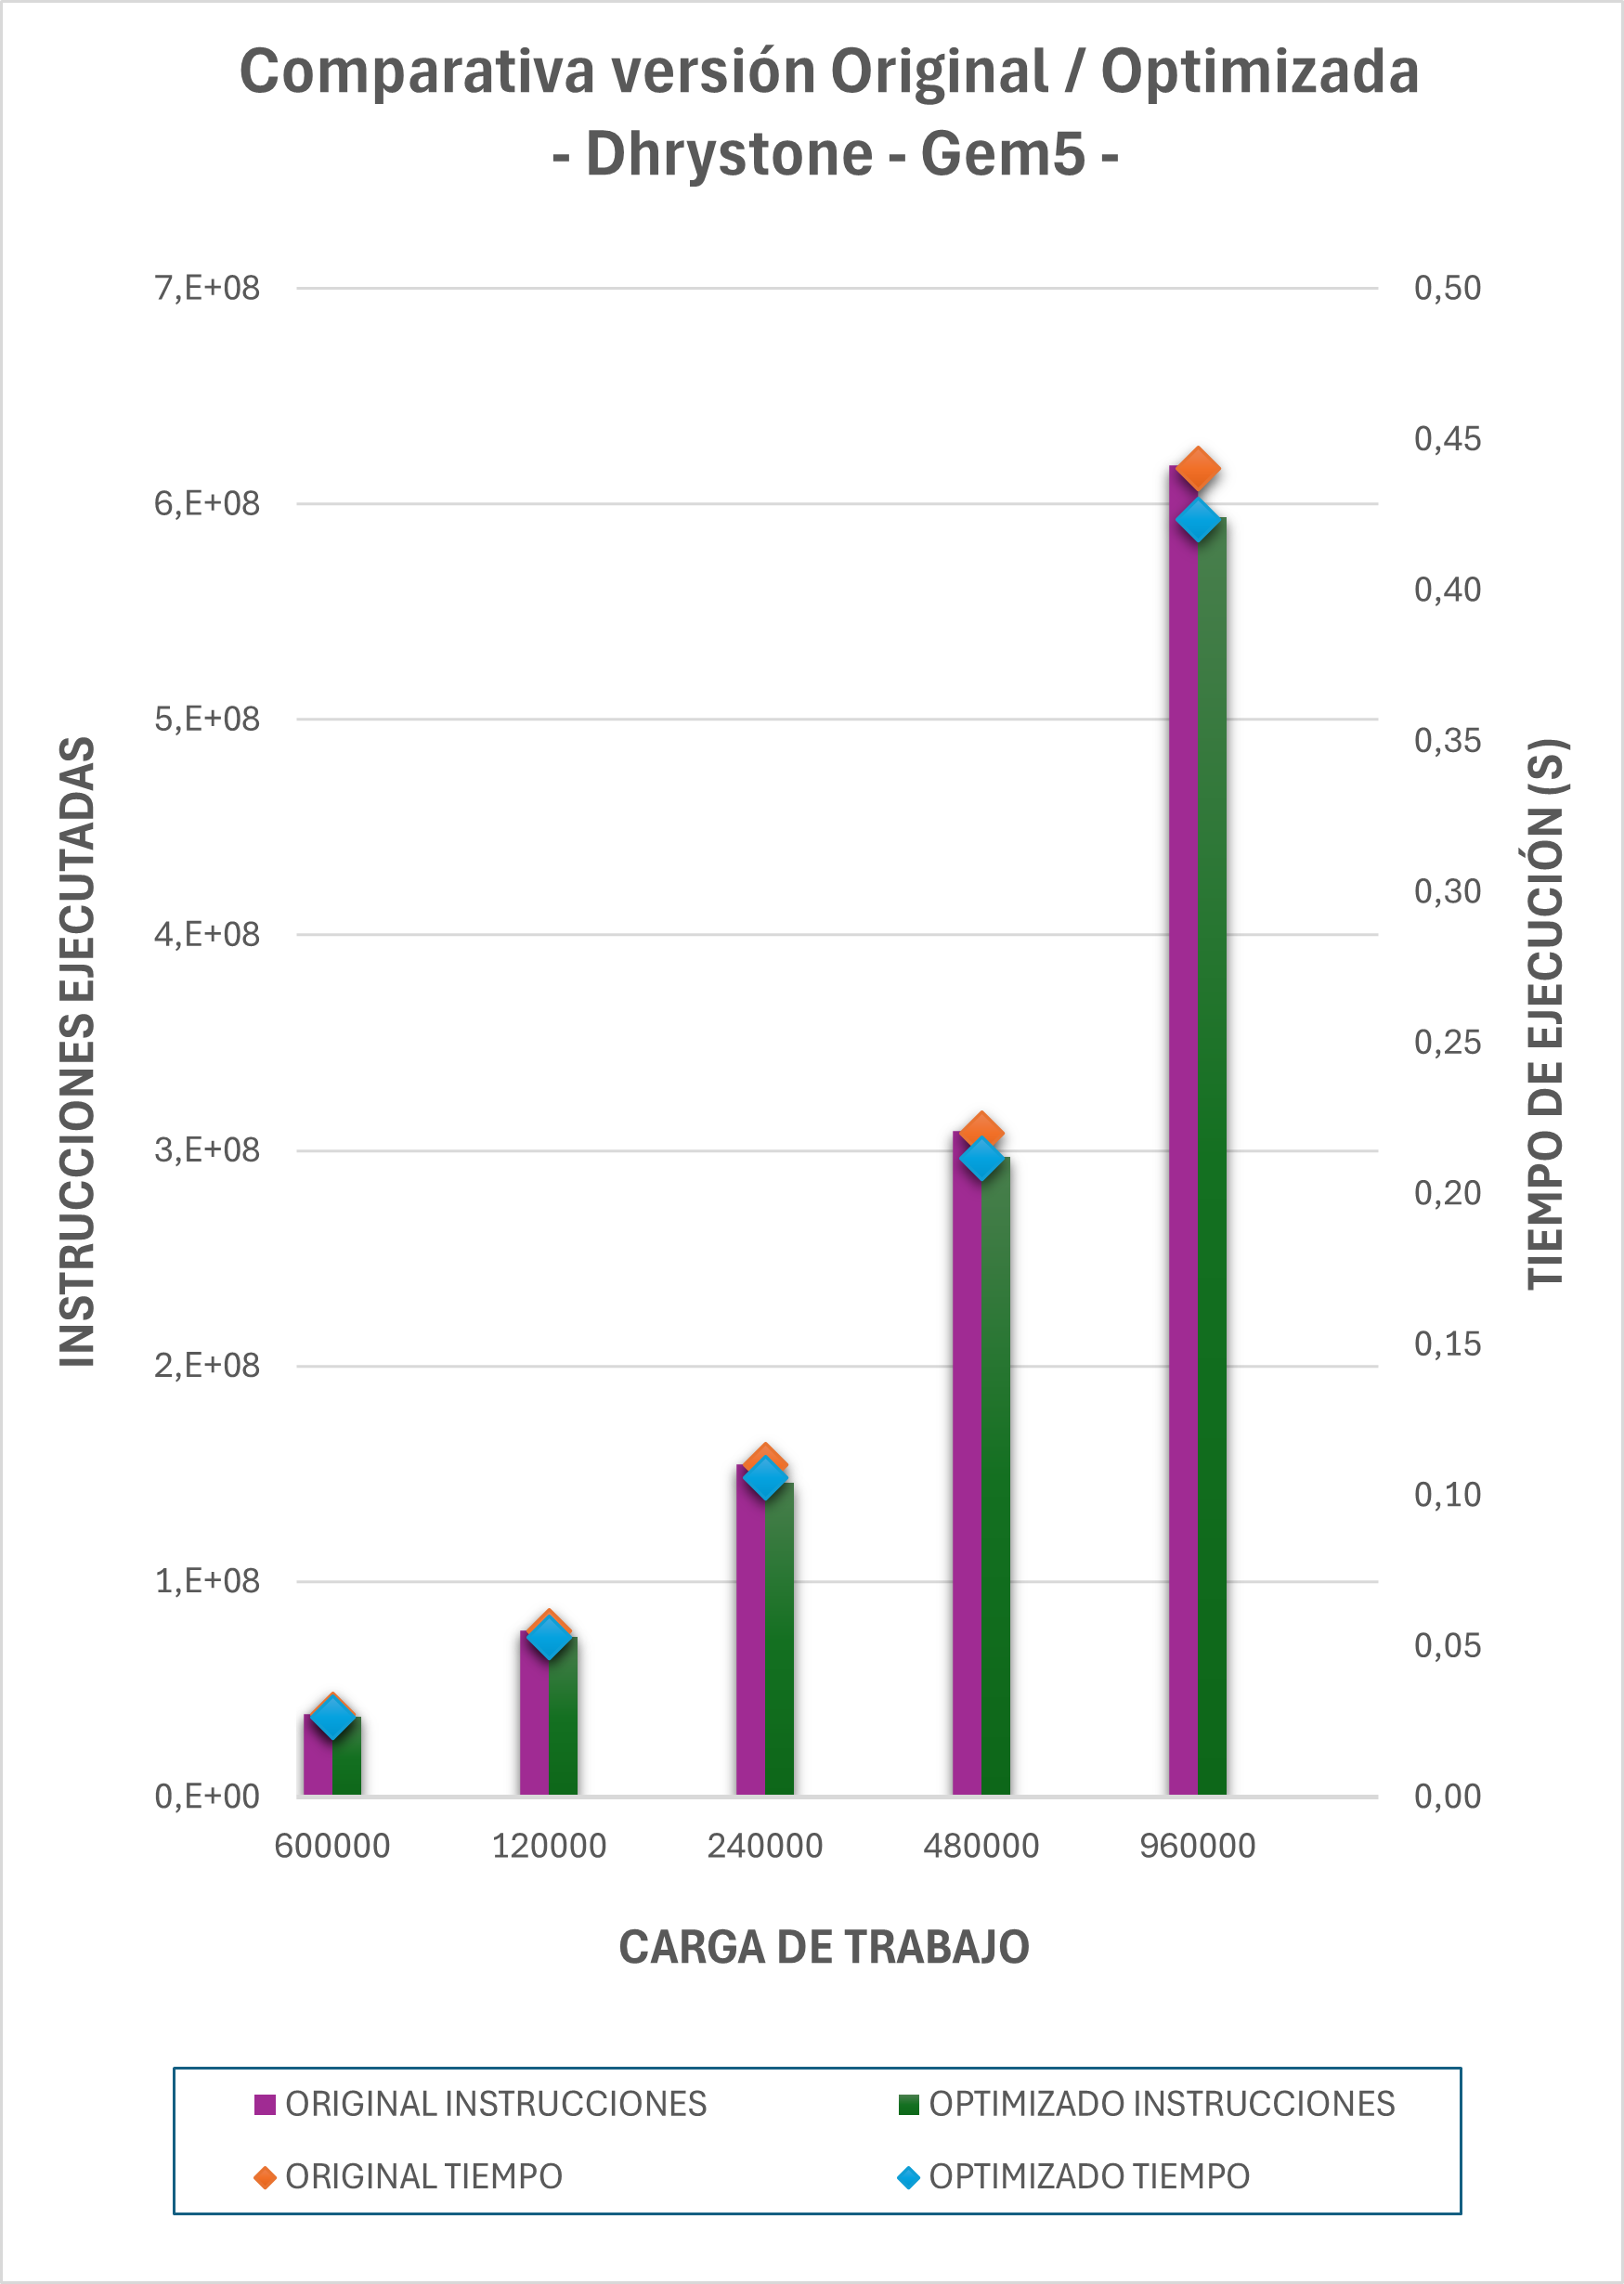
\includegraphics[width=0.95\linewidth, height=1.33\textwidth]{figs/dhrystoneGem5.png}
    \end{minipage}
    \begin{minipage}[b]{.48\textwidth}
    \centering
        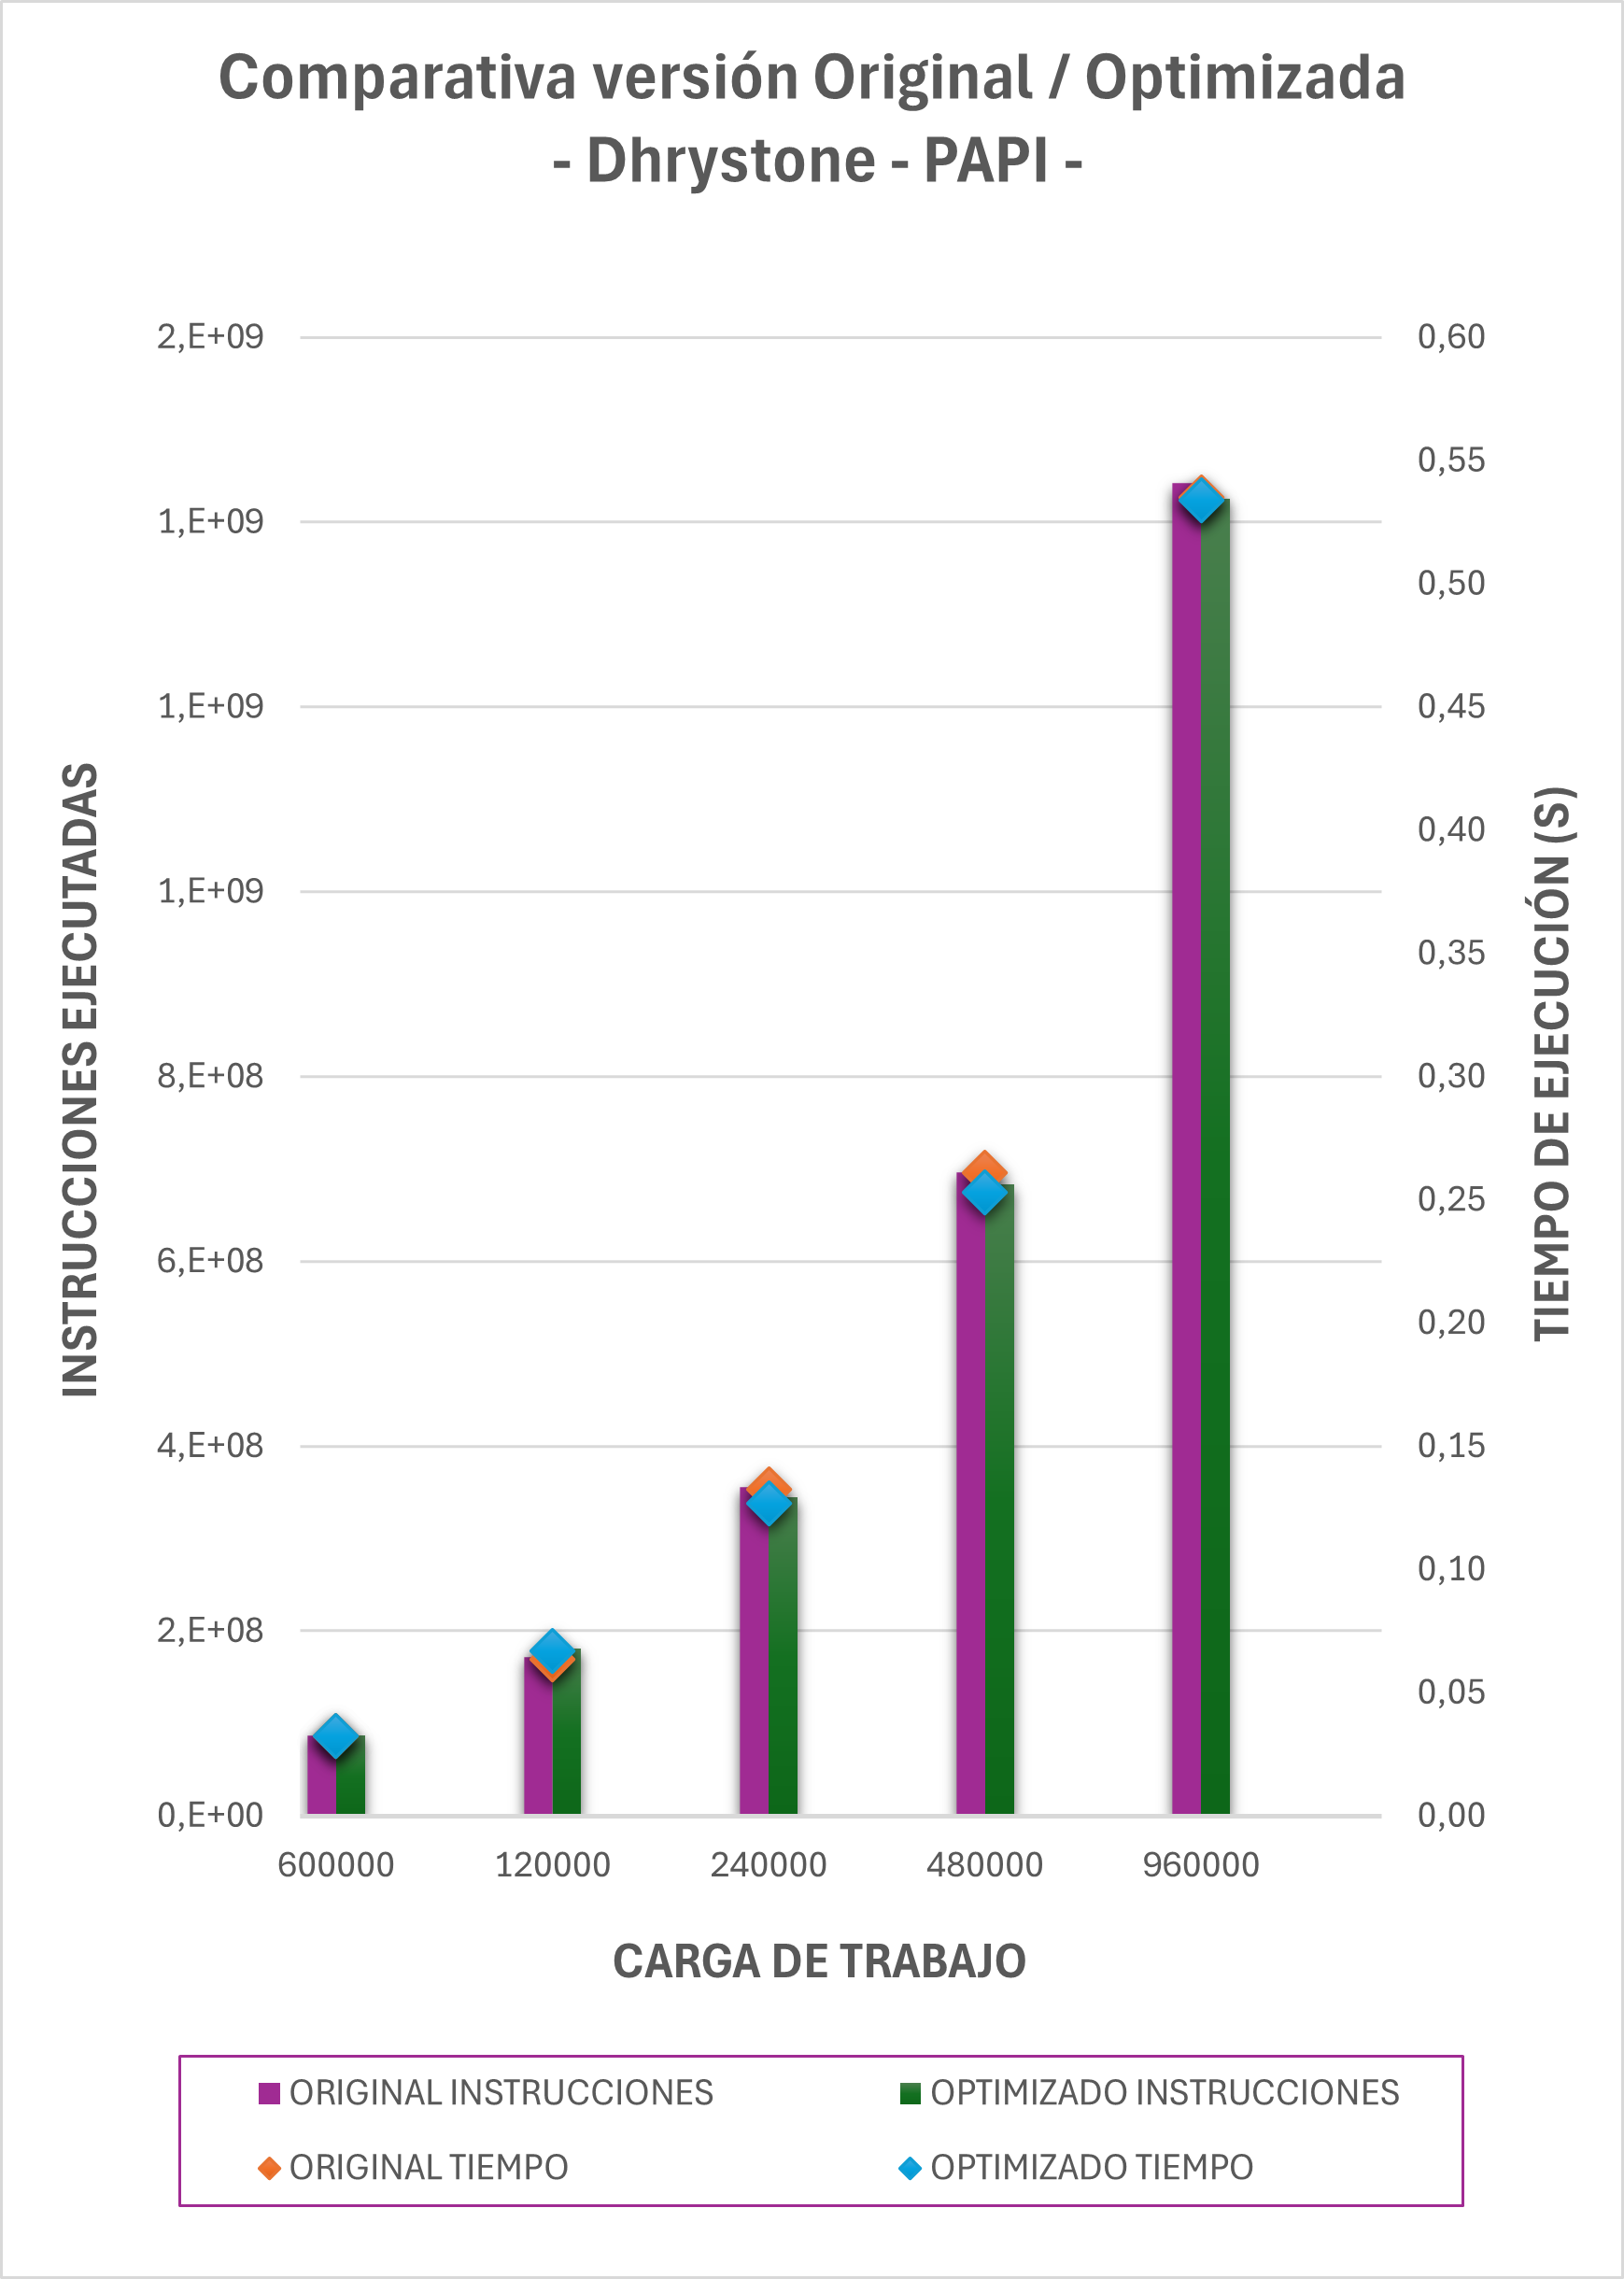
\includegraphics[width=0.95\linewidth, height=1.33\textwidth]{figs/dhrystonePAPI.png}
    \end{minipage}
    \caption{Comparativa versiones Dhrystone en Gem5 (izquierda) y PAPI (derecha)}
    \label{tab:optimizacionesDhrystone}
\end{figure}

La Figura~\ref{tab:optimizacionesDhrystone} muestra las mismas tendencias entre las instrucciones y el tiempo de ejecución de las diferentes cargas de trabajo, para ambas versiones del \textit{benchmark} Dhrystone, en PAPI y Gem5. Conforme crece la carga, el tiempo de ejecución y las instrucciones ejecutadas aumenta de forma proporcional. 

\paragraph{}
\label{conc:tiemposGem5PAPI}{
Sin embargo, como puede observarse en~\ref{tab:optimizacionesDhrystone} de la derecha, PAPI presenta unas métricas de instrucciones y tiempo dispares frente a los resultados de obtenidos con Gem5, algo que, en principio, no debería ser así. Esto se debe a que en la plataforma real se tienen unas latencias temporales, las cuales resultan complejas de modelar de forma precisa en Gem5, como por ejemplo, buses de interconexión, unidades funcionales, y memorias, ya que los componentes utilizados por la plataforma simulada en este trabajo no están modelados con la misma precisión, algo imposible de realizar en el plazo de este proyecto. Este aspecto hace que los tiempos en las simulaciones ejecutadas, al no tener unas latencias refinadas, entre otros aspectos, sean menores a los obtenidos en la plataforma física. En posteriores apartados se aborda esta problemática nuevamente.}

\subsection{Resultados}
\label{subs:obtencionResultados}

Para el marco de validación, es necesario tener en cuenta una serie de métricas relevantes para la caracterización del consumo, y que permitirán definir el modelo de consumo. En la tabla \ref{tab:resumenTablaMetodologia} y  se exponen los parámetros de \textit{hardware} y electricidad clave para caracterizar el consumo de energía, mientras que en la tabla \ref{tab:resumenTablaMetodologia2} se muestran los casos de uso seleccionados a la hora de ejecutar los \textit{benchmarks} seleccionados en este trabajo

\begin{table}[H]
\centering
\footnotesize
    \begin{tabular}{|ccc|}
    \hline
    \rowcolor[HTML]{9B9B9B} 
    \multicolumn{3}{|c|}{\cellcolor[HTML]{9B9B9B}\textbf{ MÉTRICAS RELEVANTES DE HARDWARE Y ELECTRICIDAD}}                                                                                          \\ \hline
    \rowcolor[HTML]{C0C0C0} 
    \multicolumn{2}{|c|}{\cellcolor[HTML]{C0C0C0}\textbf{ HARDWARE}}                                  & \textbf{ ELECTRICIDAD}                                                                       \\ \hline
    \multicolumn{1}{|c|}{ Número de ciclos}         & \multicolumn{1}{c|}{ Accesos totales Caché L1}   &  Potencia estática                                                                           \\ \hline
    \multicolumn{1}{|c|}{ Instrucciones ejecutadas} & \multicolumn{1}{c|}{ Fallos escritura Caché L1D} &  Potencia dinámica                                                                           \\ \hline
    \multicolumn{1}{|c|}{ Frecuencia componente}    & \multicolumn{1}{c|}{ Accesos lectura Caché L1D}  &                                                                                             \\ \cline{1-2}
    \multicolumn{1}{|c|}{ Voltaje componente}       & \multicolumn{1}{c|}{ Accesos totales Caché L2}   & \multirow{-2}{*}{\begin{tabular}[c]{@{}c@{}} Estimación de\\ energía consumida\end{tabular}} \\ \hline
    \end{tabular}
\caption{Métricas de \textit{hardware} (columnas 1 y 2) y electricidad (3) tenidas en cuenta en el trabajo}
\label{tab:resumenTablaMetodologia}
\end{table}

\begin{table}[H]
\centering
\footnotesize
    \begin{tabular}{|cccccc|}
    \hline
    \rowcolor[HTML]{C0C0C0} 
    \multicolumn{6}{|c|}{\cellcolor[HTML]{C0C0C0}\textbf{ESCENARIOS DE EJECUCIÓN DE  PROGRAMAS BENCHMARK}} \\ \hline
    \rowcolor[HTML]{EFEFEF} 
    \multicolumn{1}{|c|}{\cellcolor[HTML]{EFEFEF}\textbf{NOMBRE BENCHMARK}} & \multicolumn{5}{c|}{\cellcolor[HTML]{EFEFEF}\textbf{CARGAS DE TRABAJO}}                                                       \\ \hline
    \multicolumn{1}{|c|}{Dhrystone}                                         & \multicolumn{1}{c|}{60000}  & \multicolumn{1}{c|}{120000} & \multicolumn{1}{c|}{240000}  & \multicolumn{1}{c|}{480000}  & 960000  \\ \hline
    \multicolumn{1}{|c|}{Whetstone}                                         & \multicolumn{1}{c|}{3000}   & \multicolumn{1}{c|}{6000}   & \multicolumn{1}{c|}{12000}   & \multicolumn{1}{c|}{24000}   & 48000   \\ \hline
    \multicolumn{1}{|c|}{Cálculo de decimales número Pi}                    & \multicolumn{1}{c|}{300000} & \multicolumn{1}{c|}{600000} & \multicolumn{1}{c|}{1200000} & \multicolumn{1}{c|}{2400000} & 4800000 \\ \hline
    \multicolumn{1}{|c|}{Cálculo de números primos}                         & \multicolumn{1}{c|}{3000}   & \multicolumn{1}{c|}{6000}   & \multicolumn{1}{c|}{12000}   & \multicolumn{1}{c|}{24000}   & 48000   \\ \hline
    \end{tabular}
\caption{Configuraciones tenidas en cuenta durante la ejecución de los programas \textit{benchmark}}
\label{tab:resumenTablaMetodologia2}
\end{table} 

Tras la ejecución de los programas, se han agrupado las métricas que consideradas de gran relevancia a nivel energético, ya explicadas en este \ac{TFM}, tanto para Gem5 como para PAPI. En las figuras \ref{fig:tablaDhrystoneGem5}, \ref{fig:tablaWhetstoneGem5}, \ref{fig:tablaCalcpiGem5}, \ref{fig:tablaCalcprimosGem5} se presentan los resultados para Gem5. En estas tablas se han utilizado abreviaturas; para evitar confusiones, se muestra en la figura \ref{fig:abreviaturas} el significado de cada una. 

\begin{table}[H]
    \footnotesize
    \centering
    \begin{tabular}{|
        >{\columncolor[HTML]{C0C0C0}}c 
        >{\columncolor[HTML]{FFFFFF}}c 
        >{\columncolor[HTML]{C0C0C0}}c 
        >{\columncolor[HTML]{FFFFFF}}c |}
        \hline
        \multicolumn{4}{|c|}{\cellcolor[HTML]{9B9B9B}\textbf{SIGNIFICADO DE LAS ABREVIATURAS}}                                                                                                                                                                                                                                     \\ \hline
        \multicolumn{1}{|c|}{\cellcolor[HTML]{C0C0C0}\textbf{ABREV.}} & \multicolumn{1}{c|}{\cellcolor[HTML]{FFFFFF}\textbf{DESCRIPCIÓN}}                         & \multicolumn{1}{c|}{\cellcolor[HTML]{C0C0C0}\textbf{ABREV.}}      & \textbf{DESCRIPCIÓN}                                                             \\ \hline
        \multicolumn{1}{|c|}{\cellcolor[HTML]{C0C0C0}CICLOS}               & \multicolumn{1}{c|}{\cellcolor[HTML]{FFFFFF}Número de ciclos de ejecución}                & \multicolumn{1}{c|}{\cellcolor[HTML]{C0C0C0}V}                         & Voltaje del componente procesador                                                \\ \hline
        \multicolumn{1}{|c|}{\cellcolor[HTML]{C0C0C0}AT-L1}                & \multicolumn{1}{c|}{\cellcolor[HTML]{FFFFFF}Accesos totales caché L1}                     & \multicolumn{1}{c|}{\cellcolor[HTML]{C0C0C0}ATD-L1}                    & Accesos totales caché L1 de datos                                                \\ \hline
        \multicolumn{1}{|c|}{\cellcolor[HTML]{C0C0C0}INSTR-TOT}            & \multicolumn{1}{c|}{\cellcolor[HTML]{FFFFFF}Instrucciones totales ejecutadas}             & \multicolumn{1}{c|}{\cellcolor[HTML]{C0C0C0}ATI-L1}                    & Accesos totales caché L1 de instrucciones                                        \\ \hline
        \multicolumn{1}{|c|}{\cellcolor[HTML]{C0C0C0}INSTR-ALU}            & \multicolumn{1}{l|}{\cellcolor[HTML]{FFFFFF}Intrucciones de cálculo de entero y flotante} & \multicolumn{1}{c|}{\cellcolor[HTML]{C0C0C0}AT-L2}                     & Accesos totales caché L2                                                         \\ \hline
        \multicolumn{1}{|c|}{\cellcolor[HTML]{C0C0C0}FPE-L1}               & \multicolumn{1}{l|}{\cellcolor[HTML]{FFFFFF}Fallos en peticiones de escritura caché L1}   & \multicolumn{1}{c|}{\cellcolor[HTML]{C0C0C0}T (s)}                     & Tiempo de ejecución, en segundos                                                 \\ \hline
        \multicolumn{1}{|c|}{\cellcolor[HTML]{C0C0C0}APL-L1}               & \multicolumn{1}{l|}{\cellcolor[HTML]{FFFFFF}Aciertos en peticiones de lectura caché L1}   & \multicolumn{1}{c|}{\cellcolor[HTML]{C0C0C0}}                          & \cellcolor[HTML]{FFFFFF}                                                         \\ \cline{1-2}
        \multicolumn{1}{|c|}{\cellcolor[HTML]{C0C0C0}FEAPL-L1}             & \multicolumn{1}{c|}{\cellcolor[HTML]{FFFFFF}Combinación de las dos métricas de arriba}    & \multicolumn{1}{c|}{\multirow{-2}{*}{\cellcolor[HTML]{C0C0C0}T-M (s)}} & \multirow{-2}{*}{\cellcolor[HTML]{FFFFFF}Tiempo de ejecución medio, en segundos} \\ \hline
    \end{tabular}
    \caption{Significado de las abreviaturas utilizadas en las figuras tras realizar las ejecuciones}
    \label{fig:abreviaturas}
\end{table}

\begin{figure}[H]
    \centering
    \resizebox{1\linewidth}{1.2\textwidth}{
    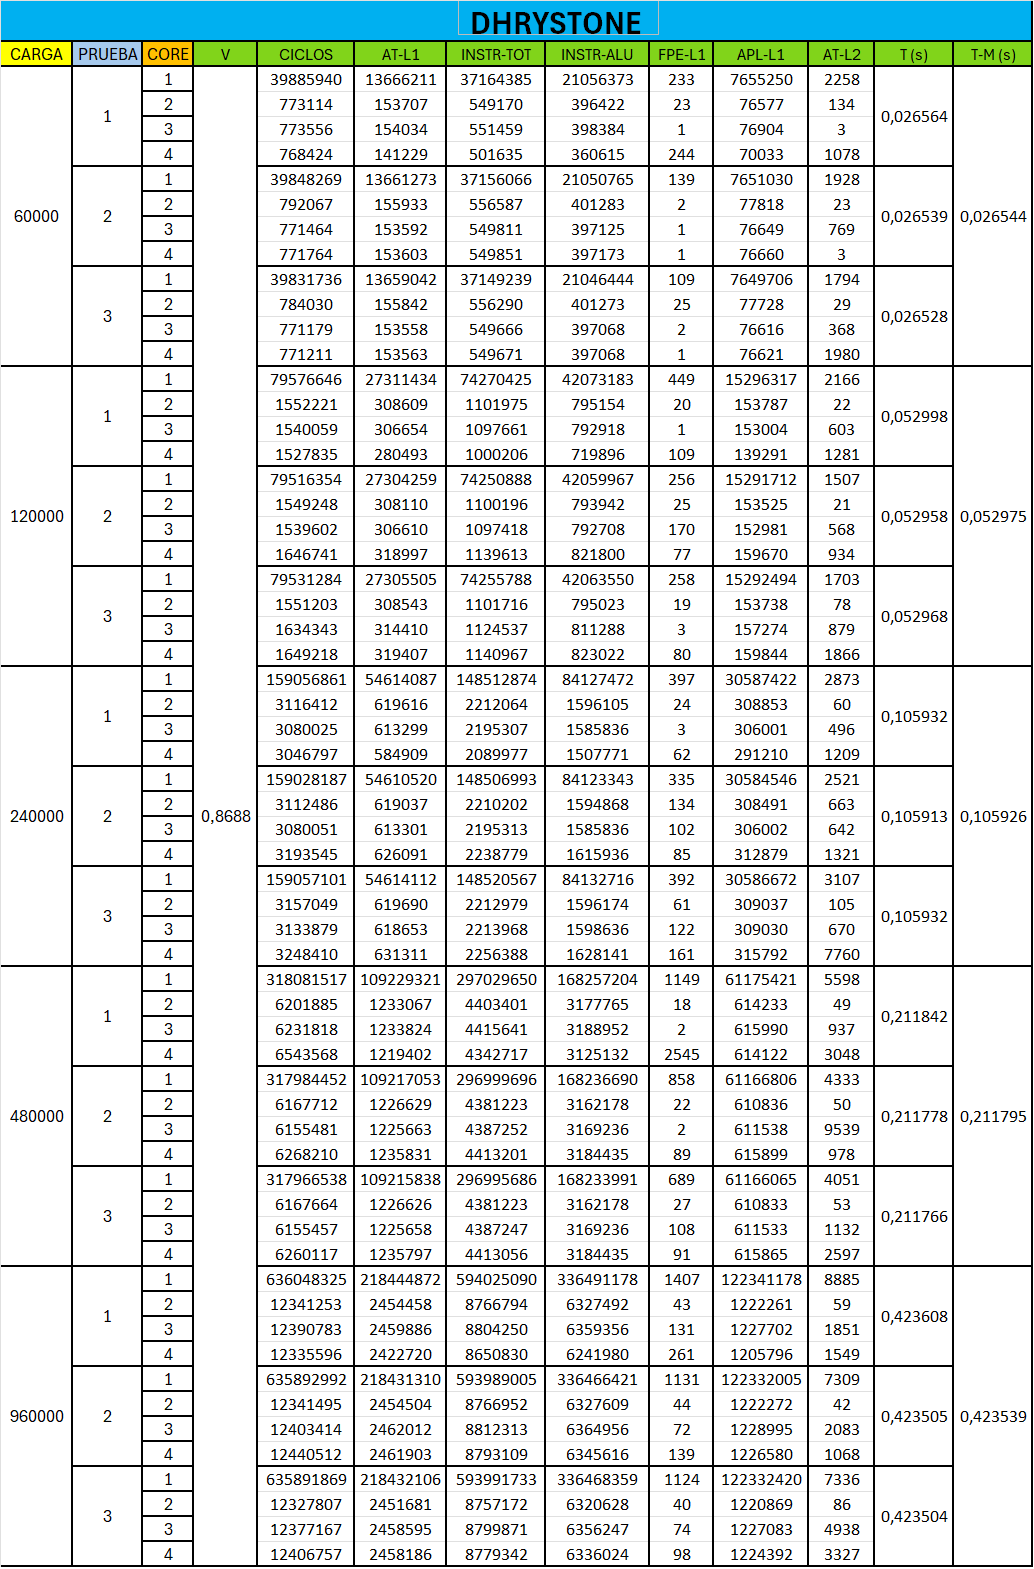
\includegraphics{figs/metricas_dhrystone.png}}
    \caption{Métricas obtenidas del \textit{benchmark} Dhrystone en Gem5}
    \label{fig:tablaDhrystoneGem5}
\end{figure}

\begin{figure}[H]
    \centering
    \resizebox{1\linewidth}{1.2\textwidth}{
    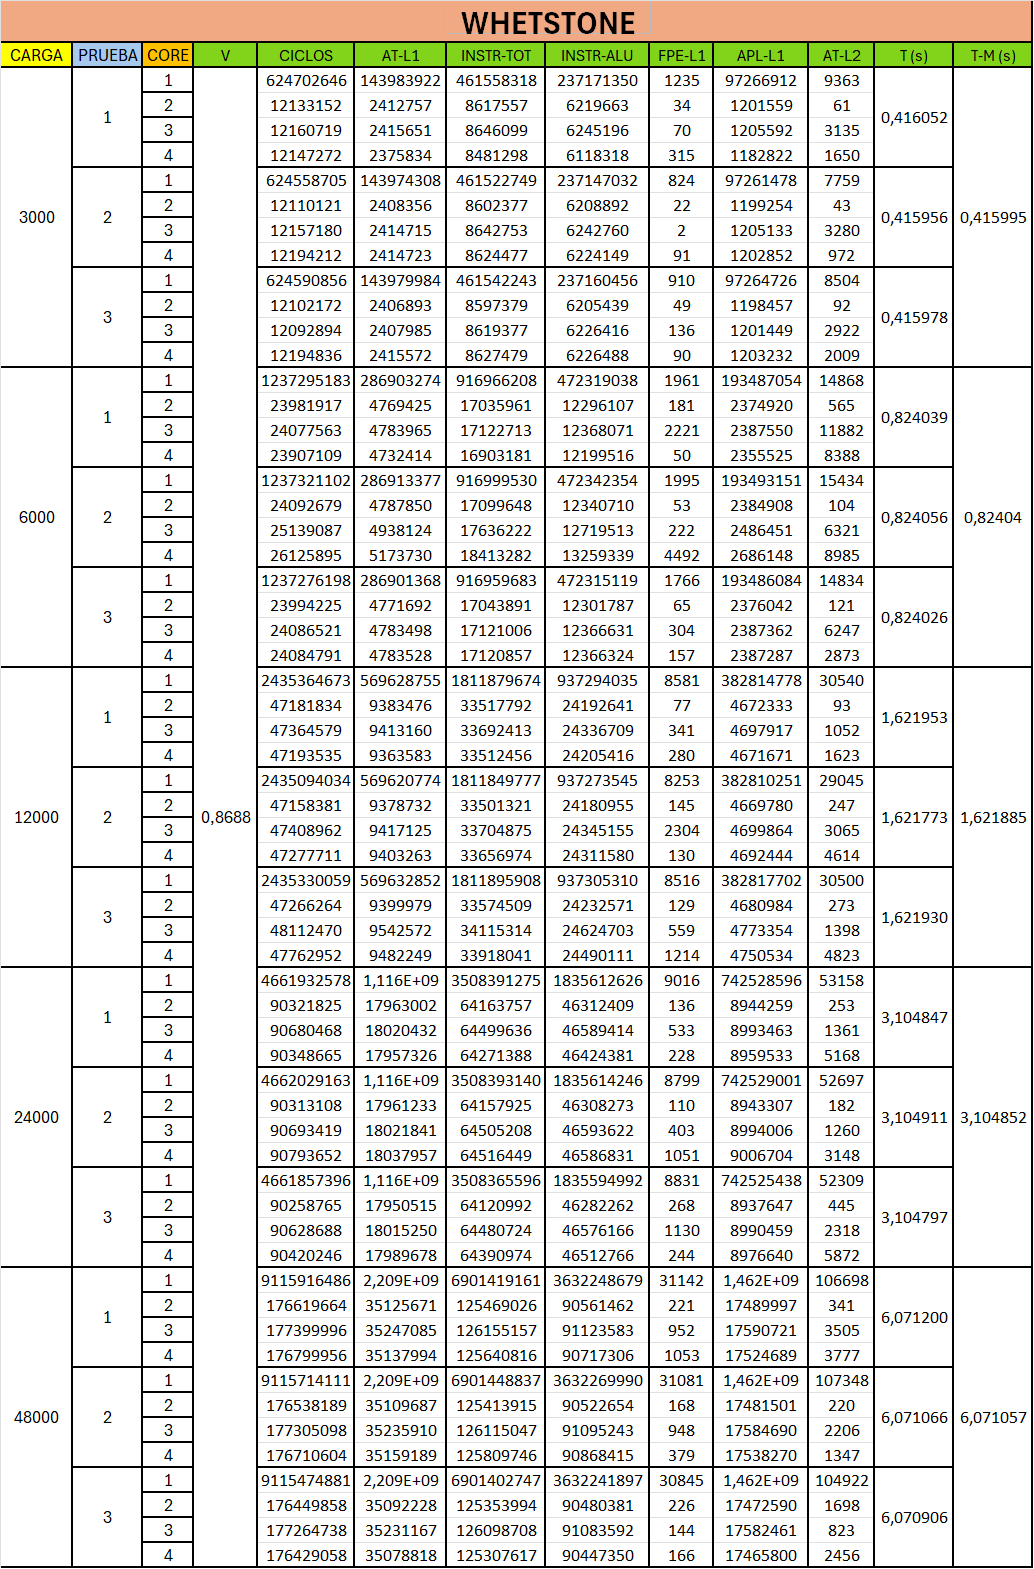
\includegraphics{figs/metricas_whetstone.png}}
    \caption{Métricas obtenidas del \textit{benchmark} Whetstone en Gem5}
    \label{fig:tablaWhetstoneGem5}
\end{figure}
    
\begin{figure}[H]
    \centering
    \resizebox{1\linewidth}{1.2\textwidth}{
    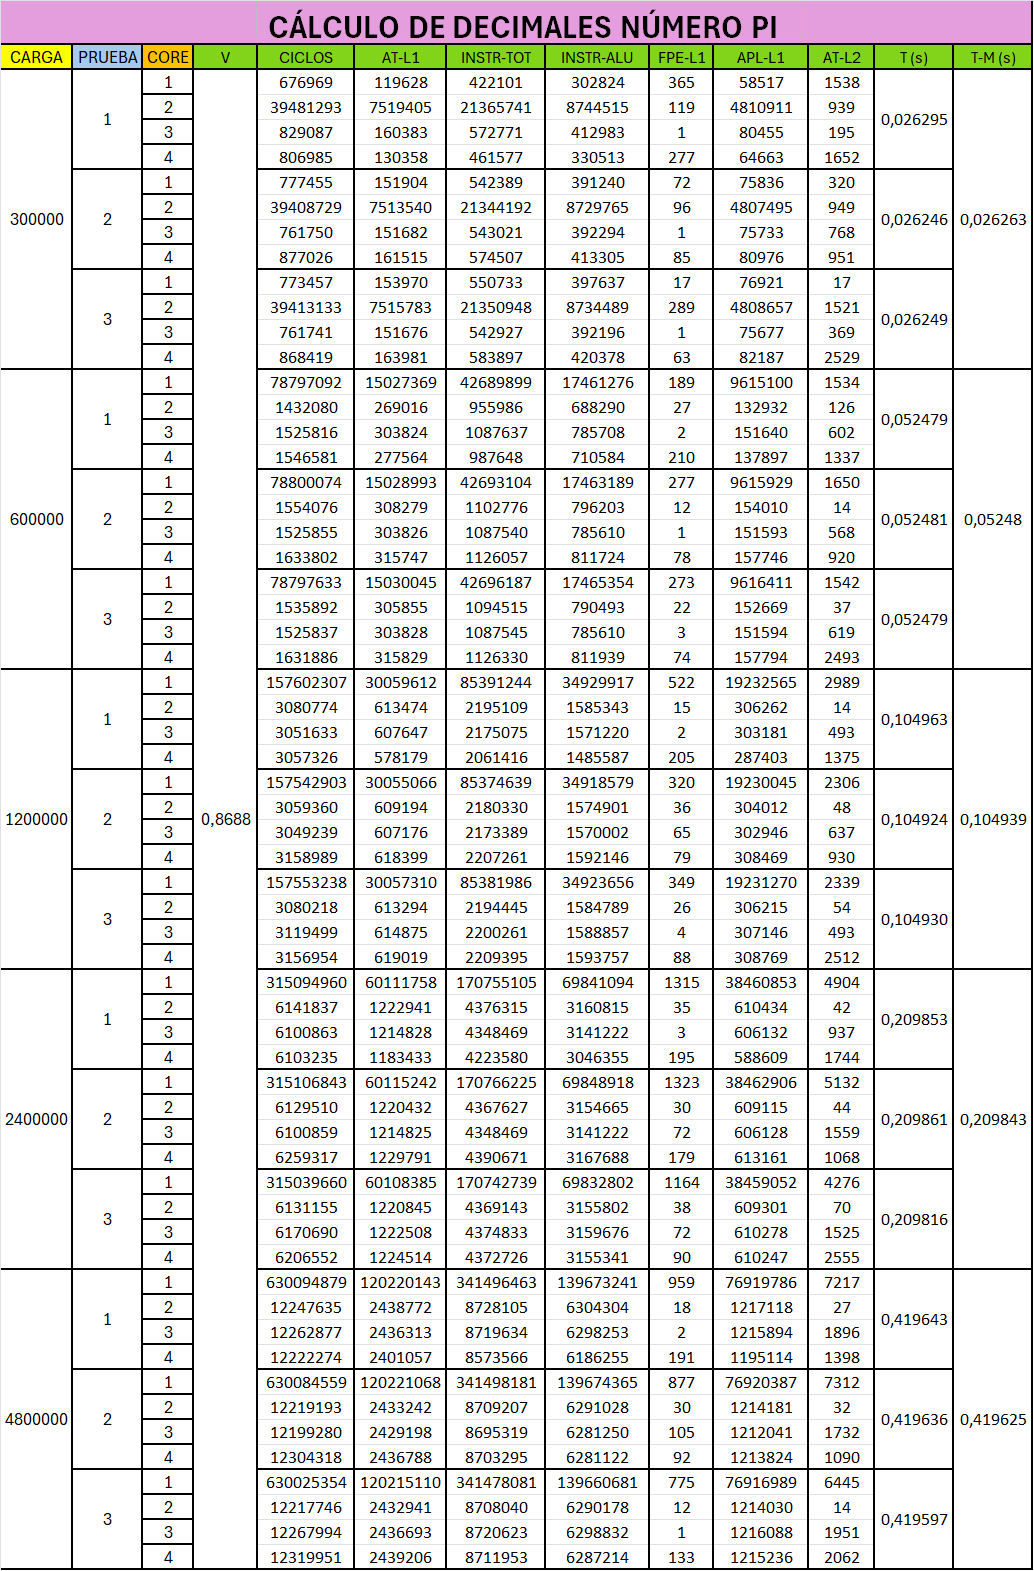
\includegraphics{figs/metricas_calcpi.png}}
    \caption{Métricas obtenidas del \textit{benchmark} Cálculo de Pi en Gem5}
    \label{fig:tablaCalcpiGem5}
\end{figure}

\begin{figure}[H]
    \centering
    \resizebox{1\linewidth}{1.2\textwidth}{
    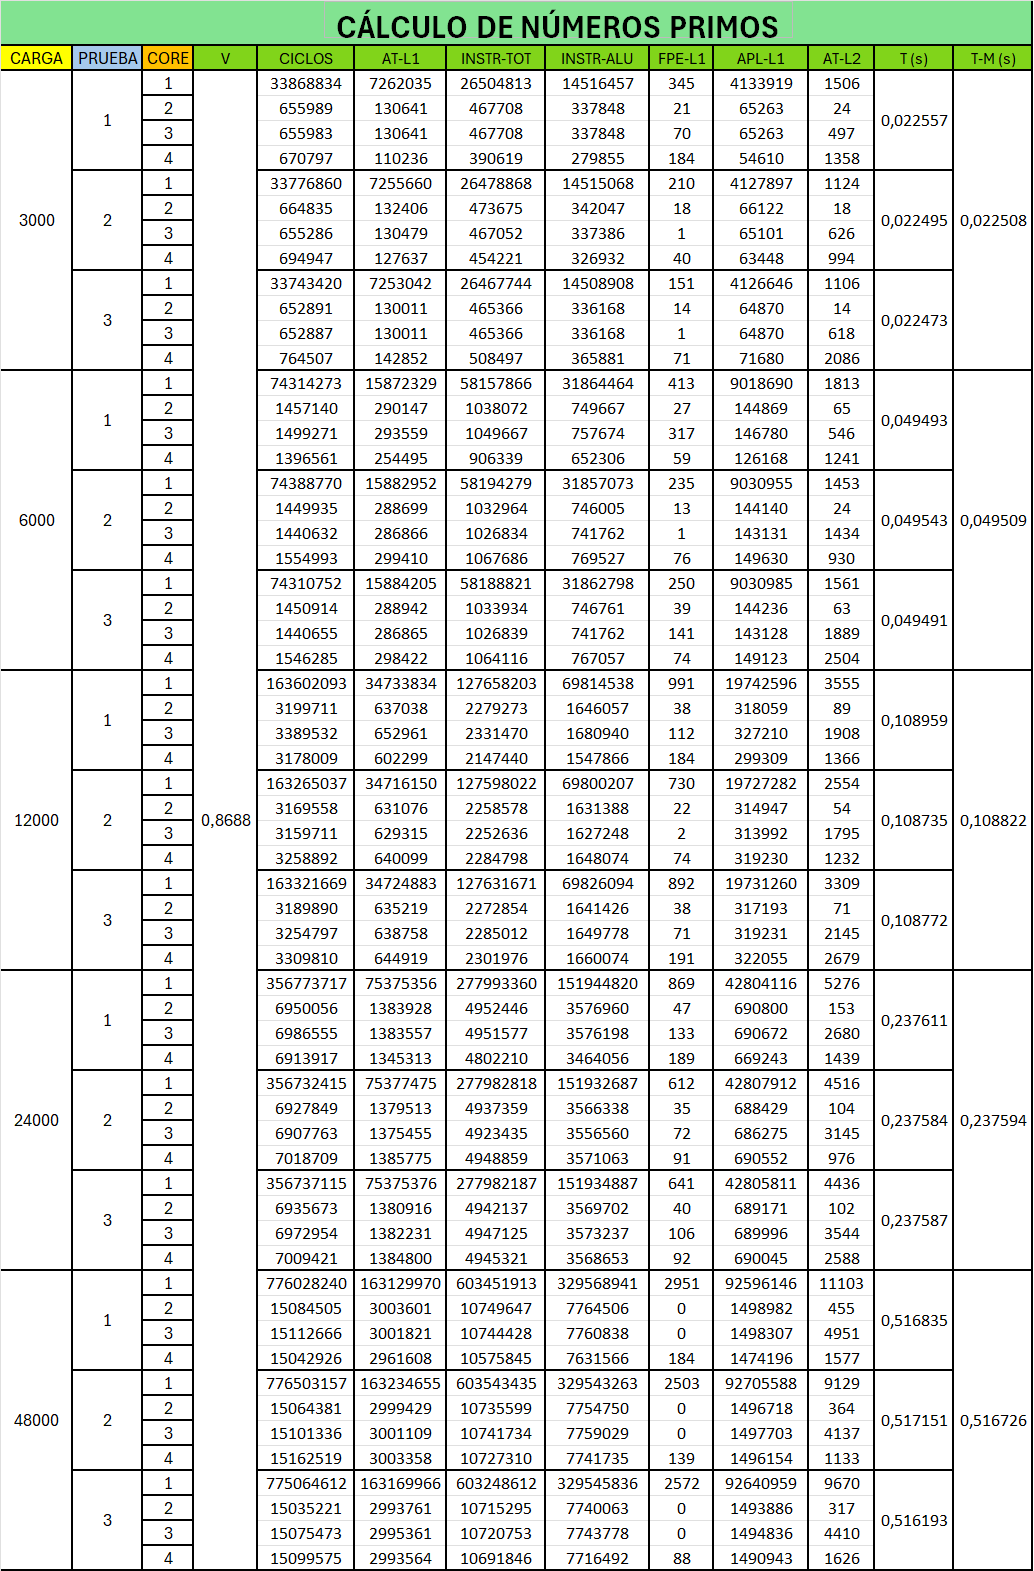
\includegraphics{figs/metricas_calcprimos.png}}
    \caption{Métricas obtenidas del \textit{benchmark} Cálculo de números primos en Gem5}
    \label{fig:tablaCalcprimosGem5}
\end{figure}

Como puede observarse en las figuras \ref{fig:tablaDhrystoneGem5}, \ref{fig:tablaWhetstoneGem5}, \ref{fig:tablaCalcpiGem5} y \ref{fig:tablaCalcprimosGem5}, todos los programas \textit{benchmark}, para todas las cargas de trabajo, se ejecutan de forma secuencial. Prueba de ello son los valores de las tablas para cada \textit{core} en cada una de las ejecuciones realizadas: en todas ellas, uno de los \textit{cores} se emplea a fondo, mientras que el resto se mantienen inactivos. Además, se puede apreciar que, conforme suben las cargas de trabajo, los tiempos de ejecuión aumentan de forma lineal. En \ref{fig:tablaMetricasPAPI} se muestran los resultados obtenidos por PAPI, utilizando abreviaturas de nuevo, pudiéndose ver el significado de éstas en \ref{fig:abreviaturas}.

\begin{figure}[H]
    \centering
    \resizebox{1\linewidth}{1.3\textwidth}{
    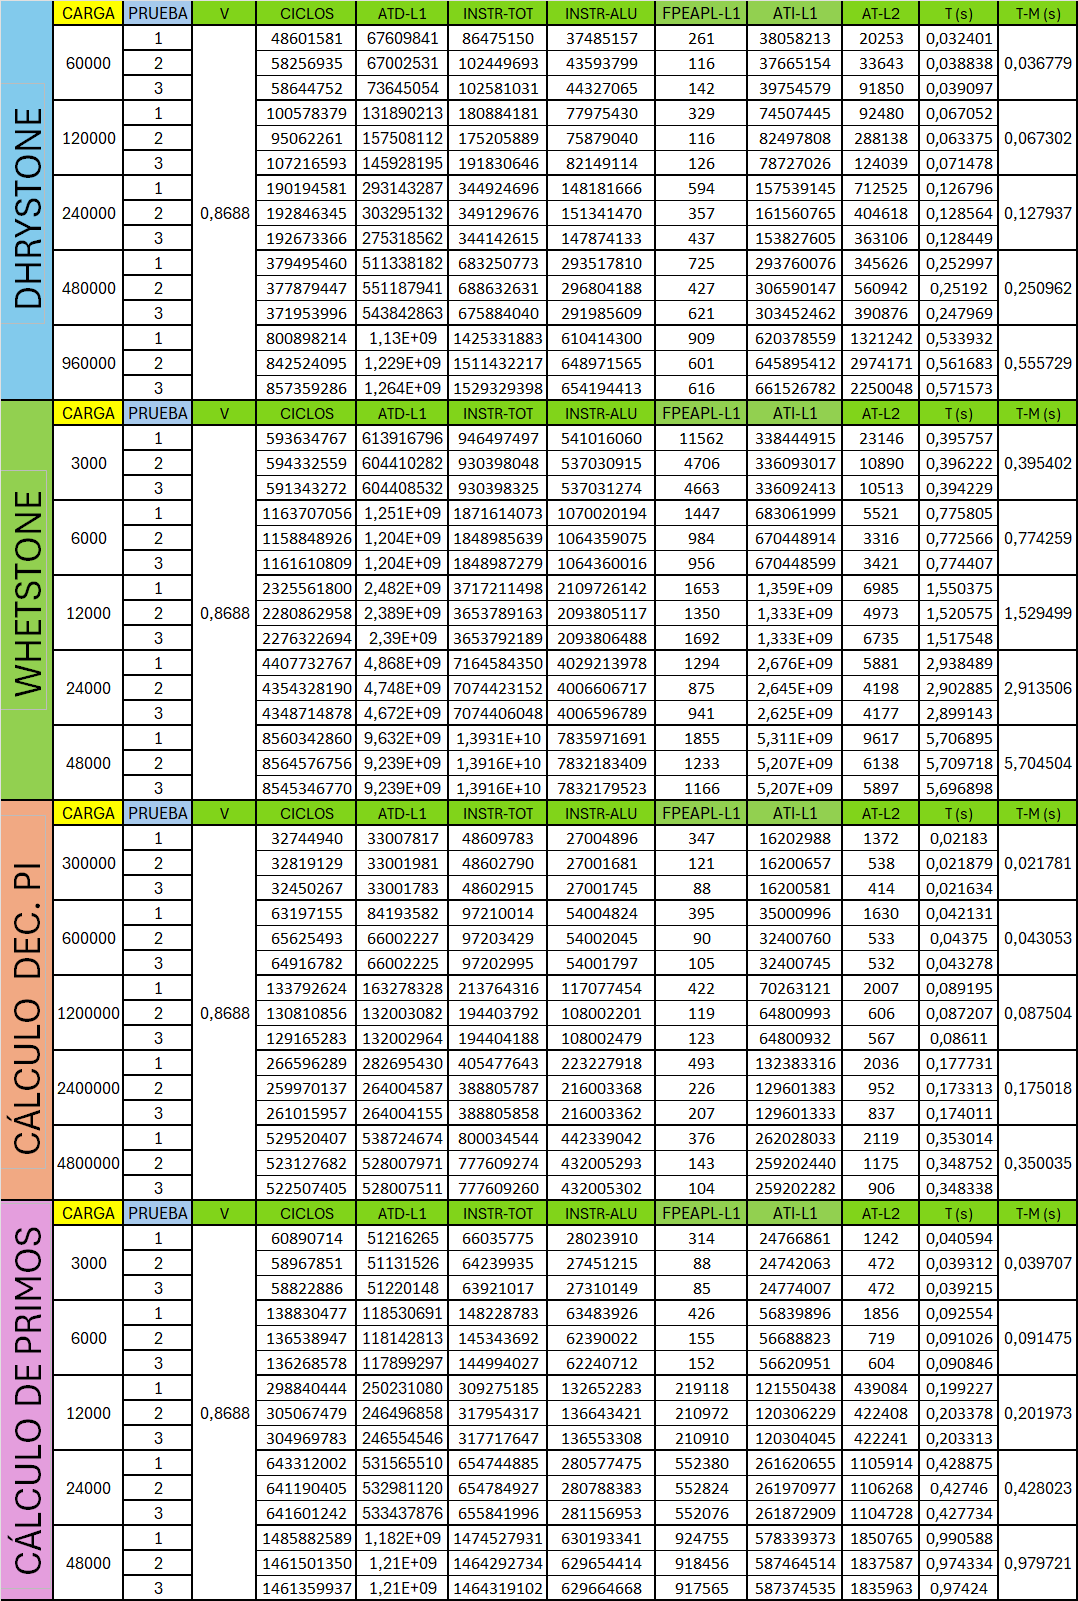
\includegraphics{figs/metricas-papi.png}}
    \caption{Métricas obtenidas de los \textit{benchmark} en PAPI}
    \label{fig:tablaMetricasPAPI}
\end{figure}

Como puede observarse en \ref{fig:tablaMetricasPAPI}, en las ejecuciones con PAPI no se tienen varios \textit{cores}, representando cada ejecución una única fila, la cual representa al \textit{core} que ha ejecutado cada \textit{benchmark}, debido a la naturaleza secuencial de todos los programas escogidos para este proyecto. Al igual que sucedía con los resultados de Gem5, conforme sube las cargas de trabajo, los tiempos de ejecuión aumentan de la misma manera. 

Para poder realizar una comparativa de resultados entre ambos escenarios, se muestran en la figura \ref{fig:diferenciaTiemposCaches} las diferencias medias relativas de Gem5 sobre PAPI en casos concretos, como el tiempo de ejecución y métricas obtenidas de las cachés. Nuevamente, para mantener el estilo de las tablas, se han empleado abreviaturas, pudiéndose ver el significado de éstas en \ref{fig:abreviaturas}.

\begin{figure}[H]
    \centering
    \resizebox{0.95\linewidth}{0.75\textwidth}{
    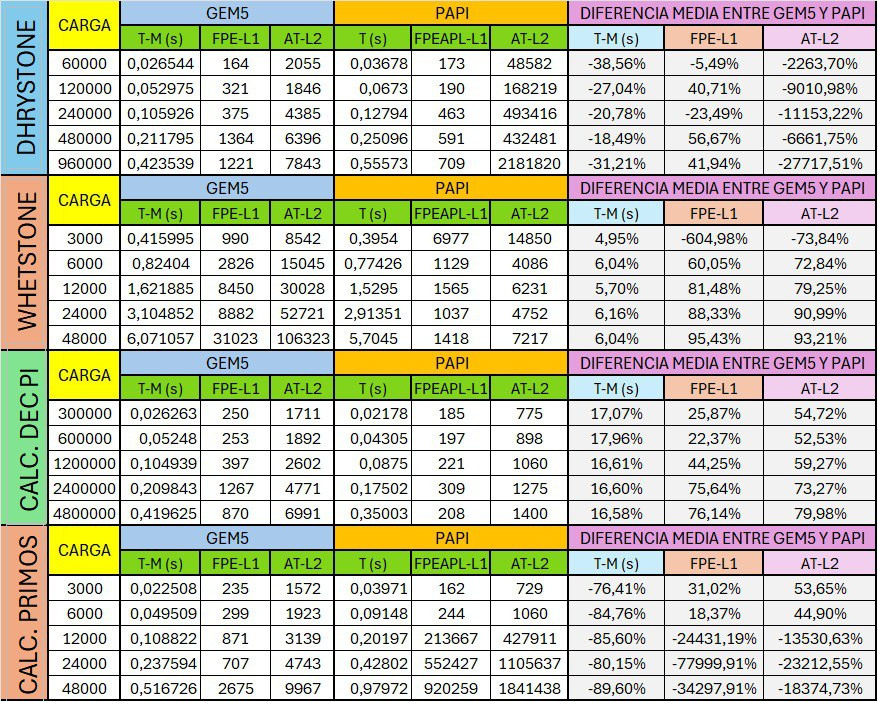
\includegraphics{figs/diferenciaTiemposCaches.jpg}}
    \caption{Comparativa de resultados de tiempos de ejecución y cahés en Gem5 y PAPI}
    \label{fig:diferenciaTiemposCaches}
\end{figure}

El análisis de estos resultados ha proporcionado las siguientes conclusiones:

\begin{enumerate}%[noitemsep]
    \item \textbf{Los \textit{benchmarks} intensivos en \ac{FPU} están mejor modelados en Gem5 que aquellos intensivos en ALU}: los tiempos de simulación en Gem5 y los obtenidos con PAPI demuestran que los \textit{benchmarks} Whetstone y Cálculo de decimales del número Pi, que utilizan de forma intensiva las FPU, presentan unas diferencias de tiempo menores. En ellos, los tiempos de simulación son incluso mayores al real, dando la sensación de un buen modelado de esta unidad. En ejecutar Whetstone, Gem5 un 6.16\% más como máximo, siendo el máximo para el Cálculo de decimales de Pi un 17.96\%. No puede decirse lo mismo de aquellos \textit{benchmarks} intensivos en \ac{ALU}, donde las diferencias son incluso negativas, lo que representa un mayor tiempo de ejecución en la versión de PAPI frente a la de Gem5, alcanzándose un 38.56\% menos de tiempo en Dhrystone y un 89.90\% menos en el Cálculo de números primos.

    \item \textbf{Los valores de fallos de escritura en Gem5 para el componente caché L1 son inconsistentes}: como puede observarse en las columnas $FPE-L1$ y $FPEAPL-L1$, para Gem5 y PAPI, respectivamente, se tiene un mayor número de fallos en PAPI que en Gem5, presentándose inconsistencias importantes ante ciertos escenarios, destacando un 24431.19\% menos en Gem5 al computar 12000 números primos, un 77999.91\% menos para 24000, y un 34297\% menos para 48000. Esto es debido a que, a la hora de cálcular la primalidad dentro de un gran conjunto de números, mediante el algoritmo de Miller-Rabin, se tiene que tener cierta cantidad de valores recientemente probados en memoria caché para asegurar la primalidad. Esto provoca la necesidad de realizar reemplazos de forma periódica, siendo clave una política de reemplazo en caché eficiente, para evitar fallos. Estos resultados muestran una baja fidelidad en el modelado de la caché L1, destacando imprecisiones en las políticas de reemplazo e interconexiones utilizadas en el simulador frente a la plataforma de cómputo real: según \cite{gem5-cache}, en Gem5, la caché L1 está conectada por un bus de barras cruzadas, y la política de reemplazo es, por defecto Least Recently Used (LRU); sin embargo, por el contrario, no se ha logrado averiguar ni la política de reemplazo ni el tipo de interconexión de la plataforma de cómputo utilizada. Esta problemática tiene, por tanto, difícil solución con la información actual.

    \item \textbf{Existe una gran diferencia en los accesos totales a la caché L2}: como se observa en la columna $AT-L2$ para Gem5 y PAPI, en Dhrystone y Cálculo de números primos existe una diferencia máxima de un 27717.51\% menos y un 23212.55\% menos en Gem5 para los respectivos \textit{benchmarks}, quedando, por tanto, los accesos totales de caché L2 en PAPI muy por encima de Gem5; sin embargo, para los \textit{benchmarks} intensivos en \ac{FPU}, no se tiene la misma problemática, obteniéndose diferencias de máximo un 93.21\% más en Gem5 para Whetstone y un 79.98\% superior para el Cálculo de decimales de Pi. Este comportamiento variable sucede por potenciales imprecisiones a la hora de modelar el componente caché L2, las cuales, según el tipo de \textit{benchmark}, tendrán una mayor o menor importancia. Esto es una problemática compleja de solucionar, debido a los plazos de este proyecto.
\end{enumerate}

Para finalizar, se ha calculado la potencia total (dinámica más estática) para Gem5 y PAPI con las fórmulas y descripciones mostradas en \ref{mostrandoModelos} y \ref{explicacionModelos}. En las figuras \ref{fig:potenciaGem5} y \ref{fig:potenciaPAPI} se muestran los resultados de potencia total para cada carga de trabajo de cada \textit{benchmark} seleccionado dentro de este trabajo.

\begin{figure}[H]
    \centering
    \resizebox{0.85\linewidth}{0.45\textwidth}{
    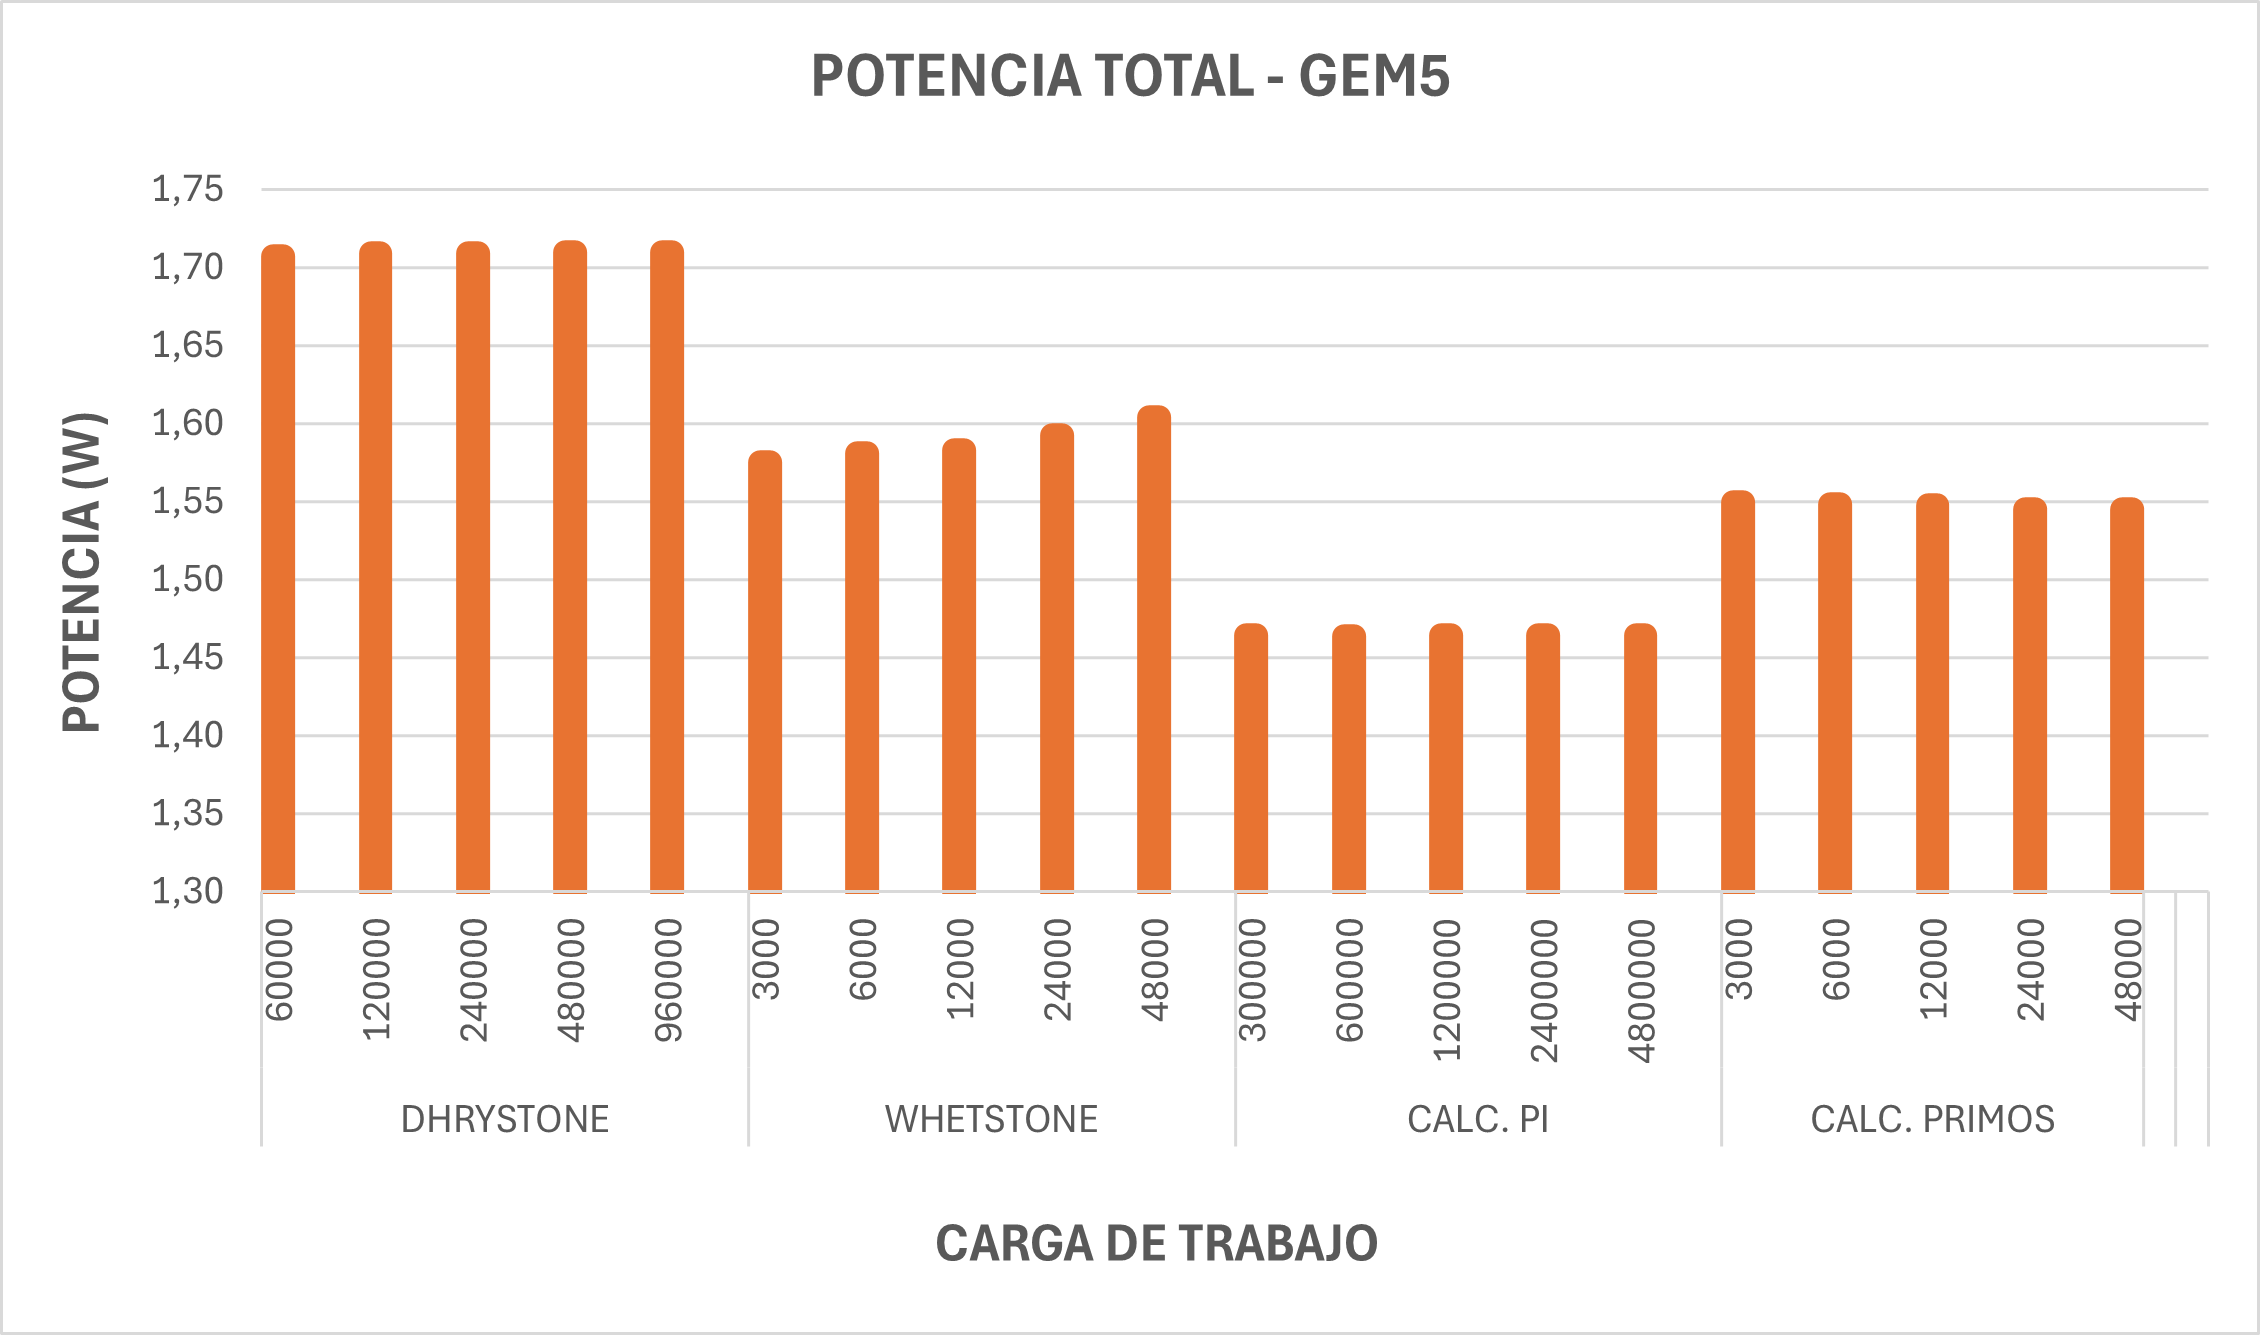
\includegraphics{figs/potenciaGem5.png}}
    \caption{Potencia total de los \textit{benchmark} en Gem5}
    \label{fig:potenciaGem5}
\end{figure}

\begin{figure}[H]
    \centering
    \resizebox{0.85\linewidth}{0.45\textwidth}{
    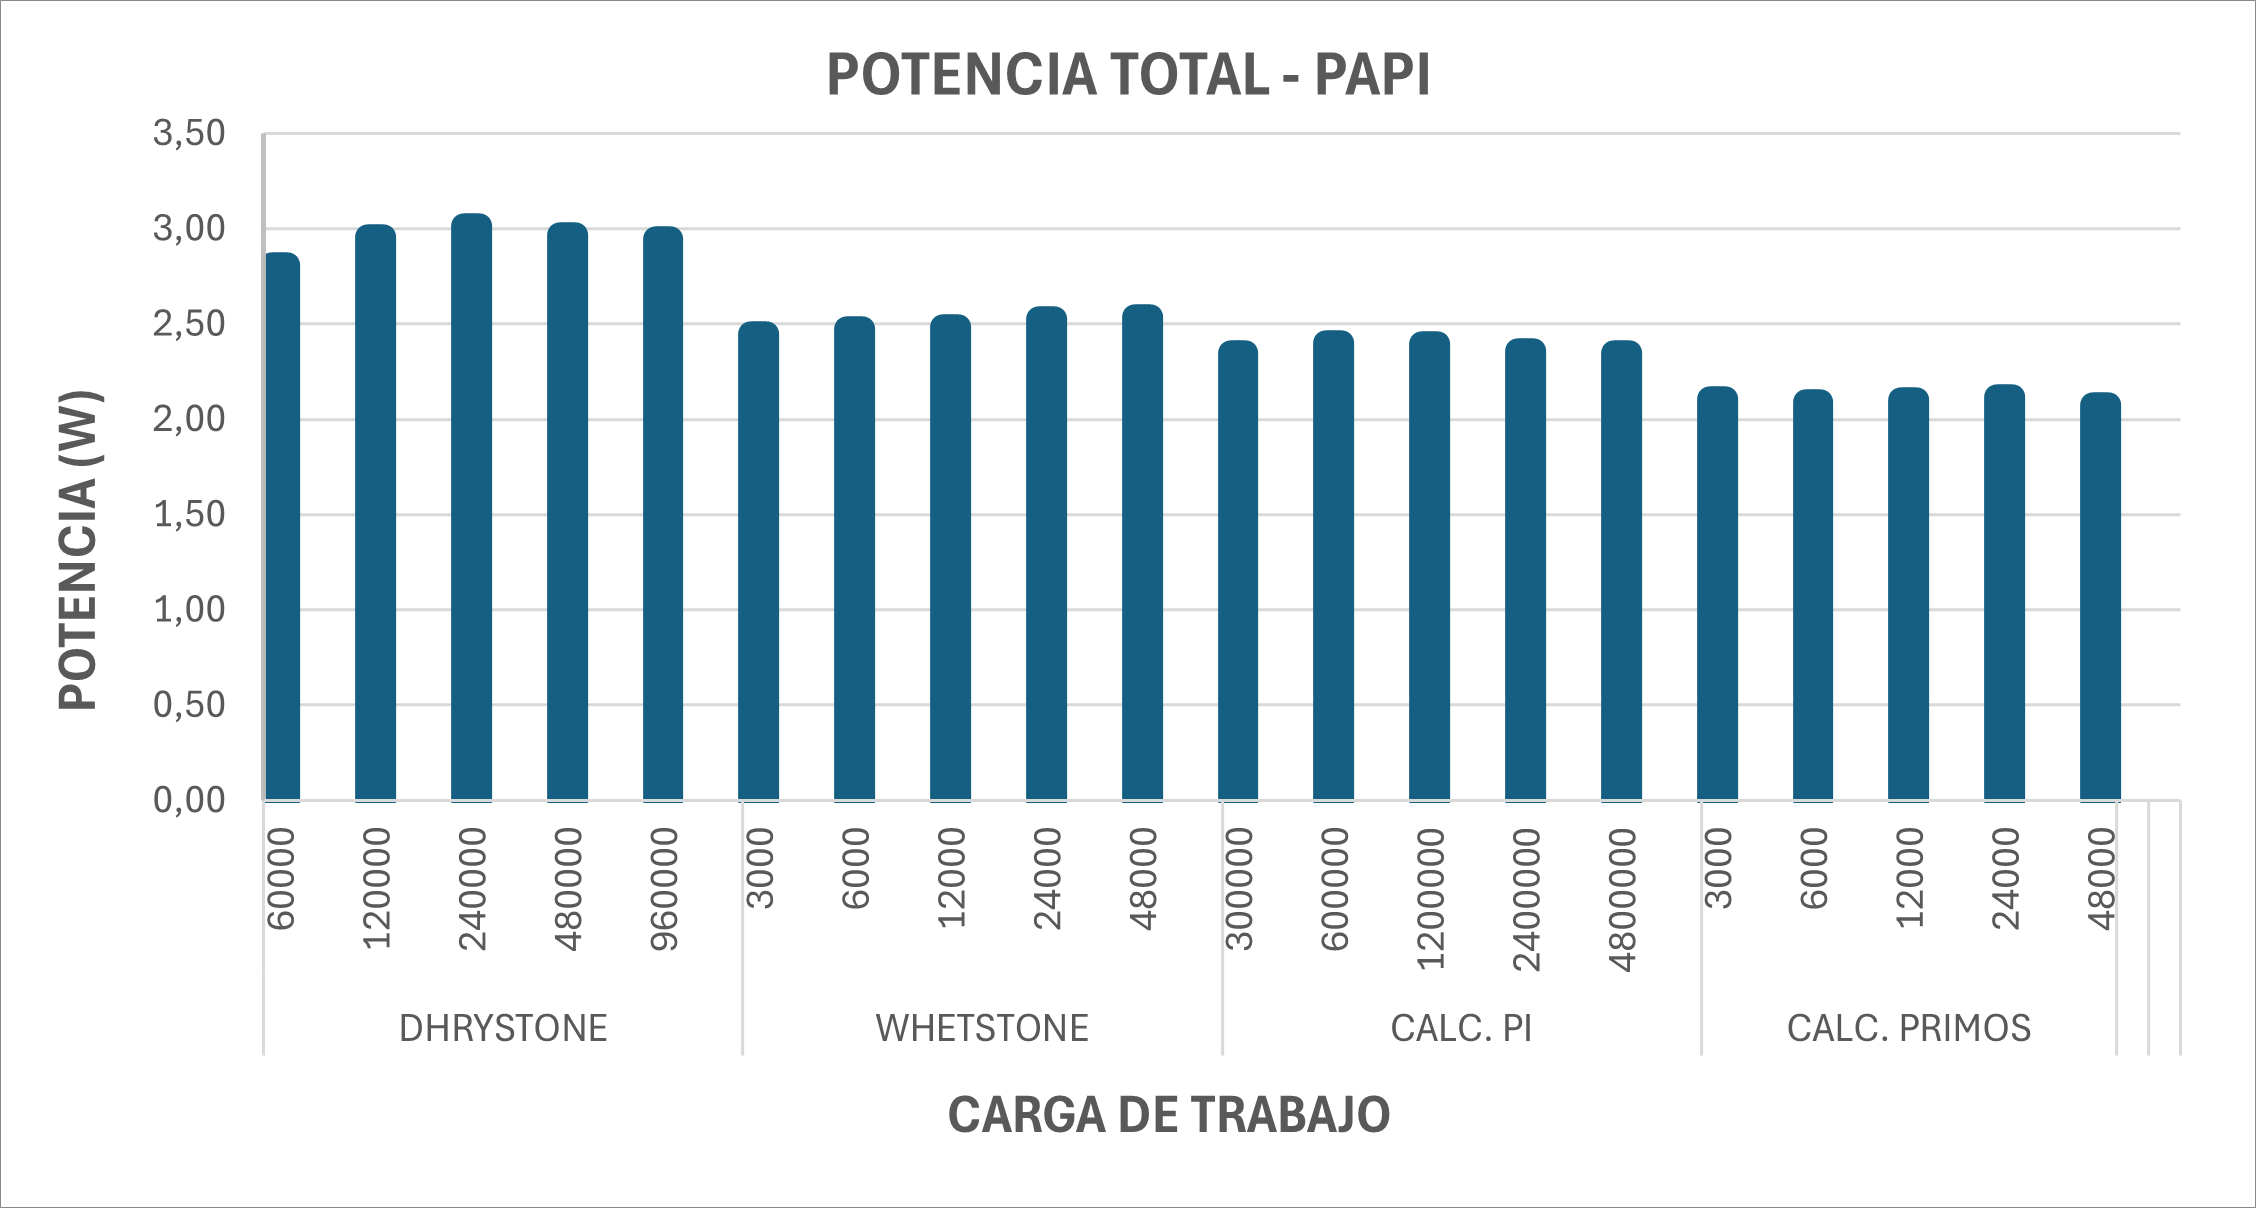
\includegraphics{figs/potenciaPAPI.png}}
    \caption{Potencia total de los \textit{benchmark} en PAPI}
    \label{fig:potenciaPAPI}
\end{figure}

Como como puede observarse en las figuras \ref{fig:potenciaGem5}, los valores de potencia son estables para cada carga de trabajo dentro de los \textit{benchmarks}, mientras que estos valores difieren entre los distintos tipos de \textit{benchmark}. Esto es debido a que en Gem5, las métricas obtenidas tras ejecutar el Cálculo de decimales de Pi, ha tenido los valores más bajos, haciendo que el valor de potencia total sea, por tanto, menor al resto. En \ref{fig:potenciaPAPI}, los valores de potencia son estables en todas las ejecuciones realizadas: en PAPI, las métricas para el cálculo de la potencia se han obtenido ejecutando las pruebas sobre la plataforma física, mediante registros \textit{hardware} de gran precisión y estabilidad, algo que en Gem5 es delegado a las estadísticas generadas por el propio \textit{software} de simulación.

Para poder realizar una comparativa de resultados entre ambos entornos, se muestran en la figura \ref{fig:diferenciaPotenciaGem5PAPI} las diferencias relativas a Gem5 sobre PAPI.

\begin{figure}[H]
    \centering
    \resizebox{0.8\linewidth}{0.3\textwidth}{
    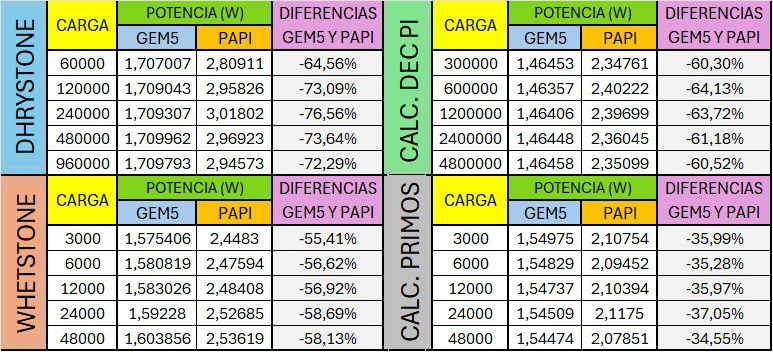
\includegraphics{figs/diferenciaPotenciaGem5PAPI.jpg}}
    \caption{Comparativa entre resultados de potencia obtenidos de Gem5 y PAPI}
    \label{fig:diferenciaPotenciaGem5PAPI}
\end{figure}

Con la figura anterior, se han sacado una serie de conclusiones:

\begin{enumerate}%[noitemsep]
    \item \textbf{Existe una diferencia considerable en los valores de potencia total entre Gem5 y PAPI}: esto es debido principalmente a la gran diferencia existente entre las métricas de Gem5 y sus equivalentes en PAPI, pues en Gem5 estos valores son considerablemente menores. Tal y como está expuesto en \ref{eq:modeloPotenciaDinamica}, a la hora de calcular la potencia dinámica total se tiene en cuenta cada uno de los modelos de potencia dinámica, los cuales poseen métricas concretas. Esto desemboca en que los valores obtenido con Gem5 sean un 76.56\% más bajo en el peor escenario de Dhrystone, un 58.69\% menor en el peor caso de Whetstone, un 64.13\% menor en el peor escenario al calcular decimales de Pi, y un 37.05\% más bajo al calcular números primos en el peor caso.

    \item \textbf{PAPI presenta unos valores superiores de potencia en todas los ejecuciones}: para todos los \textit{benchmarks} y respectivas cargas de trabajo, se obtienen con PAPI unos valores de potencia un 56.73\% superiores de media, aun habiéndose utilizado las mismas fórmulas: esto es debido a que las métricas obtenidas por \textit{software} con Gem5 no son igual de precisas que las aportadas por los registros contadores de bajo nivel, además de la problemática de haber modelado exclusivamente un subconjunto de componentes y conexiones de la plataforma en el simulador, y posibles imprecisiones resultantes a la hora del modelado de los mismos en Gem5.
\end{enumerate}

\section{Iteración 7 - Comparativa de resultados frente a mediciones con DMM}

En esta iteración se procederá a obtener las métricas de intensidad, durante las ejecuciones de cada uno de los \textit{benchmarks}, medida sobre el cable de alimentación de la plataforma Raspberry Pi 4. 

Para este propósito, se ha empleado un \ac{DMM}, que permitirá obtener mediciones de corriente precisas. Un DMM es un dispositivo que permite medir, sobre un \ac{IC} o cable, diversas magnitudes eléctricas como voltaje (tanto en corriente continua como alterna), corriente y resistencia. \cite{funcionamiento-dmm}.El funcionamiento consiste en la captación de las señales eléctricas analógicas provenientes del circuito o cable, mediante el uso de unas puntas, elemento conductor de electricidad conectado al DMM y al circuito o cable el cual se pretende realizar las mediciones. Estas medidas se convierten a valores digitales, los cuales se muestran en una pantalla, proporcionando lecturas precisas en las unidades disponibles (voltios, amperios, ohmios, etc.). En el contexto de este trabajo, las mediciones realizadas han sido de amperios exclusivamente.

\subsection{Lectura de especificaciones del \ac{DMM}}

Primeramente, se ha realizado una lectura de la documentación del \ac{DMM} utilizado para verificar la caracterización a nivel energético del prototipo. En un principio, este aparato era el OWON XDM-2041~\cite{documentacionDMM}, sin embargo, durante las pruebas, se comprobó que los tiempos de ejecución no eran acordes a lo previsto, por lo que se decidió utilizar otro \ac{DMM}.

El DMM utilizado finalmente es Velleman DVM1200 \cite{documentacionDMM-alt}, mostrado en la figura ~\ref{fig:DMM}. Además, puede verse un resumen de las características más importantes de este dispositivo en la tabla ~\ref{tab:caracteristicasDMM}. Con este dispositivo, se pudieron obtener mejores resultados que con el primero. Aunque se desconoce la causa del problema, se sospecha que las resistencias internas del primer \ac{DMM} son muy altas, lo que provoca bajadas de voltaje en el dispositivo, ralentizando en gran medida el sistema y aportando resultados erróneos.

\begin{figure}[H]
    \centering
    \begin{minipage}[b]{.45\textwidth}
    \centering
        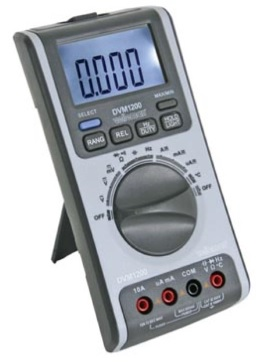
\includegraphics[width=0.4\textwidth, height=0.55\textwidth]{figs/dvm1200.jpg}
        \caption{\ac{DMM} utilizado. Fuente: \cite{dmm-alternativo}}
        \label{fig:DMM}
    \end{minipage}%
    \begin{minipage}[b]{.45\textwidth}
        \scriptsize
        \centering
        \resizebox{6.5cm}{!}{
        \begin{tabular}{|
        >{\columncolor[HTML]{C0C0C0}}c c|}
        \hline
        \multicolumn{2}{|c|}{\cellcolor[HTML]{C0C0C0}\textbf{Especificaciones del DMM utilizado}} \\ \hline
        \multicolumn{1}{|c|}{\cellcolor[HTML]{C0C0C0}\textbf{Modelo}} & \cellcolor[HTML]{FFFFFF}VELLEMAN DVM1200 \\ \hline
        \multicolumn{1}{|c|}{\cellcolor[HTML]{C0C0C0}\textbf{Counts}} & \cellcolor[HTML]{FFFFFF}55000 \\ \hline
        \multicolumn{1}{|c|}{\cellcolor[HTML]{C0C0C0}\textbf{Mediciones de voltaje}} & Desde 0.6V hasta 1000V \\ \hline
        \multicolumn{1}{|c|}{\cellcolor[HTML]{C0C0C0}\textbf{Mediciones de corriente}} & \cellcolor[HTML]{FFFFFF}Desde 600uA hasta 10A \\ \hline
        \multicolumn{1}{|c|}{\cellcolor[HTML]{C0C0C0}\textbf{Muestreo}} & \cellcolor[HTML]{FFFFFF}250ms (no configurable) \\ \hline
        \multicolumn{1}{|c|}{\cellcolor[HTML]{C0C0C0}\textbf{Número de muestras}} & Sin límite \\ \hline
        \multicolumn{1}{|c|}{\cellcolor[HTML]{C0C0C0}\textbf{Comunicación}} & Puerto serie (USB) \\ \hline
        \end{tabular}}
        \caption{Especificaciones DMM}
        \label{tab:caracteristicasDMM}
    \end{minipage}
\end{figure}

Tal y como se muestra en las especificaciones, el término \textit{counts} se refiere al número de divisiones o incrementos en la escala de lectura del \ac{DMM}. Es decir, 6000 \textit{counts} será capaz de medir desde 0000 a 5999, Al ser cuatro dígitos, la precisión decimal será de 3 dígitos, mientras que el otro dígito, que van de 0 a 6, serán para medir el valor entero de la lectura. En este contexto, los valores se refieren a \emph{CC} (Corriente Continua) y siempre dependiendo del rango de medición seleccionado.

\subsection{Preparación del entorno de pruebas}
\label{subs:diseño}

Una vez seleccionado el \ac{DMM}, se ha realizado el diseño y montaje del circuito para la medición de la intensidad sobre el cable de alimentación de la plataforma. Este cable se ha modificado para poder conectar las puntas del multímetro al mismo. El resultado se puede ver en la figura ~\ref{fig:montaje}. Respecto al montaje real del circuito para las mediciones, en la figura ~\ref{fig:intensidad} se muestra el entorno de medición. Como puede apreciarse, solamente se ha realizado prueba de intensidad: esto es debido a que se ha considerado al voltaje como \emph{constante} (5 Voltios). Esto ha permitido agilizar las pruebas realizadas, ya que el \ac{DMM} utilizado no es capaz de medir corriente y voltaje al mismo tiempo.

% \begin{figure}[h]
%     \centering
%     \resizebox{0.45\linewidth}{0.3\textwidth}{
%     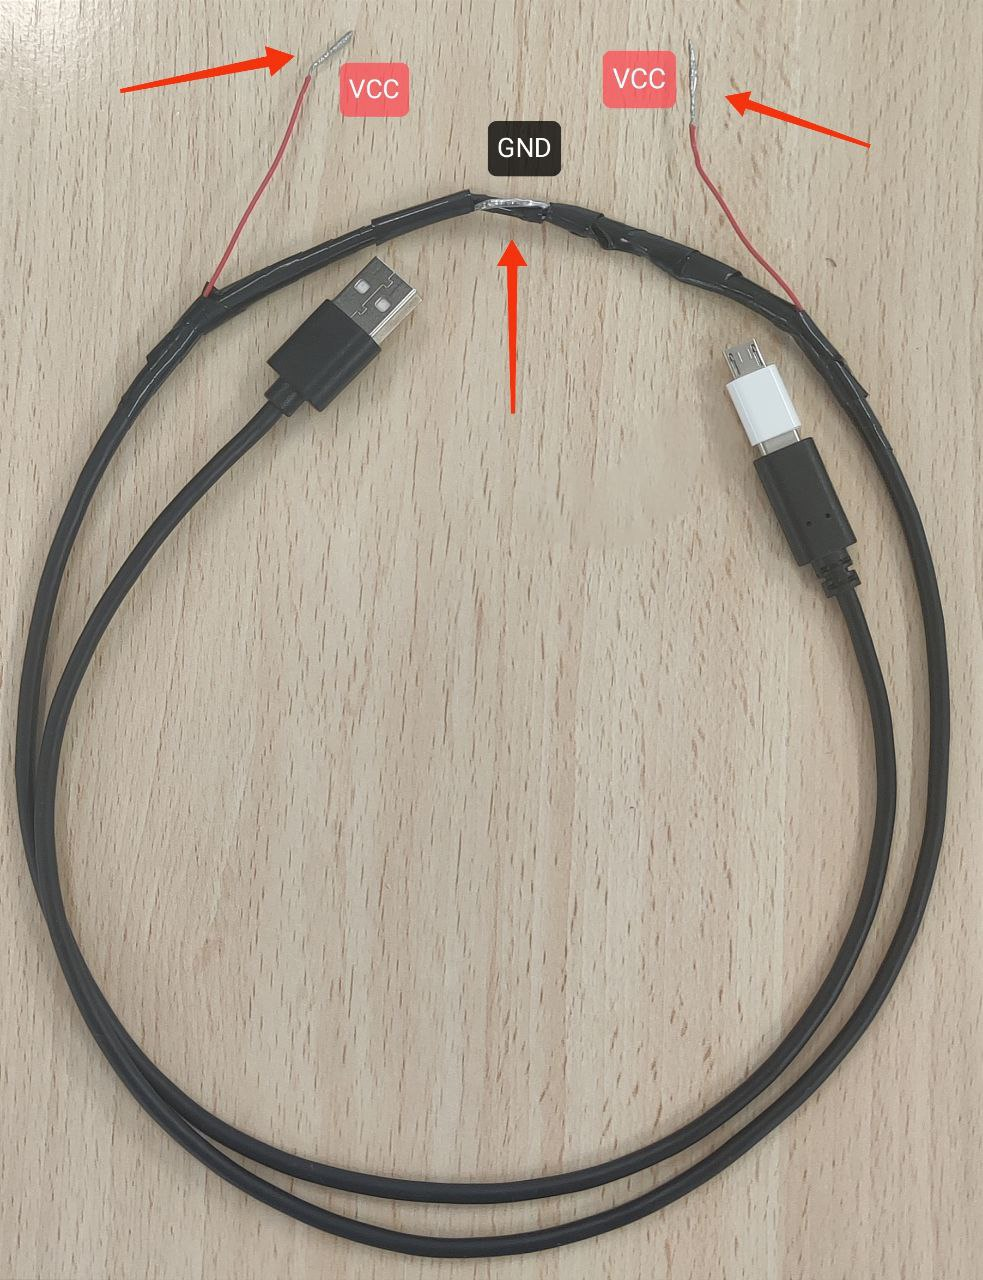
\includegraphics{figs/cable.jpg}} % cambiar por montaje.jpeg
%     \caption{Montaje para las pruebas de corriente reales}
%     \label{fig:montaje}
% \end{figure}

% \begin{figure}[h]
%     \centering
%     \resizebox{0.7\textwidth}{0.3\textwidth}{
%     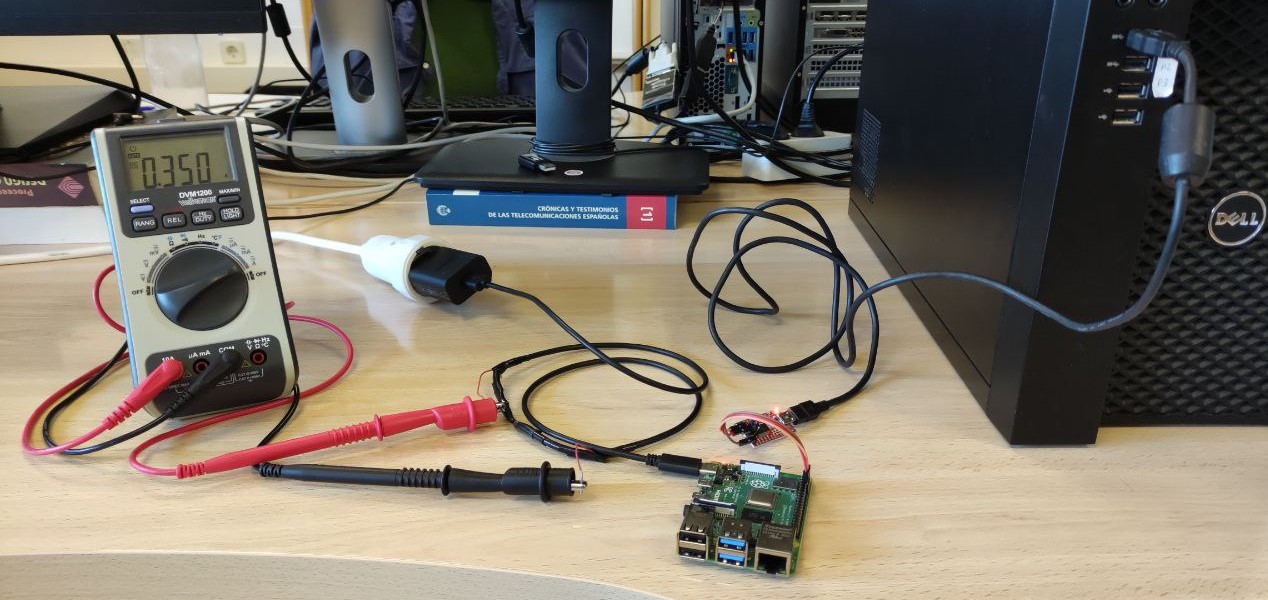
\includegraphics{figs/dmm_intensidad.jpg}}
%     \caption{Medición de corriente sobre el modelo de pruebas}
%     \label{fig:intensidad}
% \end{figure}

\begin{figure}[H]
    \centering
    \begin{minipage}{0.29\textwidth}
    \centering
        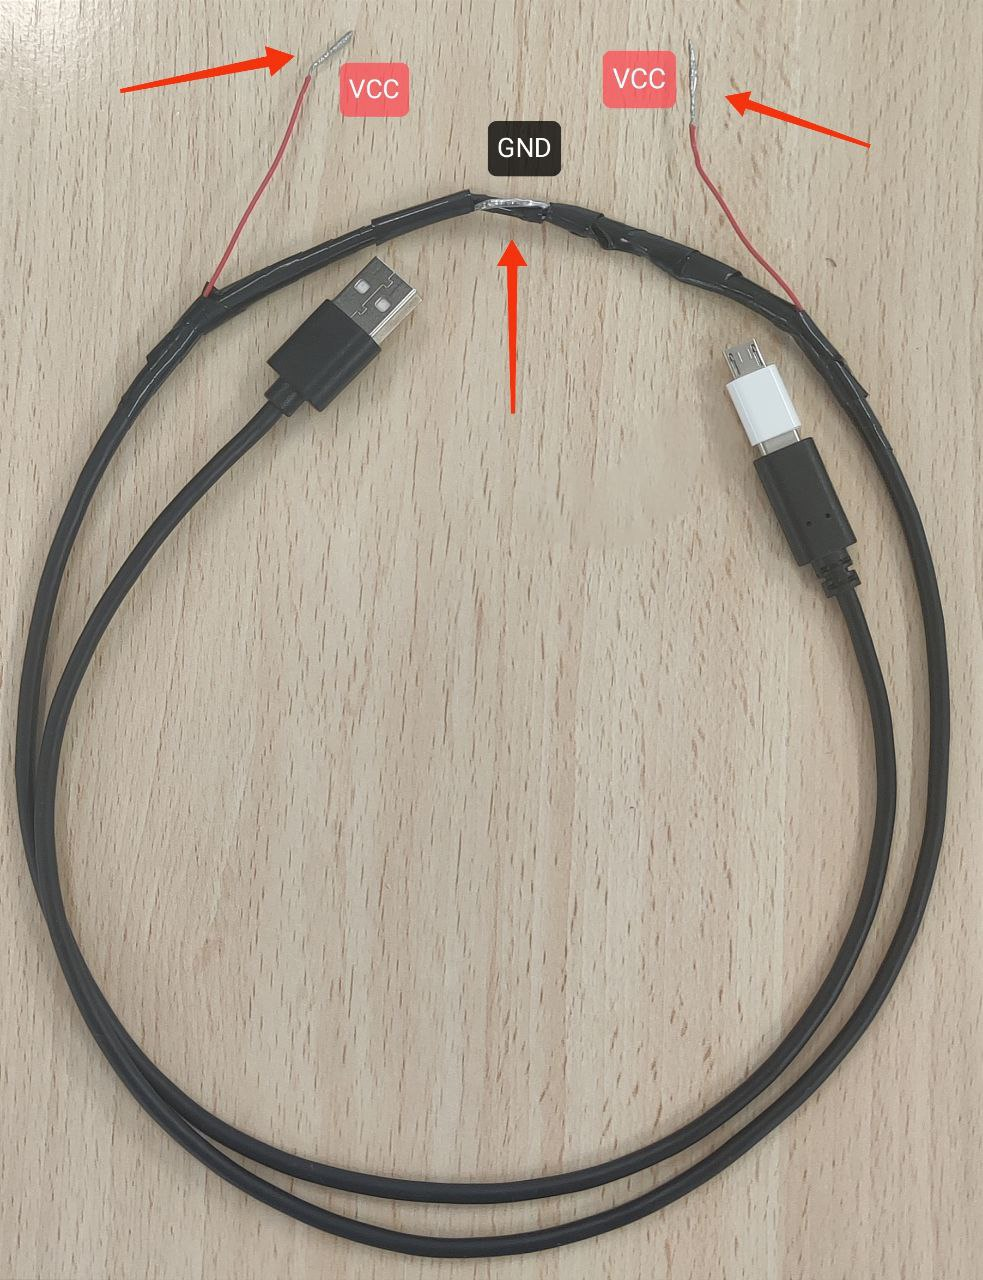
\includegraphics[width=\textwidth, height=5cm]{figs/cable.jpg}
        \caption{Cable utilizado}
        \label{fig:montaje}
    \end{minipage}%
    \vspace*{\fill}
    \begin{minipage}{.69\textwidth}
        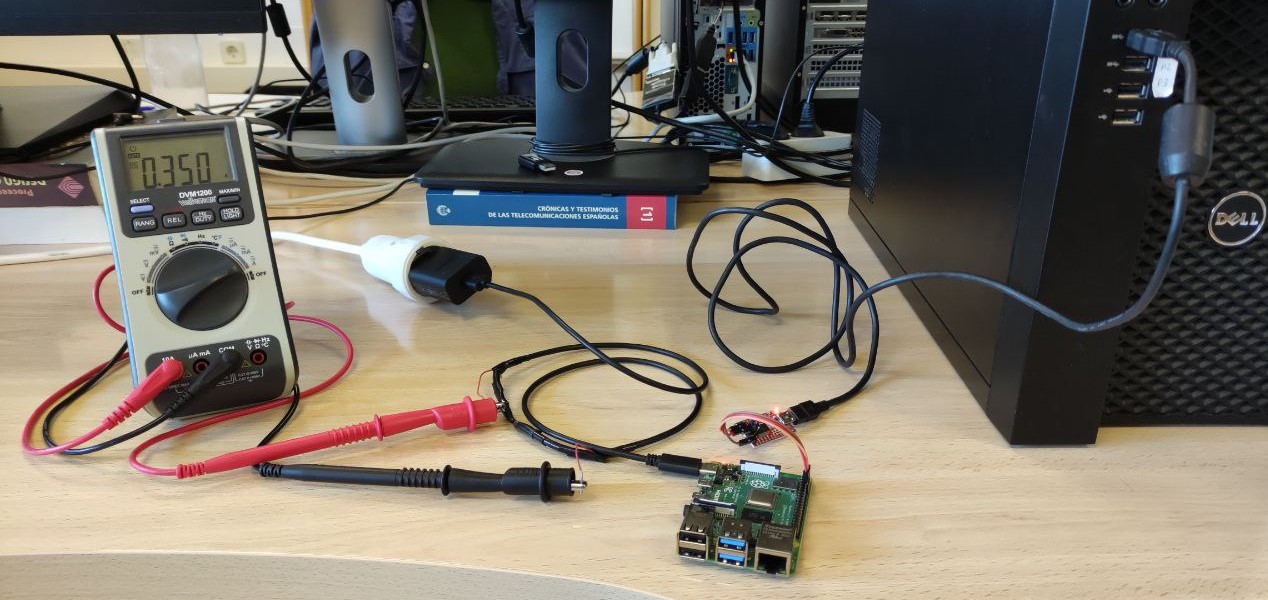
\includegraphics[width=\textwidth,height=5cm]{figs/dmm_intensidad.jpg}
        \caption{Medición de corriente sobre el cable de alimentación de la plataforma}
        \label{fig:intensidad}
    \end{minipage}
\end{figure}


Llegados a este punto, es posible preguntarse si no habría sido más preciso realizar las mediciones sobre los componentes, y no sobre un cable de corriente; debido a reguladores de voltaje, capacitores, y resistencias dinámicas/fijas \cite{schematics-rpi}, y de un desconocimiento general en microelectrónica, es demasiado complejo, en el contexto de este trabajo, realizar mediciones de esta forma. 

\subsection{Resultados y conclusiones}

Tras el montaje del circuito, se ha puesto a prueba con la ejecución de los \textit{benchmarks} en la plataforma de cómputo, tomándose las medidas de corriente con la función de \textit{datalogging} del \ac{DMM}, siendo los resultados mostrados la media aritmética de 4 ejecuciones del mismo.

Para poder obtener los datos por el puerto serie \ac{USB}, ha sido necesario el uso de un programa procedente de un repositorio de GitHub \cite{dmm-github-repo}, el cual decodifica las lecturas del puerto serie para poder obtener el resultado real. Debido al poco muestreo del \ac{DMM} (4 muestras por segundo) se ha asumido el valor más alto de corriente obtenido durante la ejecución de cada carga de trabajo para todos los \textit{benchmarks}. Los resultados máximos de corriente obtenidos por \textit{benchmark}d se presentan en la tabla \ref{fig:valoresCorrienteDMM}. 

\begin{table}[h]
\centering
    \begin{tabular}{|c|c|}
      \hline
      \rowcolor[HTML]{C0C0C0}
      \multicolumn{2}{|c|}{\cellcolor[HTML]{C0C0C0} \textbf{VALORES DMM}} \\ \hline
      \rowcolor[HTML]{EFEFEF}
      \multicolumn{1}{|c|}{\cellcolor[HTML]{EFEFEF} \textbf{BENCHMARK}} &  \textbf{CORRIENTE (A)} \\ \hline
      \multicolumn{1}{|c|}{ Dhrystone} &  0.517 \\ \hline
      \multicolumn{1}{|c|}{ Whetstone} &  0.502 \\ \hline
      \multicolumn{1}{|c|}{ Cálculo decimales Pi} &  0.508 \\ \hline
      \multicolumn{1}{|c|}{ Cálculo de primos} &  0.481 \\ \hline
    \end{tabular}
\caption{Valores de corriente máximos obtenidos con el DMM utilizado}
\label{fig:valoresCorrienteDMM}
\end{table}

Finalmente, tras obtener los valores de corriente, se ha calculado la potencia total con la fórmula expuesta en \ref{eq:potencia2}. En la figura \ref{fig:potenciaDMM} se muestra en forma de gráfica los resultados de potencia global obtenidos mediante el DMM.  Estos valores serán utilizados en la fórmula de la energía mostrada en \ref{eq:energia} para Gem5, PAPI, y el DMM, y así validar el modelo propuesto en este trabajo.

\begin{figure}[H]
    \centering
    \resizebox{0.85\linewidth}{0.4\textwidth}{
    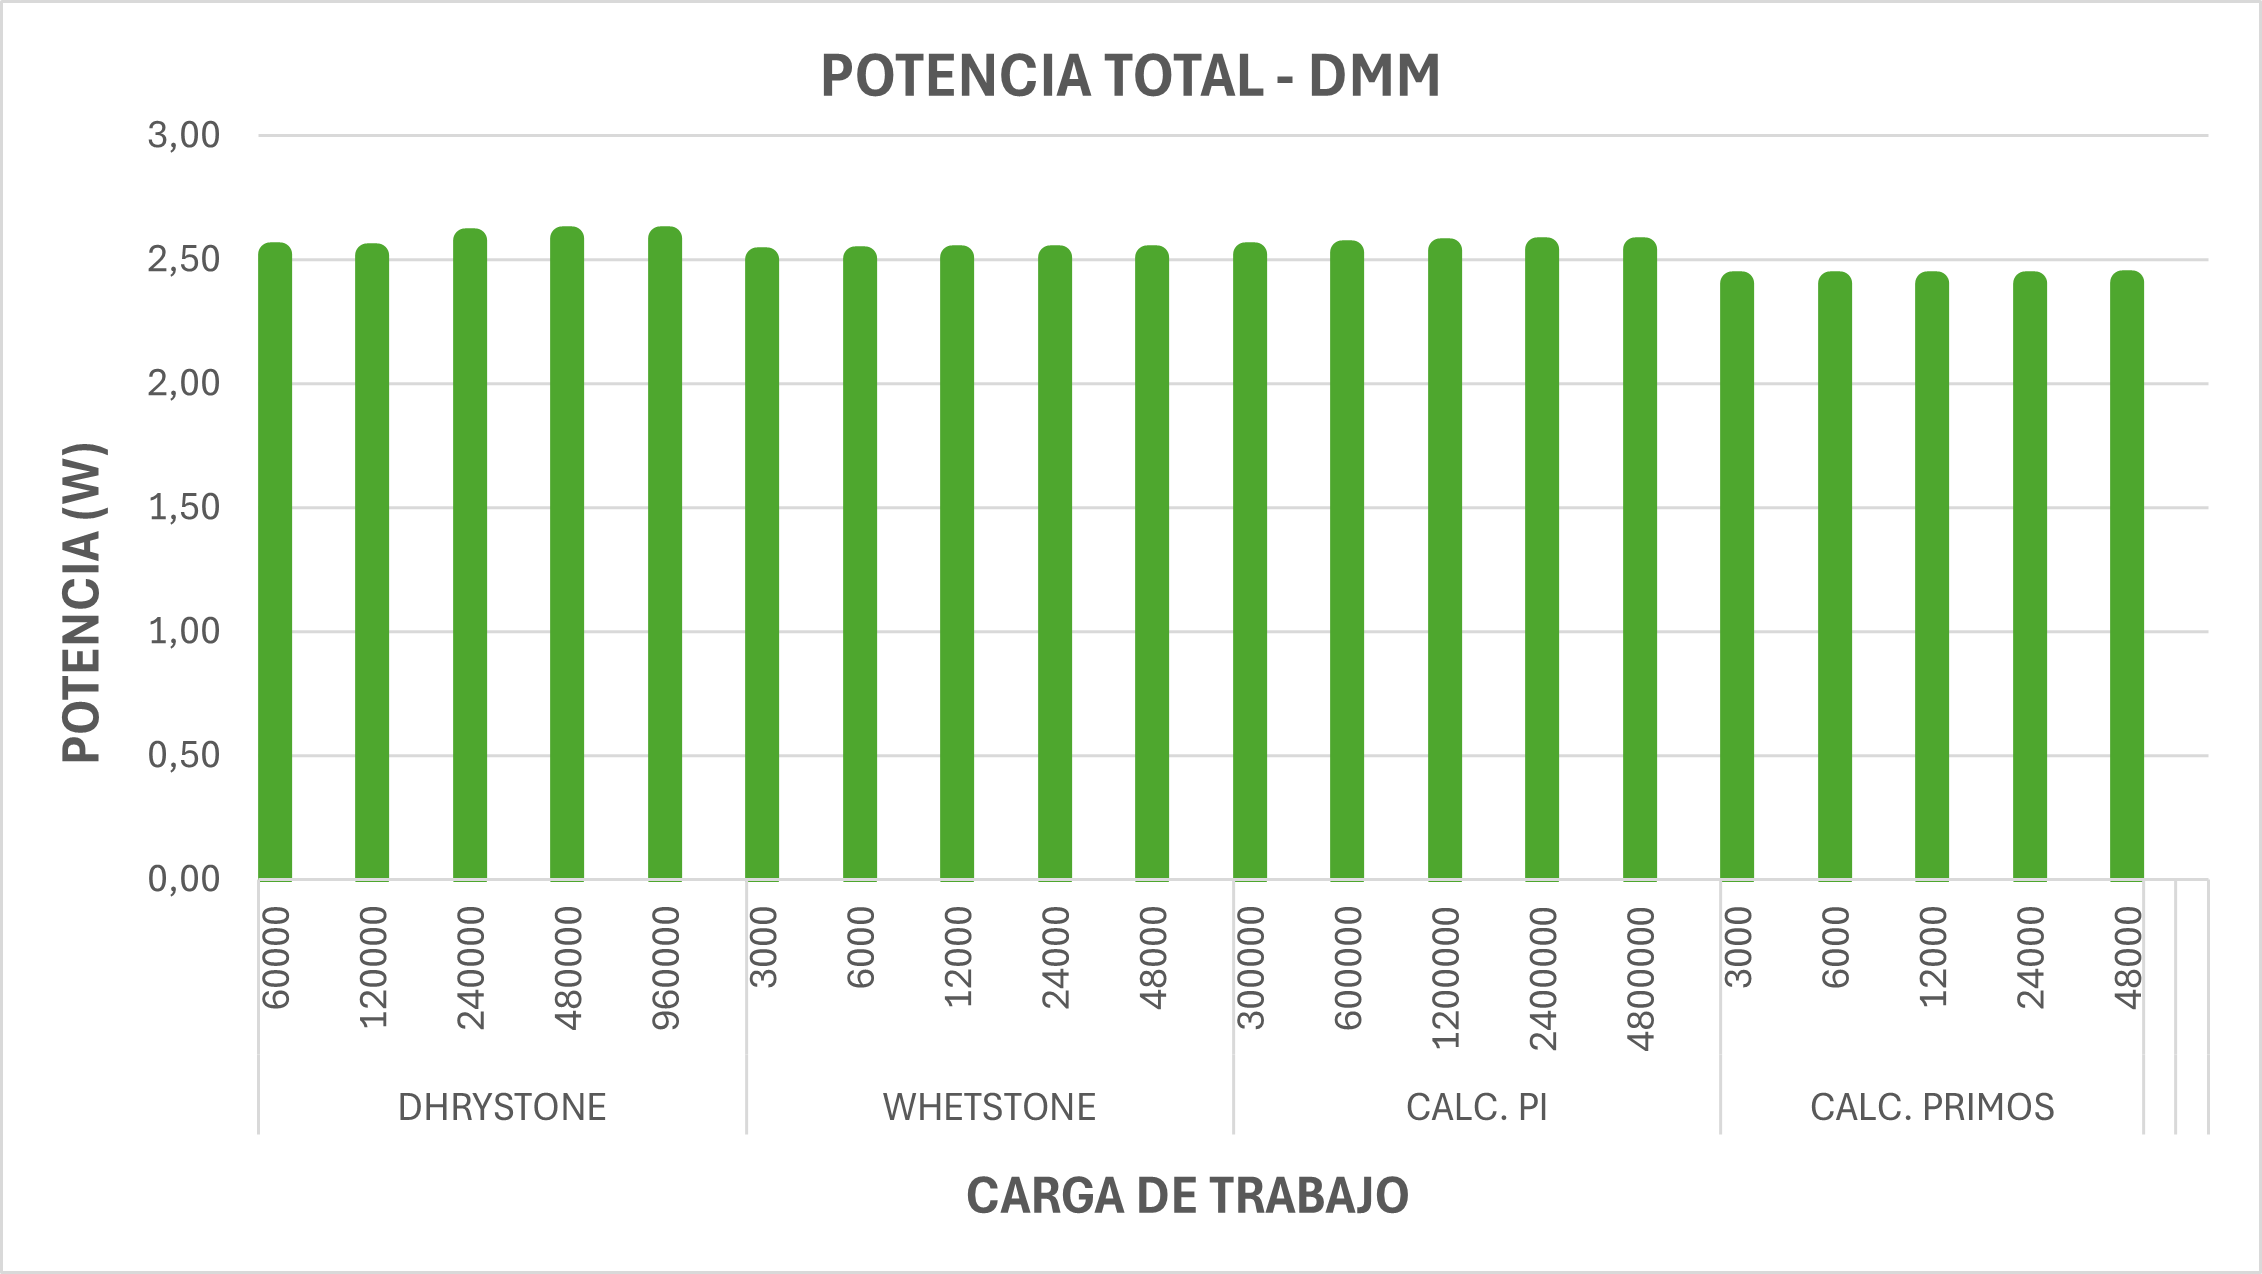
\includegraphics{figs/potenciaDMM.png}}
    \caption{Potencia global de los \textit{benchmark} en DMM}
    \label{fig:potenciaDMM}
\end{figure}

Como puede observarse en \ref{fig:potenciaDMM}, los valores de potencia obtenidos en todas las ejecuciones son prácticamente idénticos entre sí; en las ejecuciones realizadas con el DMM, se ha calculado la potencia mediante la intensidad máxima alcanzada en cada carga de cada \textit{benchmark}, medida con el DMM, mientras que se ha asumido, para este trabajo, un voltaje \emph{constante} en todas las pruebas realizadas. Para realizar una comparativa entre los valores obtenidos con el DMM y los valores obtenidos con Gem5 y PAPI, se muestra en la figura \ref{fig:diferenciaPotenciaDMM} las diferencias del primero frente a los otros dos escenarios.

\begin{figure}[H]
    \centering
    \resizebox{1\linewidth}{0.32\textwidth}{
    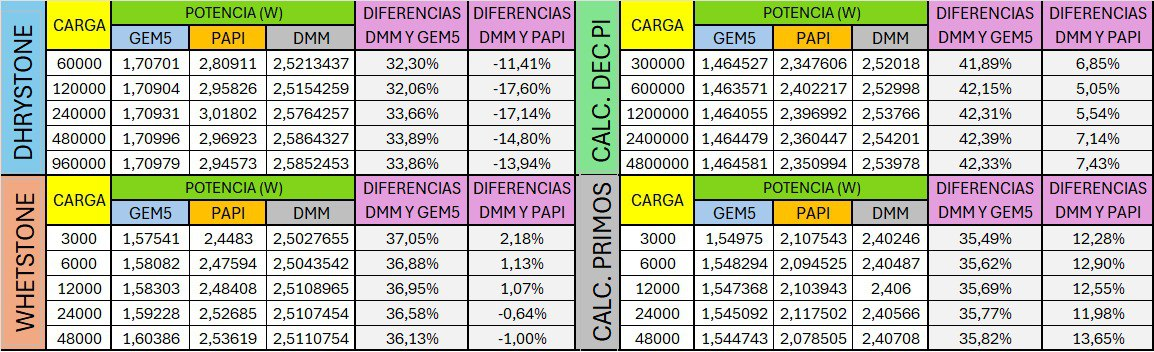
\includegraphics{figs/diferenciaPotenciaDMM.jpg}}
    \caption{Comparativa entre resultados de potencia obtenidos de DMM, Gem5 y PAPI}
    \label{fig:diferenciaPotenciaDMM}
\end{figure}

Las conclusiones fruto de dicha figura son las siguientes:

\begin{enumerate}%[noitemsep]
    \item \textbf{Los valores de potencia obtenidos con el DMM son similares a los recogidos con PAPI}: como puede observarse en la gráfica de potencia de PAPI en \ref{fig:potenciaPAPI} y en la presentada arriba, los resultados de potencia calculados son muy parecidos entre sí, para cada carga de trabajo de cada \textit{benchmark}, obteniendo en DMM hasta un 17\% más en Dhrystone, un 2\% menos en Whetstone, un 7\% en el cálculo de decimales de Pi, y un 13\% al calcular números primos. Este parecido en resultados se debe a que, a la hora de medir la corriente del cable de alimentación con el DMM, como a la hora de aplicar la fórmula de potencia total en PAPI, ambos se han ejecutado sobre la plataforma física, obteniendo, por un lado, unos valores de corriente fiables gracias al DMM, y por otro, unas métricas precisas gracias al uso de contadores \textit{hardware}, haciendo que ambos escenarios, PAPI y DMM posean unos valores de potencia similares entre sí. 
    \item \textbf{Los valores de potencia del DMM difieren considerablemente con los de Gem5}: debido a la diferencia comentada previamente entre los valores de potencia de Gem5 y PAPI, sucede, por tanto, la misma problemática al comparar Gem5 y DMM, siendo los valores del segundo superiores en más de un 32\% en todos las cargas de trabajo de Dhrystone, subiendo a un 36\% más en todas las de Whetstone, alcanzando más de un 41\% en todas las cargas de trabajo del \textit{benchmark} del cálculo de decimales del número Pi, y un 35\% más en todas las ejecuciones realizadas al calcular números primos. Nuevamente, las razones de estas diferencias radican en las métricas obtenidas con el simulador, a falta de modelado de más componentes dentro de la plataforma simulada, y a imprecisiones en el modelado del procesador y de las cachés.
\end{enumerate}

\section{Iteración 8 - Validación del marco teórico de medición}

Una vez realizada la ejecución de los programas de \textit{benchmark} ya presentados, se realizará la comparación entre los valores recogidos con las herramientas \ac{PAPI} y Gem5 frente a las mediciones obtenidas con el DMM, sobre el cable de alimentación físico de la plataforma seleccionada. Posteriormente, se dará una serie de conclusiones relativas a los resultados obtenidos.

\subsection{Resultados y conclusiones}

Se ha generado un gráfica de la energía consumida, que unifica a la vez los escenarios de Gem5, PAPI, y DMM, mostrando el consumo energético global obtenido en cada uno, permitiendo visualizar similitudes y diferencias entre ellos. En la figura \ref{fig:comparacionEnergia} se muestra la energía consumida para distintos benchmarks y cargas de trabajo en Gem5, PAPI y DMM. A continuación, se presentan las principales conclusiones derivadas de esta comparación.

\begin{figure}[H]
    \centering
    \resizebox{0.9\linewidth}{0.85\textwidth}{
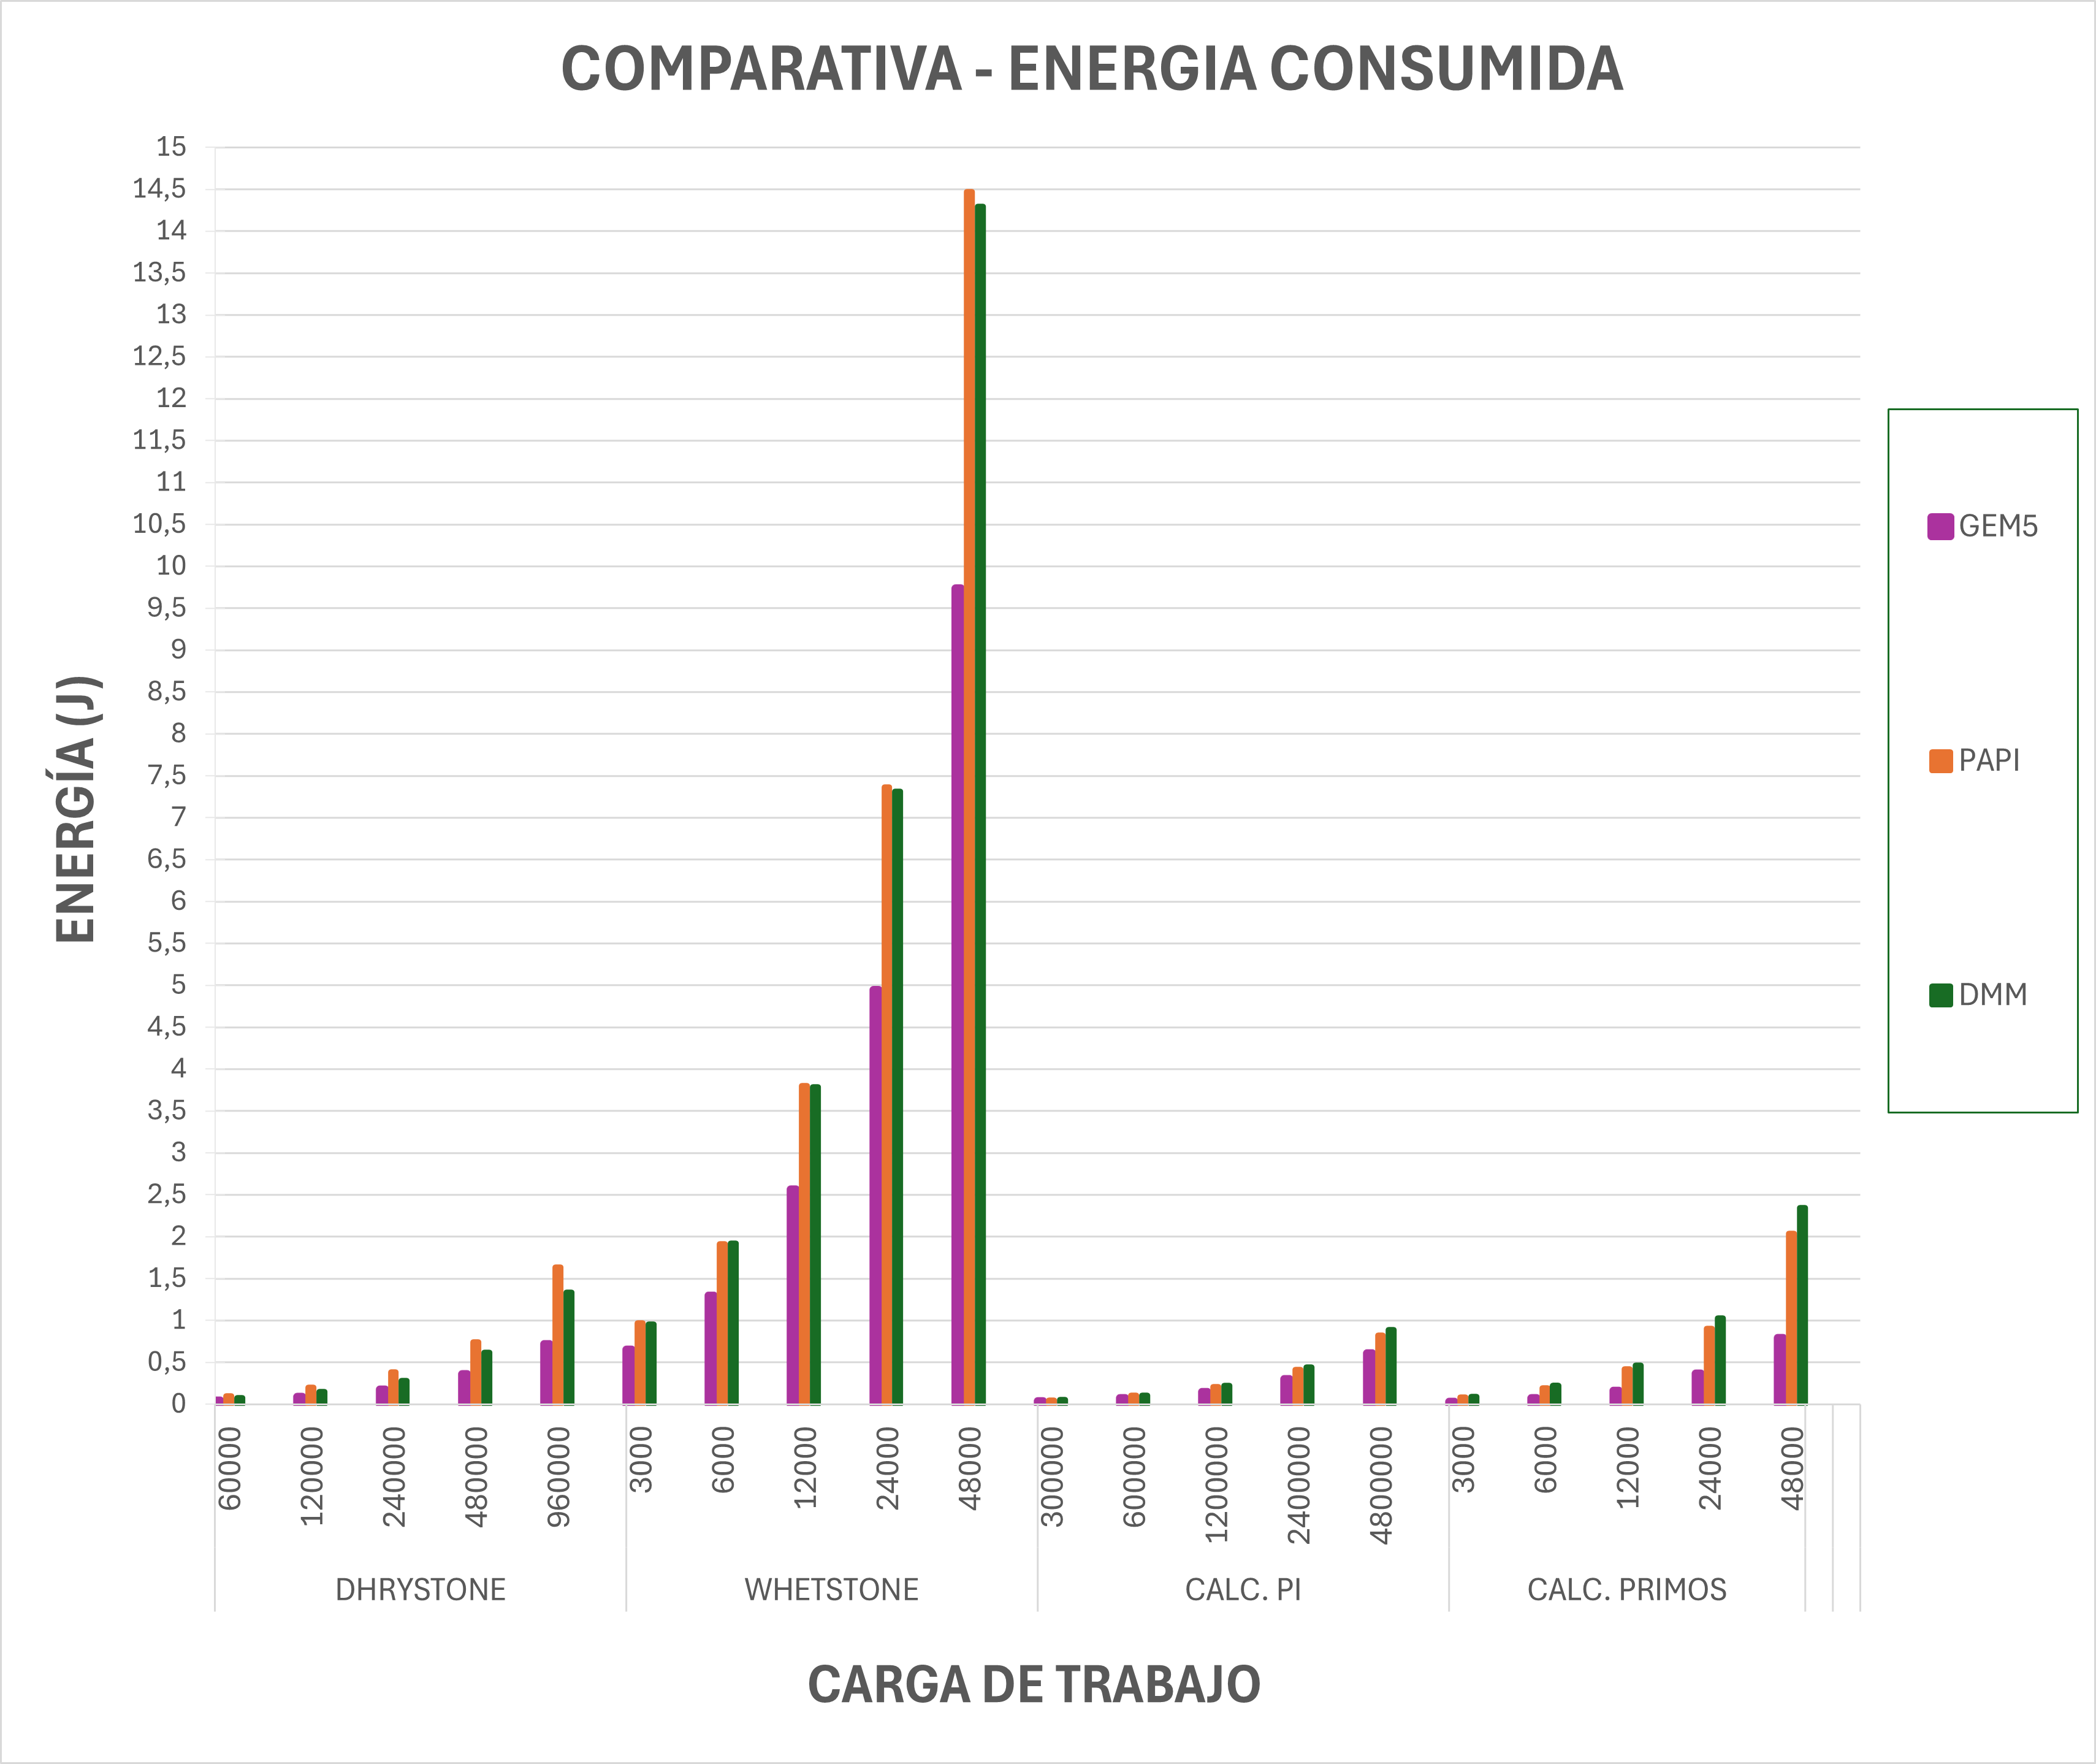
\includegraphics{figs/comparacionEnergia.png}}
    \caption{Energía consumida por los \textit{benchmarks} en Gem5, PAPI y DMM}
    \label{fig:comparacionEnergia}
\end{figure}

Como puede observarse en la figura \ref{fig:comparacionEnergia}, conforme aumenta la carga de trabajo de cada uno de los \textit{benchmarks}, aumenta la energía consumida, de forma que la energía es dependiente de los tiempos de ejecución, en todos los escenarios. También hay que destacar las grandes diferencias del \textit{benchmark} Whetstone frente al resto: esto es debido a que Whetstone es el \textit{benchmark} que más tiempo de ejecución requiere, impactando, por tanto, en la energía consumida. Las razones a los altos tiempos de ejecución son debido la sensibilidad del propio código del programa a optimizaciones \cite{referencia-tiempos-whetstone},ya que las operaciones de punto flotante se realizan sobre arrays 1x1 y no directamente sobre las datos, lo que desemboca en un uso intensivo de las cachés y la necesidad de buscar los datos, aumentando el tiempo total. En la actualidad, los compiladores modernos optimizan estas tareas fácilmente; sin embargo, en este trabajo, todas las compilaciones se han realizado sin optimización alguna. 

Además, puede apreciarse en \ref{fig:comparacionEnergia} una similitud entre las mediciones de PAPI y las del DMM, diferenciándose en un mayor grado en la ejecución de la carga de 960000 instrucciones Dhrystone, así como en el cálculo de 48000 números primos. Esto sucede porque el modelo de energía teórico planteado resulta ser más preciso en aquellos \textit{benchmarks} enfocados en utilizar las unidades de punto flotante; como puede apreciarse en dicha gráfica, Whetstone y el Cálculo de decimales de Pi presentan unas mediciones más parecidas. La conclusión de esto es que la plataforma real es capaz de reducir al máximo el consumo de aquellas unidades funcionales y periféricos que no se utilizan: el objetivo en las pruebas es realizar operaciones intensivas en cómputo, saturando el procesador, estando los modelos de potencia dinámica enfocados en las diferentes unidades funcionales de éste, de ahí el gran parecido entre ambos escenarios. A pesar de todo, resulta interesante cómo los valores de consumo son parecidos, aún siendo en escenarios totalmente distintos, destacándose:

\begin{itemize}
    \item El voltaje que se maneja sobre el cable \ac{USB} es superior al utilizado por el propio procesador, siendo el voltaje de 5 Voltios para las pruebas con el DMM, y 0.8688 Voltios el valor de voltaje utilizado para las ejecuciones sobre PAPI. 
    
    \item El cable utilizado para las pruebas con el DMM alimenta a toda la plataforma de cómputo, incluyendo, además del procesador, periféricos y otros componentes secundarios \cite{schematics-rpi}, mientras que, en los modelos de potencia dinámica, aplicados sobre las ejecuciones realizadas con PAPI solamente se tiene en cuenta el componente procesador.
\end{itemize}

\subsection{Validación frente a las mediciones con el DMM}

Para finalizar, se presentan en \ref{gem5-vs-dmm} y \ref{papi-vs-dmm} las conclusiones fruto de los resultados de energía obtenidos para Gem5 y PAPI, así como la decisión adoptada sobre la validación de ambos.

\subsubsection{Validación del modelo teórico en Gem5}
\label{gem5-vs-dmm}

Sobre la decisión tomada sobre la correcta o incorrecta validación del modelo de energía propuesto sobre las simulaciones con Gem5, se ha determinado que el modelo teórico realizado en Gem5 \textbf{no es válido}, debido a lo siguiente:

\begin{enumerate}%[noitemsep]
    \item \textbf{Los tiempos de ejecución en Gem5 son muy dispares}: tal y como se explicó en \ref{conc:tiemposGem5PAPI}, debido a la incapacidad de modelar correctamente las latencias en las simulaciones ejecutadas, el tiempo de ejecución en Gem5 es menor frente a las ejecuciones con el DMM, desembocando en valores de energía más reducidos que los dados por la plataforma real. 
    \item \textbf{No se ha modelado toda la plataforma en Gem5}: debido a la complejidad para construir de forma precisa una plataforma real al completo en cualquier tipo de simulador, es difícil obtener unos resultados que sean lo más parecidos posibles a la realidad. En el contexto de este trabajo, se ha modelado el componente procesador, destacando sus unidades de cálculo y cachés, aunque con limitaciones por falta de información relativa a características sobre políticas de reemplazo y tecnologías en los buses de interconexión, entre otros. Por ejemplo, a la hora de calcular un número mediante las \ac{ALU} o \ac{FPU}, no se tenga las precisiones temporales (latencias) acordes a la plataforma real. Estas problemáticas hacen imposible, en los plazos de entrega del proyecto, modelar un comportamiento idéntico al real. 
\end{enumerate}

\subsubsection{Validación del modelo teórico en PAPI}
\label{papi-vs-dmm}

Sobre la decisión tomada sobre la correcta o incorrecta validación del modelo de energía propuesto sobre las simulaciones con Gem5, se ha determinado que el modelo teórico realizado en Gem5 \textbf{es válido}, debido a las siguientes conclusiones:

\begin{enumerate}%[noitemsep]
    \item \textbf{El modelo teórico de energía en PAPI es capaz de obtener unos valores de consumo parecidos a la realidad}: esto es gracias a la adición de los conceptos de potencia estática y dinámica, así como la capacitancia y el factor de actividad. En el trabajo previo \cite{antoniomateo}, se consideró a los componentes identificados como los más representativos a nivel energético, en un permamente estado \emph{activo}, siendo éste el estado más pesimista posible en términos de consumo. Sin embargo, durante el tiempo de ejecución de un programa, todo componente pasa por diversos estados, por ejemplo, \textit{idle}, bajando su consumo energético cuando no está siendo utilizado intensivamente. 
    
    \item \textbf{El uso de contadores para los eventos hardware proporciona métricas precisas y fiables}: PAPI, al igual que el DMM, utiliza la plataforma física para realizar las pruebas, de forma que las métricas necesarias para conformar el modelo teórico se obtienen mediante la lectura de contadores \textit{hardware} de gran precisión, obteniendo unos valores de potencia más parecidos que con Gem5. Además, al utilizar ambos la plataforma física, los tiempos de ejecución serán también muy similares, por lo que la energía consumida, cuya fórmula puede verse en \ref{eq:energiaModelo2}, se tendrá un gran parecido entre ambos.
\end{enumerate}

\clearpage